\documentclass[twoside]{book}

% Packages required by doxygen
\usepackage{calc}
\usepackage{doxygen}
\usepackage{graphicx}
\usepackage[utf8]{inputenc}
\usepackage{makeidx}
\usepackage{multicol}
\usepackage{multirow}
\usepackage{textcomp}
\usepackage[table]{xcolor}

% Font selection
\usepackage[T1]{fontenc}
\usepackage{mathptmx}
\usepackage[scaled=.90]{helvet}
\usepackage{courier}
\usepackage{amssymb}
\usepackage{sectsty}
\renewcommand{\familydefault}{\sfdefault}
\allsectionsfont{%
  \fontseries{bc}\selectfont%
  \color{darkgray}%
}
\renewcommand{\DoxyLabelFont}{%
  \fontseries{bc}\selectfont%
  \color{darkgray}%
}

% Page & text layout
\usepackage{geometry}
\geometry{%
  a4paper,%
  top=2.5cm,%
  bottom=2.5cm,%
  left=2.5cm,%
  right=2.5cm%
}
\tolerance=750
\hfuzz=15pt
\hbadness=750
\setlength{\emergencystretch}{15pt}
\setlength{\parindent}{0cm}
\setlength{\parskip}{0.2cm}
\makeatletter
\renewcommand{\paragraph}{%
  \@startsection{paragraph}{4}{0ex}{-1.0ex}{1.0ex}{%
    \normalfont\normalsize\bfseries\SS@parafont%
  }%
}
\renewcommand{\subparagraph}{%
  \@startsection{subparagraph}{5}{0ex}{-1.0ex}{1.0ex}{%
    \normalfont\normalsize\bfseries\SS@subparafont%
  }%
}
\makeatother

% Headers & footers
\usepackage{fancyhdr}
\pagestyle{fancyplain}
\fancyhead[LE]{\fancyplain{}{\bfseries\thepage}}
\fancyhead[CE]{\fancyplain{}{}}
\fancyhead[RE]{\fancyplain{}{\bfseries\leftmark}}
\fancyhead[LO]{\fancyplain{}{\bfseries\rightmark}}
\fancyhead[CO]{\fancyplain{}{}}
\fancyhead[RO]{\fancyplain{}{\bfseries\thepage}}
\fancyfoot[LE]{\fancyplain{}{}}
\fancyfoot[CE]{\fancyplain{}{}}
\fancyfoot[RE]{\fancyplain{}{\bfseries\scriptsize Generated on Mon Apr 14 2014 10:47:02 for My Project by Doxygen }}
\fancyfoot[LO]{\fancyplain{}{\bfseries\scriptsize Generated on Mon Apr 14 2014 10:47:02 for My Project by Doxygen }}
\fancyfoot[CO]{\fancyplain{}{}}
\fancyfoot[RO]{\fancyplain{}{}}
\renewcommand{\footrulewidth}{0.4pt}
\renewcommand{\chaptermark}[1]{%
  \markboth{#1}{}%
}
\renewcommand{\sectionmark}[1]{%
  \markright{\thesection\ #1}%
}

% Indices & bibliography
\usepackage{natbib}
\usepackage[titles]{tocloft}
\setcounter{tocdepth}{3}
\setcounter{secnumdepth}{5}
\makeindex

% Hyperlinks (required, but should be loaded last)
\usepackage{ifpdf}
\ifpdf
  \usepackage[pdftex,pagebackref=true]{hyperref}
\else
  \usepackage[ps2pdf,pagebackref=true]{hyperref}
\fi
\hypersetup{%
  colorlinks=true,%
  linkcolor=blue,%
  citecolor=blue,%
  unicode%
}

% Custom commands
\newcommand{\clearemptydoublepage}{%
  \newpage{\pagestyle{empty}\cleardoublepage}%
}


%===== C O N T E N T S =====

\begin{document}

% Titlepage & ToC
\hypersetup{pageanchor=false}
\pagenumbering{roman}
\begin{titlepage}
\vspace*{7cm}
\begin{center}%
{\Large My Project }\\
\vspace*{1cm}
{\large Generated by Doxygen 1.8.4}\\
\vspace*{0.5cm}
{\small Mon Apr 14 2014 10:47:02}\\
\end{center}
\end{titlepage}
\clearemptydoublepage
\tableofcontents
\clearemptydoublepage
\pagenumbering{arabic}
\hypersetup{pageanchor=true}

%--- Begin generated contents ---
\chapter{Namespace Index}
\section{Namespace List}
Here is a list of all namespaces with brief descriptions\-:\begin{DoxyCompactList}
\item\contentsline{section}{\hyperlink{namespaceUi}{Ui} }{\pageref{namespaceUi}}{}
\end{DoxyCompactList}

\chapter{Hierarchical Index}
\section{Class Hierarchy}
This inheritance list is sorted roughly, but not completely, alphabetically\-:\begin{DoxyCompactList}
\item exception\begin{DoxyCompactList}
\item \contentsline{section}{Errors}{\pageref{classErrors}}{}
\end{DoxyCompactList}
\item Q\-Grid\-Layout\begin{DoxyCompactList}
\item \contentsline{section}{Game\-\_\-field}{\pageref{classGame__field}}{}
\end{DoxyCompactList}
\item Q\-Main\-Window\begin{DoxyCompactList}
\item \contentsline{section}{game\-\_\-setup}{\pageref{classgame__setup}}{}
\item \contentsline{section}{game\-\_\-window}{\pageref{classgame__window}}{}
\item \contentsline{section}{server\-\_\-connection\-\_\-window}{\pageref{classserver__connection__window}}{}
\end{DoxyCompactList}
\item Q\-Object\begin{DoxyCompactList}
\item \contentsline{section}{Client}{\pageref{classClient}}{}
\begin{DoxyCompactList}
\item \contentsline{section}{Client\-\_\-cli}{\pageref{classClient__cli}}{}
\end{DoxyCompactList}
\end{DoxyCompactList}
\item \contentsline{section}{qt\-\_\-meta\-\_\-stringdata\-\_\-game\-\_\-setup\-\_\-t}{\pageref{structqt__meta__stringdata__game__setup__t}}{}
\item \contentsline{section}{qt\-\_\-meta\-\_\-stringdata\-\_\-game\-\_\-window\-\_\-t}{\pageref{structqt__meta__stringdata__game__window__t}}{}
\item \contentsline{section}{qt\-\_\-meta\-\_\-stringdata\-\_\-server\-\_\-connection\-\_\-window\-\_\-t}{\pageref{structqt__meta__stringdata__server__connection__window__t}}{}
\item \contentsline{section}{Ui\-\_\-game\-\_\-setup}{\pageref{classUi__game__setup}}{}
\begin{DoxyCompactList}
\item \contentsline{section}{Ui\-:\-:game\-\_\-setup}{\pageref{classUi_1_1game__setup}}{}
\end{DoxyCompactList}
\item \contentsline{section}{Ui\-\_\-game\-\_\-window}{\pageref{classUi__game__window}}{}
\begin{DoxyCompactList}
\item \contentsline{section}{Ui\-:\-:game\-\_\-window}{\pageref{classUi_1_1game__window}}{}
\end{DoxyCompactList}
\item \contentsline{section}{Ui\-\_\-server\-\_\-connection\-\_\-window}{\pageref{classUi__server__connection__window}}{}
\begin{DoxyCompactList}
\item \contentsline{section}{Ui\-:\-:server\-\_\-connection\-\_\-window}{\pageref{classUi_1_1server__connection__window}}{}
\end{DoxyCompactList}
\item \contentsline{section}{Ui\-\_\-\-Setup\-\_\-menu}{\pageref{classUi__Setup__menu}}{}
\begin{DoxyCompactList}
\item \contentsline{section}{Ui\-:\-:Setup\-\_\-menu}{\pageref{classUi_1_1Setup__menu}}{}
\end{DoxyCompactList}
\end{DoxyCompactList}

\chapter{Class Index}
\section{Class List}
Here are the classes, structs, unions and interfaces with brief descriptions\-:\begin{DoxyCompactList}
\item\contentsline{section}{\hyperlink{classClient}{Client} }{\pageref{classClient}}{}
\item\contentsline{section}{\hyperlink{classClient__cli}{Client\-\_\-cli} }{\pageref{classClient__cli}}{}
\item\contentsline{section}{\hyperlink{classErrors}{Errors} }{\pageref{classErrors}}{}
\item\contentsline{section}{\hyperlink{classGame__field}{Game\-\_\-field} }{\pageref{classGame__field}}{}
\item\contentsline{section}{\hyperlink{classUi_1_1game__setup}{Ui\-::game\-\_\-setup} }{\pageref{classUi_1_1game__setup}}{}
\item\contentsline{section}{\hyperlink{classgame__setup}{game\-\_\-setup} }{\pageref{classgame__setup}}{}
\item\contentsline{section}{\hyperlink{classUi_1_1game__window}{Ui\-::game\-\_\-window} }{\pageref{classUi_1_1game__window}}{}
\item\contentsline{section}{\hyperlink{classgame__window}{game\-\_\-window} }{\pageref{classgame__window}}{}
\item\contentsline{section}{\hyperlink{structqt__meta__stringdata__game__setup__t}{qt\-\_\-meta\-\_\-stringdata\-\_\-game\-\_\-setup\-\_\-t} }{\pageref{structqt__meta__stringdata__game__setup__t}}{}
\item\contentsline{section}{\hyperlink{structqt__meta__stringdata__game__window__t}{qt\-\_\-meta\-\_\-stringdata\-\_\-game\-\_\-window\-\_\-t} }{\pageref{structqt__meta__stringdata__game__window__t}}{}
\item\contentsline{section}{\hyperlink{structqt__meta__stringdata__server__connection__window__t}{qt\-\_\-meta\-\_\-stringdata\-\_\-server\-\_\-connection\-\_\-window\-\_\-t} }{\pageref{structqt__meta__stringdata__server__connection__window__t}}{}
\item\contentsline{section}{\hyperlink{classserver__connection__window}{server\-\_\-connection\-\_\-window} }{\pageref{classserver__connection__window}}{}
\item\contentsline{section}{\hyperlink{classUi_1_1server__connection__window}{Ui\-::server\-\_\-connection\-\_\-window} }{\pageref{classUi_1_1server__connection__window}}{}
\item\contentsline{section}{\hyperlink{classUi_1_1Setup__menu}{Ui\-::\-Setup\-\_\-menu} }{\pageref{classUi_1_1Setup__menu}}{}
\item\contentsline{section}{\hyperlink{classUi__game__setup}{Ui\-\_\-game\-\_\-setup} }{\pageref{classUi__game__setup}}{}
\item\contentsline{section}{\hyperlink{classUi__game__window}{Ui\-\_\-game\-\_\-window} }{\pageref{classUi__game__window}}{}
\item\contentsline{section}{\hyperlink{classUi__server__connection__window}{Ui\-\_\-server\-\_\-connection\-\_\-window} }{\pageref{classUi__server__connection__window}}{}
\item\contentsline{section}{\hyperlink{classUi__Setup__menu}{Ui\-\_\-\-Setup\-\_\-menu} }{\pageref{classUi__Setup__menu}}{}
\end{DoxyCompactList}

\chapter{File Index}
\section{File List}
Here is a list of all files with brief descriptions\-:\begin{DoxyCompactList}
\item\contentsline{section}{\hyperlink{bludiste2014-cli_8cpp}{bludiste2014-\/cli.\-cpp} }{\pageref{bludiste2014-cli_8cpp}}{}
\item\contentsline{section}{\hyperlink{client_8cpp}{client.\-cpp} }{\pageref{client_8cpp}}{}
\item\contentsline{section}{\hyperlink{client_8h}{client.\-h} }{\pageref{client_8h}}{}
\item\contentsline{section}{\hyperlink{client__cli_8cpp}{client\-\_\-cli.\-cpp} }{\pageref{client__cli_8cpp}}{}
\item\contentsline{section}{\hyperlink{client__cli_8h}{client\-\_\-cli.\-h} }{\pageref{client__cli_8h}}{}
\item\contentsline{section}{\hyperlink{errors_8cpp}{errors.\-cpp} }{\pageref{errors_8cpp}}{}
\item\contentsline{section}{\hyperlink{errors_8h}{errors.\-h} }{\pageref{errors_8h}}{}
\item\contentsline{section}{\hyperlink{ui__setup__menu_8h}{ui\-\_\-setup\-\_\-menu.\-h} }{\pageref{ui__setup__menu_8h}}{}
\item\contentsline{section}{gui/build-\/client\-\_\-bludiste-\/\-Desktop-\/\-Debug/\hyperlink{moc__game__setup_8cpp}{moc\-\_\-game\-\_\-setup.\-cpp} }{\pageref{moc__game__setup_8cpp}}{}
\item\contentsline{section}{gui/build-\/client\-\_\-bludiste-\/\-Desktop-\/\-Debug/\hyperlink{moc__game__window_8cpp}{moc\-\_\-game\-\_\-window.\-cpp} }{\pageref{moc__game__window_8cpp}}{}
\item\contentsline{section}{gui/build-\/client\-\_\-bludiste-\/\-Desktop-\/\-Debug/\hyperlink{moc__server__connection__window_8cpp}{moc\-\_\-server\-\_\-connection\-\_\-window.\-cpp} }{\pageref{moc__server__connection__window_8cpp}}{}
\item\contentsline{section}{gui/build-\/client\-\_\-bludiste-\/\-Desktop-\/\-Debug/\hyperlink{ui__game__setup_8h}{ui\-\_\-game\-\_\-setup.\-h} }{\pageref{ui__game__setup_8h}}{}
\item\contentsline{section}{gui/build-\/client\-\_\-bludiste-\/\-Desktop-\/\-Debug/\hyperlink{ui__game__window_8h}{ui\-\_\-game\-\_\-window.\-h} }{\pageref{ui__game__window_8h}}{}
\item\contentsline{section}{gui/build-\/client\-\_\-bludiste-\/\-Desktop-\/\-Debug/\hyperlink{ui__server__connection__window_8h}{ui\-\_\-server\-\_\-connection\-\_\-window.\-h} }{\pageref{ui__server__connection__window_8h}}{}
\item\contentsline{section}{gui/client\-\_\-bludiste/\hyperlink{bludiste2014_8cpp}{bludiste2014.\-cpp} }{\pageref{bludiste2014_8cpp}}{}
\item\contentsline{section}{gui/client\-\_\-bludiste/\hyperlink{game__field_8cpp}{game\-\_\-field.\-cpp} }{\pageref{game__field_8cpp}}{}
\item\contentsline{section}{gui/client\-\_\-bludiste/\hyperlink{game__field_8h}{game\-\_\-field.\-h} }{\pageref{game__field_8h}}{}
\item\contentsline{section}{gui/client\-\_\-bludiste/\hyperlink{game__setup_8cpp}{game\-\_\-setup.\-cpp} }{\pageref{game__setup_8cpp}}{}
\item\contentsline{section}{gui/client\-\_\-bludiste/\hyperlink{game__setup_8h}{game\-\_\-setup.\-h} }{\pageref{game__setup_8h}}{}
\item\contentsline{section}{gui/client\-\_\-bludiste/\hyperlink{game__window_8cpp}{game\-\_\-window.\-cpp} }{\pageref{game__window_8cpp}}{}
\item\contentsline{section}{gui/client\-\_\-bludiste/\hyperlink{game__window_8h}{game\-\_\-window.\-h} }{\pageref{game__window_8h}}{}
\item\contentsline{section}{gui/client\-\_\-bludiste/\hyperlink{server__connection__window_8cpp}{server\-\_\-connection\-\_\-window.\-cpp} }{\pageref{server__connection__window_8cpp}}{}
\item\contentsline{section}{gui/client\-\_\-bludiste/\hyperlink{server__connection__window_8h}{server\-\_\-connection\-\_\-window.\-h} }{\pageref{server__connection__window_8h}}{}
\end{DoxyCompactList}

\chapter{Namespace Documentation}
\hypertarget{namespaceUi}{\section{Ui Namespace Reference}
\label{namespaceUi}\index{Ui@{Ui}}
}
\subsection*{Classes}
\begin{DoxyCompactItemize}
\item 
class \hyperlink{classUi_1_1game__setup}{game\-\_\-setup}
\item 
class \hyperlink{classUi_1_1game__window}{game\-\_\-window}
\item 
class \hyperlink{classUi_1_1server__connection__window}{server\-\_\-connection\-\_\-window}
\item 
class \hyperlink{classUi_1_1Setup__menu}{Setup\-\_\-menu}
\end{DoxyCompactItemize}

\chapter{Class Documentation}
\hypertarget{classClient}{\section{Client Class Reference}
\label{classClient}\index{Client@{Client}}
}


{\ttfamily \#include $<$client.\-h$>$}

Inheritance diagram for Client\-:\begin{figure}[H]
\begin{center}
\leavevmode
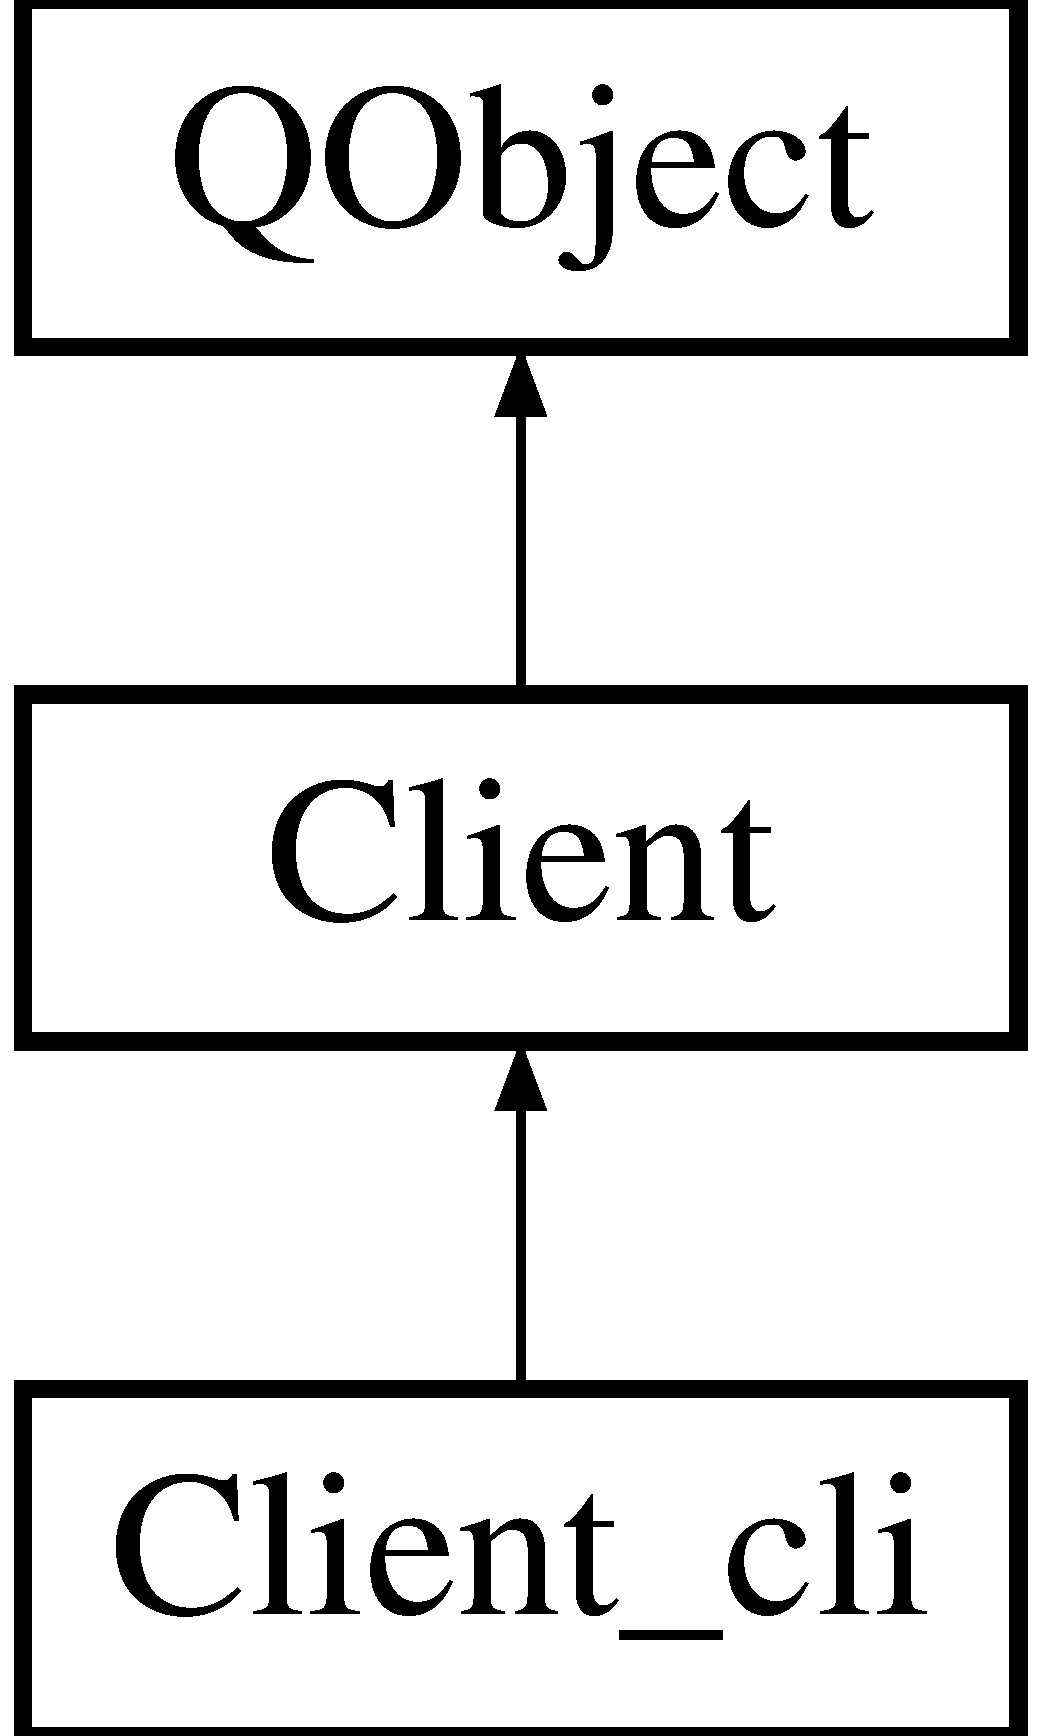
\includegraphics[height=3.000000cm]{classClient}
\end{center}
\end{figure}
\subsection*{Public Member Functions}
\begin{DoxyCompactItemize}
\item 
\hyperlink{classClient_a7832757f3fa37f564a21cb2b79b2baad}{Client} (Q\-Object $\ast$parent=0)
\item 
\hyperlink{classClient_a840e519ca781888cbd54181572ebe3a7}{$\sim$\-Client} ()
\item 
int \hyperlink{classClient_ac77cbaaec18851fcf9ab5bd58a90ef43}{send\-\_\-move} (std\-::string command)
\item 
int \hyperlink{classClient_a9e4a89c3937649327cceaf97e228c965}{accept\-\_\-state\-\_\-map} ()
\item 
int \hyperlink{classClient_ad3a29bf18762bd72c9362b71ac48956d}{connect\-\_\-socket} (const char $\ast$host)
\item 
int \hyperlink{classClient_ad7aad7d93ebed9931fa65b6c7eff32f5}{create\-\_\-game} (double \hyperlink{classClient_a37ec3a1f75d0ddcf25354b2bc552a039}{timeout}, int map\-\_\-type)
\item 
int \hyperlink{classClient_a0b123c350c7462456e4bb65109fc1578}{join\-\_\-game} (int game\-\_\-id)
\item 
int \hyperlink{classClient_a36a02d46f4bedcaa9ef9724e992cae60}{get\-\_\-games} ()
\item 
int \hyperlink{classClient_aaf73009df3d352ef47e282d0c65cb8e1}{show\-\_\-maps} ()
\end{DoxyCompactItemize}
\subsection*{Public Attributes}
\begin{DoxyCompactItemize}
\item 
int \hyperlink{classClient_ac6b50f30a11a753cabccc3f1fad83c82}{color}
\item 
int \hyperlink{classClient_a041ca02ff50a6544895c2e1013d29322}{pos\-\_\-x}
\item 
int \hyperlink{classClient_a1bf641e425b42c642a8be4d289a49229}{pos\-\_\-y}
\item 
int \hyperlink{classClient_aded73ce1e4c2d6a1f05c180956b85966}{width}
\item 
int \hyperlink{classClient_af7d6fce6b2b35773b4222cd8e86a840a}{height}
\item 
char \hyperlink{classClient_a6fcbb886abc984b5a6d590367e84d3f6}{map} \mbox{[}50\mbox{]}\mbox{[}50\mbox{]}
\item 
int \hyperlink{classClient_a8aa8ad037b45ef85ddc9d0b36bbb42b4}{time\-\_\-in\-\_\-game}
\item 
int \hyperlink{classClient_a60ac9a77128bfbcff9ae1dc7564fb441}{steps}
\item 
int \hyperlink{classClient_a70083e906d35591bd5e57612ce7a5786}{visit\-\_\-boxes}
\item 
std\-::string \hyperlink{classClient_aea5a7a7885c3bfd4dce194de2cef1003}{games}
\item 
std\-::string \hyperlink{classClient_a3ff1eaa556e62a485b2119d251d9d2d3}{maps}
\item 
double \hyperlink{classClient_a37ec3a1f75d0ddcf25354b2bc552a039}{timeout}
\end{DoxyCompactItemize}
\subsection*{Private Attributes}
\begin{DoxyCompactItemize}
\item 
Q\-Tcp\-Socket $\ast$ \hyperlink{classClient_aa684011b09c5d68ee677f026b036aaea}{client\-\_\-socket}
\end{DoxyCompactItemize}


\subsection{Detailed Description}
Umožňuje připojit klienta k serveru pomocí Q\-T \par
 Poslat serveru žádost o vytvoření nové hry \par
 Poslat žádost serveru o připojení se do již existující hry \par
 Zaslat serveru poslední tah, který se hráč chystá vykonat\par
 Přijmout změny posledního tahu hry\par
 Zobrazit všechny hry, k nimž je možnost se připojit a podrobnější informace k nim\par
 

\subsection{Constructor \& Destructor Documentation}
\hypertarget{classClient_a7832757f3fa37f564a21cb2b79b2baad}{\index{Client@{Client}!Client@{Client}}
\index{Client@{Client}!Client@{Client}}
\subsubsection[{Client}]{\setlength{\rightskip}{0pt plus 5cm}Client\-::\-Client (
\begin{DoxyParamCaption}
\item[{Q\-Object $\ast$}]{parent = {\ttfamily 0}}
\end{DoxyParamCaption}
)\hspace{0.3cm}{\ttfamily [explicit]}}}\label{classClient_a7832757f3fa37f564a21cb2b79b2baad}
\hypertarget{classClient_a840e519ca781888cbd54181572ebe3a7}{\index{Client@{Client}!$\sim$\-Client@{$\sim$\-Client}}
\index{$\sim$\-Client@{$\sim$\-Client}!Client@{Client}}
\subsubsection[{$\sim$\-Client}]{\setlength{\rightskip}{0pt plus 5cm}Client\-::$\sim$\-Client (
\begin{DoxyParamCaption}
{}
\end{DoxyParamCaption}
)}}\label{classClient_a840e519ca781888cbd54181572ebe3a7}


\subsection{Member Function Documentation}
\hypertarget{classClient_a9e4a89c3937649327cceaf97e228c965}{\index{Client@{Client}!accept\-\_\-state\-\_\-map@{accept\-\_\-state\-\_\-map}}
\index{accept\-\_\-state\-\_\-map@{accept\-\_\-state\-\_\-map}!Client@{Client}}
\subsubsection[{accept\-\_\-state\-\_\-map}]{\setlength{\rightskip}{0pt plus 5cm}int Client\-::accept\-\_\-state\-\_\-map (
\begin{DoxyParamCaption}
{}
\end{DoxyParamCaption}
)}}\label{classClient_a9e4a89c3937649327cceaf97e228c965}
Přečte ze socketu informace o aktuálním stavu hry a uloží je do atributu map \begin{DoxyReturn}{Returns}
1 pokud je konec hry, jinak nula 
\end{DoxyReturn}
\hypertarget{classClient_ad3a29bf18762bd72c9362b71ac48956d}{\index{Client@{Client}!connect\-\_\-socket@{connect\-\_\-socket}}
\index{connect\-\_\-socket@{connect\-\_\-socket}!Client@{Client}}
\subsubsection[{connect\-\_\-socket}]{\setlength{\rightskip}{0pt plus 5cm}int Client\-::connect\-\_\-socket (
\begin{DoxyParamCaption}
\item[{const char $\ast$}]{host}
\end{DoxyParamCaption}
)}}\label{classClient_ad3a29bf18762bd72c9362b71ac48956d}
Provede a zkontroluje připojení ke Q\-T socketu. 
\begin{DoxyParams}{Parameters}
{\em host} & Adresa, na kterou se připojuje client \\
\hline
\end{DoxyParams}
\begin{DoxyReturn}{Returns}
True, pokud se podaří připojit, jinak False 
\end{DoxyReturn}
\hypertarget{classClient_ad7aad7d93ebed9931fa65b6c7eff32f5}{\index{Client@{Client}!create\-\_\-game@{create\-\_\-game}}
\index{create\-\_\-game@{create\-\_\-game}!Client@{Client}}
\subsubsection[{create\-\_\-game}]{\setlength{\rightskip}{0pt plus 5cm}int Client\-::create\-\_\-game (
\begin{DoxyParamCaption}
\item[{double}]{timeout, }
\item[{int}]{map\-\_\-type}
\end{DoxyParamCaption}
)}}\label{classClient_ad7aad7d93ebed9931fa65b6c7eff32f5}
Pošle serveru žádost o vytvoření nové hry 
\begin{DoxyParams}{Parameters}
{\em width} & Šířka v počtech hracích políček (omezeno na 20-\/50). V případě nedodržení limitu velikosti dojde k vyvolání vyjímky \\
\hline
{\em height} & Výška programu, stejný limit i reakce na jeho nedodržení jako u width \\
\hline
{\em timeout} & Časový interval, ve kterém dochází ke změnám ve hře \\
\hline
\end{DoxyParams}
\begin{DoxyReturn}{Returns}
True (různé od 0) pokud se podařilo vytvořit hru, jinak False 
\end{DoxyReturn}
\hypertarget{classClient_a36a02d46f4bedcaa9ef9724e992cae60}{\index{Client@{Client}!get\-\_\-games@{get\-\_\-games}}
\index{get\-\_\-games@{get\-\_\-games}!Client@{Client}}
\subsubsection[{get\-\_\-games}]{\setlength{\rightskip}{0pt plus 5cm}int Client\-::get\-\_\-games (
\begin{DoxyParamCaption}
{}
\end{DoxyParamCaption}
)}}\label{classClient_a36a02d46f4bedcaa9ef9724e992cae60}
\hypertarget{classClient_a0b123c350c7462456e4bb65109fc1578}{\index{Client@{Client}!join\-\_\-game@{join\-\_\-game}}
\index{join\-\_\-game@{join\-\_\-game}!Client@{Client}}
\subsubsection[{join\-\_\-game}]{\setlength{\rightskip}{0pt plus 5cm}int Client\-::join\-\_\-game (
\begin{DoxyParamCaption}
\item[{int}]{game\-\_\-id}
\end{DoxyParamCaption}
)}}\label{classClient_a0b123c350c7462456e4bb65109fc1578}
Pošle serveru žádost o připojení do hry 
\begin{DoxyParams}{Parameters}
{\em game\-\_\-id} & Unikátní identifikátor hry generovaný serverem \\
\hline
\end{DoxyParams}
\begin{DoxyReturn}{Returns}
True, pokud nedojde k vyvolání výjimky 
\end{DoxyReturn}
\hypertarget{classClient_ac77cbaaec18851fcf9ab5bd58a90ef43}{\index{Client@{Client}!send\-\_\-move@{send\-\_\-move}}
\index{send\-\_\-move@{send\-\_\-move}!Client@{Client}}
\subsubsection[{send\-\_\-move}]{\setlength{\rightskip}{0pt plus 5cm}int Client\-::send\-\_\-move (
\begin{DoxyParamCaption}
\item[{std\-::string}]{command}
\end{DoxyParamCaption}
)}}\label{classClient_ac77cbaaec18851fcf9ab5bd58a90ef43}
Pošle serveru informaci o aktuálním tahu hráče 
\begin{DoxyParams}{Parameters}
{\em std\-::string} & command Příkaz reprezentující tah (go,right,left,stop,take,open) \\
\hline
\end{DoxyParams}
\begin{DoxyReturn}{Returns}
True, pokud nedojde k vyvolání výjimky 
\end{DoxyReturn}
\hypertarget{classClient_aaf73009df3d352ef47e282d0c65cb8e1}{\index{Client@{Client}!show\-\_\-maps@{show\-\_\-maps}}
\index{show\-\_\-maps@{show\-\_\-maps}!Client@{Client}}
\subsubsection[{show\-\_\-maps}]{\setlength{\rightskip}{0pt plus 5cm}int Client\-::show\-\_\-maps (
\begin{DoxyParamCaption}
{}
\end{DoxyParamCaption}
)}}\label{classClient_aaf73009df3d352ef47e282d0c65cb8e1}


\subsection{Member Data Documentation}
\hypertarget{classClient_aa684011b09c5d68ee677f026b036aaea}{\index{Client@{Client}!client\-\_\-socket@{client\-\_\-socket}}
\index{client\-\_\-socket@{client\-\_\-socket}!Client@{Client}}
\subsubsection[{client\-\_\-socket}]{\setlength{\rightskip}{0pt plus 5cm}Q\-Tcp\-Socket$\ast$ Client\-::client\-\_\-socket\hspace{0.3cm}{\ttfamily [private]}}}\label{classClient_aa684011b09c5d68ee677f026b036aaea}
\hypertarget{classClient_ac6b50f30a11a753cabccc3f1fad83c82}{\index{Client@{Client}!color@{color}}
\index{color@{color}!Client@{Client}}
\subsubsection[{color}]{\setlength{\rightskip}{0pt plus 5cm}int Client\-::color}}\label{classClient_ac6b50f30a11a753cabccc3f1fad83c82}
\hypertarget{classClient_aea5a7a7885c3bfd4dce194de2cef1003}{\index{Client@{Client}!games@{games}}
\index{games@{games}!Client@{Client}}
\subsubsection[{games}]{\setlength{\rightskip}{0pt plus 5cm}std\-::string Client\-::games}}\label{classClient_aea5a7a7885c3bfd4dce194de2cef1003}
\hypertarget{classClient_af7d6fce6b2b35773b4222cd8e86a840a}{\index{Client@{Client}!height@{height}}
\index{height@{height}!Client@{Client}}
\subsubsection[{height}]{\setlength{\rightskip}{0pt plus 5cm}int Client\-::height}}\label{classClient_af7d6fce6b2b35773b4222cd8e86a840a}
\hypertarget{classClient_a6fcbb886abc984b5a6d590367e84d3f6}{\index{Client@{Client}!map@{map}}
\index{map@{map}!Client@{Client}}
\subsubsection[{map}]{\setlength{\rightskip}{0pt plus 5cm}char Client\-::map\mbox{[}50\mbox{]}\mbox{[}50\mbox{]}}}\label{classClient_a6fcbb886abc984b5a6d590367e84d3f6}
\hypertarget{classClient_a3ff1eaa556e62a485b2119d251d9d2d3}{\index{Client@{Client}!maps@{maps}}
\index{maps@{maps}!Client@{Client}}
\subsubsection[{maps}]{\setlength{\rightskip}{0pt plus 5cm}std\-::string Client\-::maps}}\label{classClient_a3ff1eaa556e62a485b2119d251d9d2d3}
\hypertarget{classClient_a041ca02ff50a6544895c2e1013d29322}{\index{Client@{Client}!pos\-\_\-x@{pos\-\_\-x}}
\index{pos\-\_\-x@{pos\-\_\-x}!Client@{Client}}
\subsubsection[{pos\-\_\-x}]{\setlength{\rightskip}{0pt plus 5cm}int Client\-::pos\-\_\-x}}\label{classClient_a041ca02ff50a6544895c2e1013d29322}
\hypertarget{classClient_a1bf641e425b42c642a8be4d289a49229}{\index{Client@{Client}!pos\-\_\-y@{pos\-\_\-y}}
\index{pos\-\_\-y@{pos\-\_\-y}!Client@{Client}}
\subsubsection[{pos\-\_\-y}]{\setlength{\rightskip}{0pt plus 5cm}int Client\-::pos\-\_\-y}}\label{classClient_a1bf641e425b42c642a8be4d289a49229}
\hypertarget{classClient_a60ac9a77128bfbcff9ae1dc7564fb441}{\index{Client@{Client}!steps@{steps}}
\index{steps@{steps}!Client@{Client}}
\subsubsection[{steps}]{\setlength{\rightskip}{0pt plus 5cm}int Client\-::steps}}\label{classClient_a60ac9a77128bfbcff9ae1dc7564fb441}
\hypertarget{classClient_a8aa8ad037b45ef85ddc9d0b36bbb42b4}{\index{Client@{Client}!time\-\_\-in\-\_\-game@{time\-\_\-in\-\_\-game}}
\index{time\-\_\-in\-\_\-game@{time\-\_\-in\-\_\-game}!Client@{Client}}
\subsubsection[{time\-\_\-in\-\_\-game}]{\setlength{\rightskip}{0pt plus 5cm}int Client\-::time\-\_\-in\-\_\-game}}\label{classClient_a8aa8ad037b45ef85ddc9d0b36bbb42b4}
\hypertarget{classClient_a37ec3a1f75d0ddcf25354b2bc552a039}{\index{Client@{Client}!timeout@{timeout}}
\index{timeout@{timeout}!Client@{Client}}
\subsubsection[{timeout}]{\setlength{\rightskip}{0pt plus 5cm}double Client\-::timeout}}\label{classClient_a37ec3a1f75d0ddcf25354b2bc552a039}
\hypertarget{classClient_a70083e906d35591bd5e57612ce7a5786}{\index{Client@{Client}!visit\-\_\-boxes@{visit\-\_\-boxes}}
\index{visit\-\_\-boxes@{visit\-\_\-boxes}!Client@{Client}}
\subsubsection[{visit\-\_\-boxes}]{\setlength{\rightskip}{0pt plus 5cm}int Client\-::visit\-\_\-boxes}}\label{classClient_a70083e906d35591bd5e57612ce7a5786}
\hypertarget{classClient_aded73ce1e4c2d6a1f05c180956b85966}{\index{Client@{Client}!width@{width}}
\index{width@{width}!Client@{Client}}
\subsubsection[{width}]{\setlength{\rightskip}{0pt plus 5cm}int Client\-::width}}\label{classClient_aded73ce1e4c2d6a1f05c180956b85966}


The documentation for this class was generated from the following files\-:\begin{DoxyCompactItemize}
\item 
\hyperlink{client_8h}{client.\-h}\item 
\hyperlink{client_8cpp}{client.\-cpp}\end{DoxyCompactItemize}

\hypertarget{classClient__cli}{\section{Client\-\_\-cli Class Reference}
\label{classClient__cli}\index{Client\-\_\-cli@{Client\-\_\-cli}}
}


{\ttfamily \#include $<$client\-\_\-cli.\-h$>$}

Inheritance diagram for Client\-\_\-cli\-:\begin{figure}[H]
\begin{center}
\leavevmode
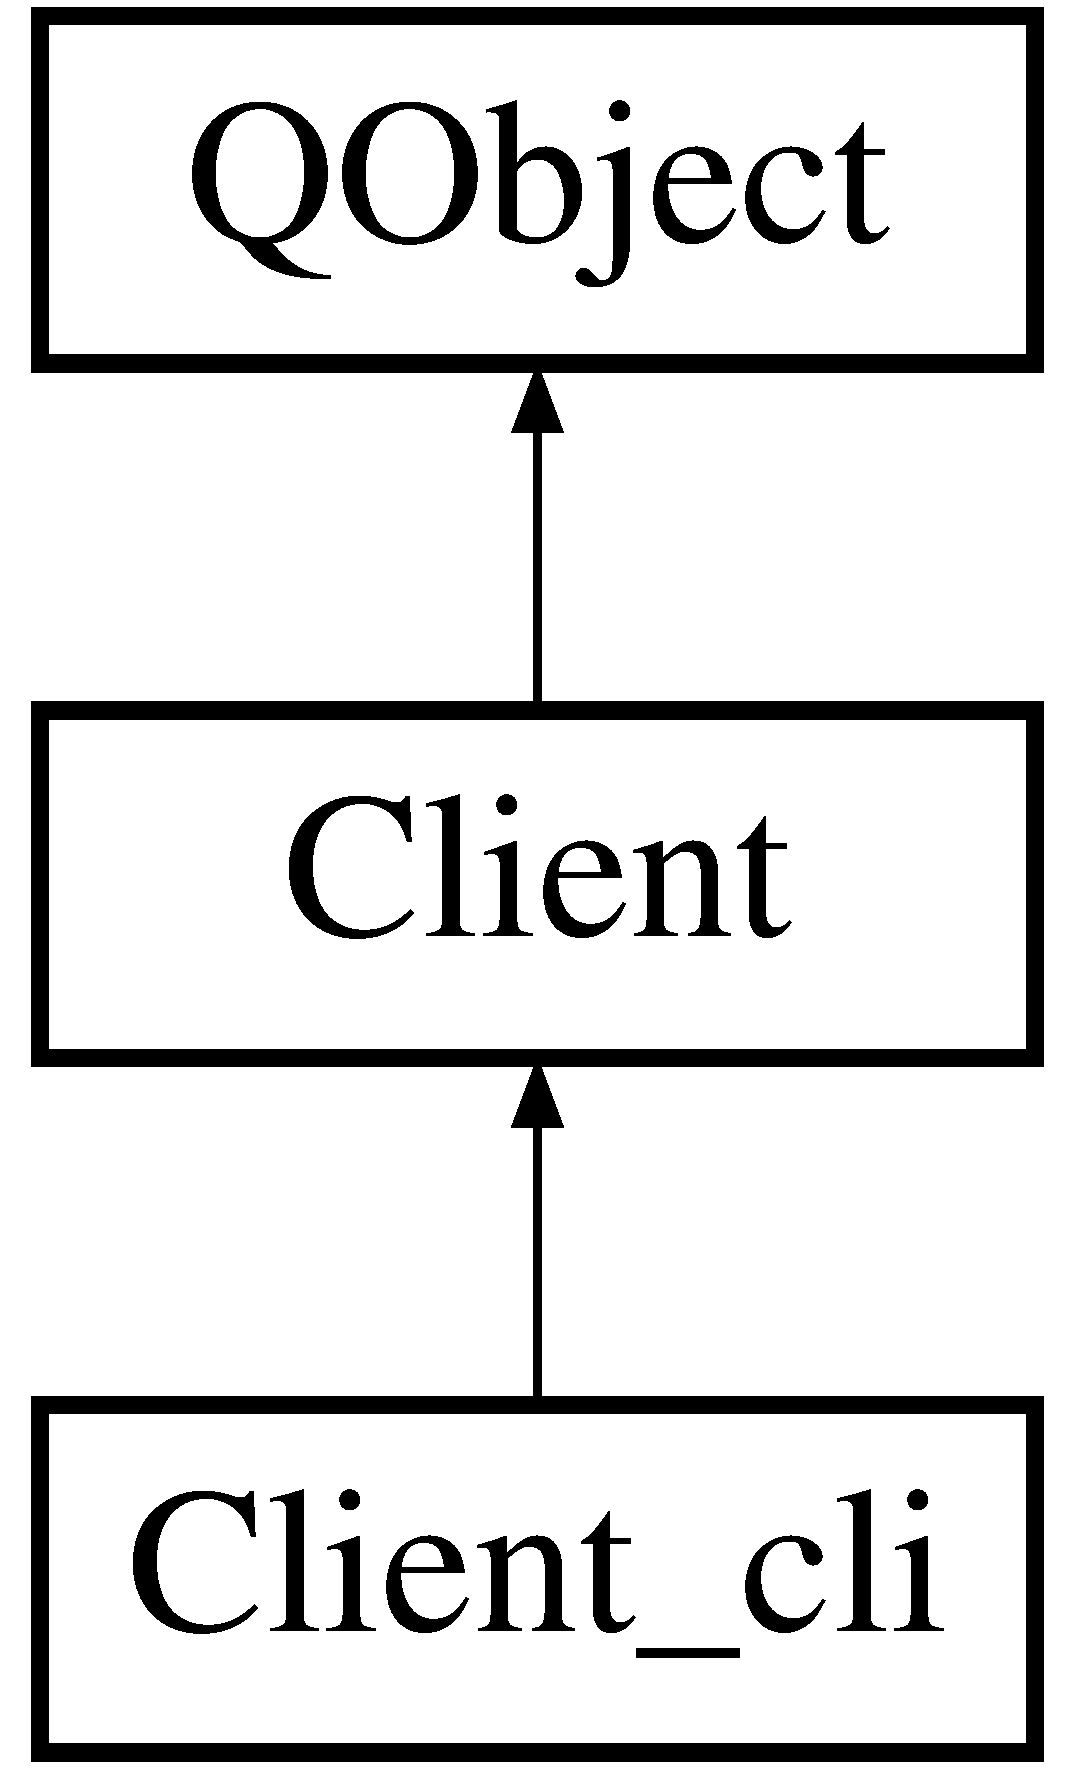
\includegraphics[height=3.000000cm]{classClient__cli}
\end{center}
\end{figure}
\subsection*{Public Member Functions}
\begin{DoxyCompactItemize}
\item 
void \hyperlink{classClient__cli_aab3857cbd9c35a5b75ad01983c43ef9d}{print\-\_\-map} ()
\item 
void \hyperlink{classClient__cli_acb41c82bae07ce96591a189cbd5d6482}{print\-\_\-games} ()
\item 
void \hyperlink{classClient__cli_a3013ba30eb58163516088a649abc878f}{print\-\_\-maps} ()
\item 
\hyperlink{classClient__cli_a60327af92733d8c08caf4461cc183700}{Client\-\_\-cli} ()
\item 
\hyperlink{classClient__cli_a8c6fc3daf73356dffc52a9429c093b64}{$\sim$\-Client\-\_\-cli} ()
\end{DoxyCompactItemize}
\subsection*{Additional Inherited Members}


\subsection{Detailed Description}
Rozšiřuje třídu \hyperlink{classClient}{Client} o metody výpisu na konzoli pro konzolovou verzi hry. 

\subsection{Constructor \& Destructor Documentation}
\hypertarget{classClient__cli_a60327af92733d8c08caf4461cc183700}{\index{Client\-\_\-cli@{Client\-\_\-cli}!Client\-\_\-cli@{Client\-\_\-cli}}
\index{Client\-\_\-cli@{Client\-\_\-cli}!Client_cli@{Client\-\_\-cli}}
\subsubsection[{Client\-\_\-cli}]{\setlength{\rightskip}{0pt plus 5cm}Client\-\_\-cli\-::\-Client\-\_\-cli (
\begin{DoxyParamCaption}
{}
\end{DoxyParamCaption}
)}}\label{classClient__cli_a60327af92733d8c08caf4461cc183700}
\hypertarget{classClient__cli_a8c6fc3daf73356dffc52a9429c093b64}{\index{Client\-\_\-cli@{Client\-\_\-cli}!$\sim$\-Client\-\_\-cli@{$\sim$\-Client\-\_\-cli}}
\index{$\sim$\-Client\-\_\-cli@{$\sim$\-Client\-\_\-cli}!Client_cli@{Client\-\_\-cli}}
\subsubsection[{$\sim$\-Client\-\_\-cli}]{\setlength{\rightskip}{0pt plus 5cm}Client\-\_\-cli\-::$\sim$\-Client\-\_\-cli (
\begin{DoxyParamCaption}
{}
\end{DoxyParamCaption}
)}}\label{classClient__cli_a8c6fc3daf73356dffc52a9429c093b64}


\subsection{Member Function Documentation}
\hypertarget{classClient__cli_acb41c82bae07ce96591a189cbd5d6482}{\index{Client\-\_\-cli@{Client\-\_\-cli}!print\-\_\-games@{print\-\_\-games}}
\index{print\-\_\-games@{print\-\_\-games}!Client_cli@{Client\-\_\-cli}}
\subsubsection[{print\-\_\-games}]{\setlength{\rightskip}{0pt plus 5cm}void Client\-\_\-cli\-::print\-\_\-games (
\begin{DoxyParamCaption}
{}
\end{DoxyParamCaption}
)}}\label{classClient__cli_acb41c82bae07ce96591a189cbd5d6482}
Vypíše rozehrané hry, ke kterým se lze připojit \hypertarget{classClient__cli_aab3857cbd9c35a5b75ad01983c43ef9d}{\index{Client\-\_\-cli@{Client\-\_\-cli}!print\-\_\-map@{print\-\_\-map}}
\index{print\-\_\-map@{print\-\_\-map}!Client_cli@{Client\-\_\-cli}}
\subsubsection[{print\-\_\-map}]{\setlength{\rightskip}{0pt plus 5cm}void Client\-\_\-cli\-::print\-\_\-map (
\begin{DoxyParamCaption}
{}
\end{DoxyParamCaption}
)}}\label{classClient__cli_aab3857cbd9c35a5b75ad01983c43ef9d}
Vypíše stav hrací plochy \hypertarget{classClient__cli_a3013ba30eb58163516088a649abc878f}{\index{Client\-\_\-cli@{Client\-\_\-cli}!print\-\_\-maps@{print\-\_\-maps}}
\index{print\-\_\-maps@{print\-\_\-maps}!Client_cli@{Client\-\_\-cli}}
\subsubsection[{print\-\_\-maps}]{\setlength{\rightskip}{0pt plus 5cm}void Client\-\_\-cli\-::print\-\_\-maps (
\begin{DoxyParamCaption}
{}
\end{DoxyParamCaption}
)}}\label{classClient__cli_a3013ba30eb58163516088a649abc878f}
Vypíše mapy, které jsou k dispozici pro založení nové hry 

The documentation for this class was generated from the following files\-:\begin{DoxyCompactItemize}
\item 
\hyperlink{client__cli_8h}{client\-\_\-cli.\-h}\item 
\hyperlink{client__cli_8cpp}{client\-\_\-cli.\-cpp}\end{DoxyCompactItemize}

\hypertarget{classErrors}{\section{Errors Class Reference}
\label{classErrors}\index{Errors@{Errors}}
}


{\ttfamily \#include $<$errors.\-h$>$}

Inheritance diagram for Errors\-:\begin{figure}[H]
\begin{center}
\leavevmode
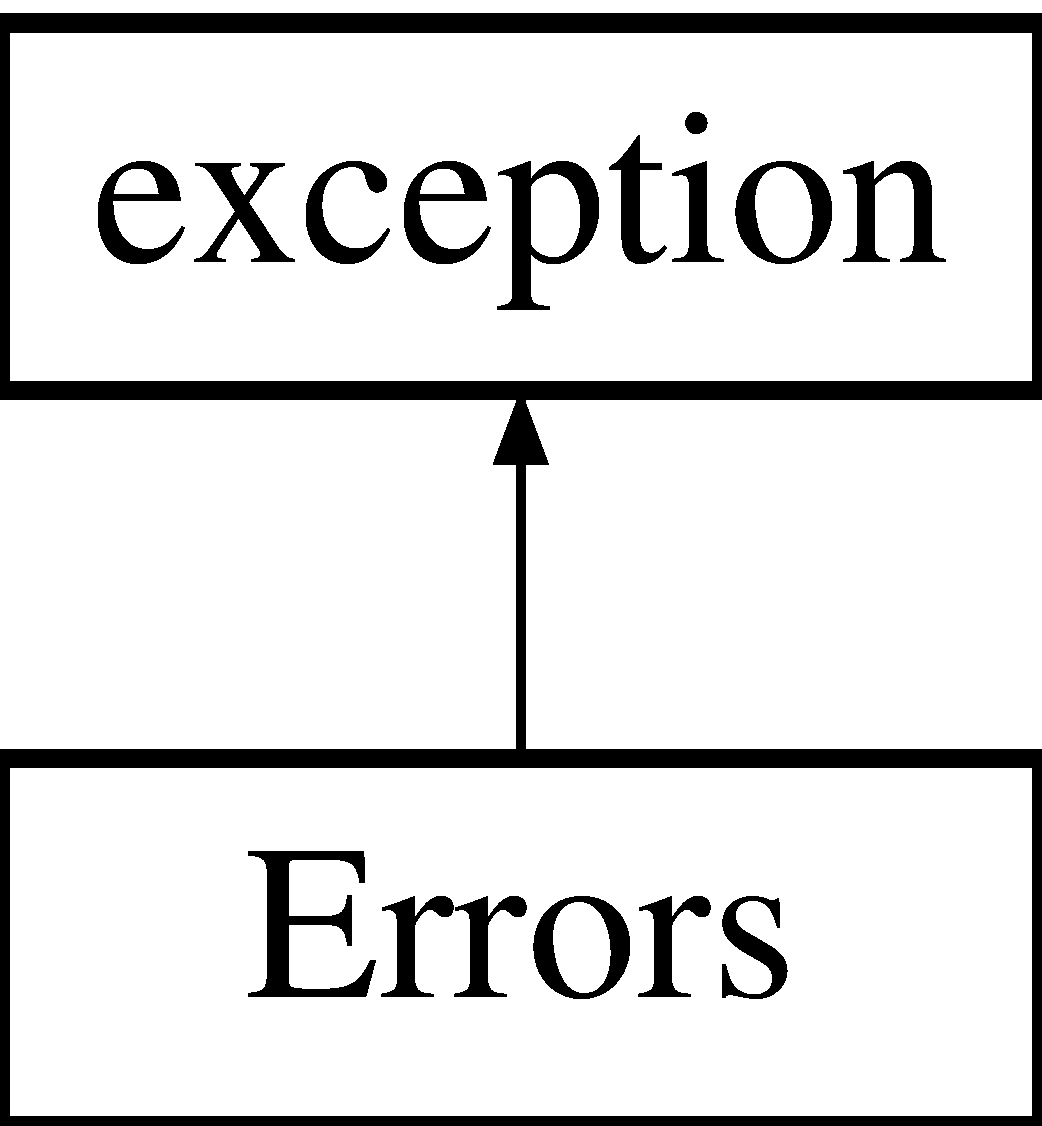
\includegraphics[height=2.000000cm]{classErrors}
\end{center}
\end{figure}
\subsection*{Public Types}
\begin{DoxyCompactItemize}
\item 
enum \hyperlink{classErrors_a93a0cc4db45d07a1395a8eaa9c39caf4}{error\-\_\-codes} \{ \\*
\hyperlink{classErrors_a93a0cc4db45d07a1395a8eaa9c39caf4ad367a96807f95dce493f81fedda82a15}{S\-O\-C\-K\-E\-T\-\_\-\-C\-O\-N\-N\-E\-C\-T}, 
\hyperlink{classErrors_a93a0cc4db45d07a1395a8eaa9c39caf4a62d04313dce718fbab4bf2d1ba40231e}{P\-A\-R\-A\-M\-\_\-\-E\-R\-R\-O\-R}, 
\hyperlink{classErrors_a93a0cc4db45d07a1395a8eaa9c39caf4a343a84847d2ea3da575fa80a35817e43}{B\-O\-X\-E\-S\-\_\-\-W\-I\-D\-T\-H}, 
\hyperlink{classErrors_a93a0cc4db45d07a1395a8eaa9c39caf4ad7dcb67868a667b1ab6ac60497f894c2}{B\-O\-X\-E\-S\-\_\-\-H\-E\-I\-G\-H\-T}, 
\\*
\hyperlink{classErrors_a93a0cc4db45d07a1395a8eaa9c39caf4a65c402720b8ae2b51cc905c7b596dc5d}{T\-I\-M\-E\-O\-U\-T}, 
\hyperlink{classErrors_a93a0cc4db45d07a1395a8eaa9c39caf4a3f4fcdb5424e1904051934ddba97fac6}{W\-R\-I\-T\-E\-\_\-\-S\-O\-C\-K\-E\-T}, 
\hyperlink{classErrors_a93a0cc4db45d07a1395a8eaa9c39caf4a35377db2acec293b3bc0f1f619009755}{S\-O\-C\-K\-E\-T\-\_\-\-R\-E\-A\-D}, 
\hyperlink{classErrors_a93a0cc4db45d07a1395a8eaa9c39caf4a7ae24fb4b67f13832aa78399563b4ba4}{G\-A\-M\-E\-\_\-\-N\-O\-T\-\_\-\-C\-R\-E\-A\-T\-E\-D}, 
\\*
\hyperlink{classErrors_a93a0cc4db45d07a1395a8eaa9c39caf4a098463bf2ad00a4735b1defd0d8cd121}{N\-O\-T\-\_\-\-J\-O\-I\-N\-E\-D}, 
\hyperlink{classErrors_a93a0cc4db45d07a1395a8eaa9c39caf4af5d508f9d3ac0c6d7abefce1c151c075}{U\-N\-K\-N\-O\-W\-N\-\_\-\-C\-O\-M\-M\-A\-N\-D}
 \}
\end{DoxyCompactItemize}
\subsection*{Public Member Functions}
\begin{DoxyCompactItemize}
\item 
\hyperlink{classErrors_a3a2481d800ce1b4000995ba0005613e9}{Errors} (int \hyperlink{classErrors_ab886b164554b2094ff8263917cfcaaae}{code})
\item 
std\-::string \hyperlink{classErrors_afed158318501890c617c04a9ec2aa9f4}{get\-\_\-message} ()
\end{DoxyCompactItemize}
\subsection*{Public Attributes}
\begin{DoxyCompactItemize}
\item 
int \hyperlink{classErrors_ab886b164554b2094ff8263917cfcaaae}{code}
\item 
std\-::string \hyperlink{classErrors_abce2313e24596b78f074bc3a31ae5dab}{error\-\_\-messages} \mbox{[}10\mbox{]}
\end{DoxyCompactItemize}


\subsection{Detailed Description}
Třída je potomkem třídy exception, kterou rozšiřuje o nové výjimky, které mohou vzniknout v průběhu aplikace bludiště 

\subsection{Member Enumeration Documentation}
\hypertarget{classErrors_a93a0cc4db45d07a1395a8eaa9c39caf4}{\index{Errors@{Errors}!error\-\_\-codes@{error\-\_\-codes}}
\index{error\-\_\-codes@{error\-\_\-codes}!Errors@{Errors}}
\subsubsection[{error\-\_\-codes}]{\setlength{\rightskip}{0pt plus 5cm}enum {\bf Errors\-::error\-\_\-codes}}}\label{classErrors_a93a0cc4db45d07a1395a8eaa9c39caf4}
Enumerátor chybových kódů \begin{Desc}
\item[Enumerator]\par
\begin{description}
\index{S\-O\-C\-K\-E\-T\-\_\-\-C\-O\-N\-N\-E\-C\-T@{S\-O\-C\-K\-E\-T\-\_\-\-C\-O\-N\-N\-E\-C\-T}!Errors@{Errors}}\index{Errors@{Errors}!S\-O\-C\-K\-E\-T\-\_\-\-C\-O\-N\-N\-E\-C\-T@{S\-O\-C\-K\-E\-T\-\_\-\-C\-O\-N\-N\-E\-C\-T}}\item[{\em 
\hypertarget{classErrors_a93a0cc4db45d07a1395a8eaa9c39caf4ad367a96807f95dce493f81fedda82a15}{S\-O\-C\-K\-E\-T\-\_\-\-C\-O\-N\-N\-E\-C\-T}\label{classErrors_a93a0cc4db45d07a1395a8eaa9c39caf4ad367a96807f95dce493f81fedda82a15}
}]\index{P\-A\-R\-A\-M\-\_\-\-E\-R\-R\-O\-R@{P\-A\-R\-A\-M\-\_\-\-E\-R\-R\-O\-R}!Errors@{Errors}}\index{Errors@{Errors}!P\-A\-R\-A\-M\-\_\-\-E\-R\-R\-O\-R@{P\-A\-R\-A\-M\-\_\-\-E\-R\-R\-O\-R}}\item[{\em 
\hypertarget{classErrors_a93a0cc4db45d07a1395a8eaa9c39caf4a62d04313dce718fbab4bf2d1ba40231e}{P\-A\-R\-A\-M\-\_\-\-E\-R\-R\-O\-R}\label{classErrors_a93a0cc4db45d07a1395a8eaa9c39caf4a62d04313dce718fbab4bf2d1ba40231e}
}]\index{B\-O\-X\-E\-S\-\_\-\-W\-I\-D\-T\-H@{B\-O\-X\-E\-S\-\_\-\-W\-I\-D\-T\-H}!Errors@{Errors}}\index{Errors@{Errors}!B\-O\-X\-E\-S\-\_\-\-W\-I\-D\-T\-H@{B\-O\-X\-E\-S\-\_\-\-W\-I\-D\-T\-H}}\item[{\em 
\hypertarget{classErrors_a93a0cc4db45d07a1395a8eaa9c39caf4a343a84847d2ea3da575fa80a35817e43}{B\-O\-X\-E\-S\-\_\-\-W\-I\-D\-T\-H}\label{classErrors_a93a0cc4db45d07a1395a8eaa9c39caf4a343a84847d2ea3da575fa80a35817e43}
}]\index{B\-O\-X\-E\-S\-\_\-\-H\-E\-I\-G\-H\-T@{B\-O\-X\-E\-S\-\_\-\-H\-E\-I\-G\-H\-T}!Errors@{Errors}}\index{Errors@{Errors}!B\-O\-X\-E\-S\-\_\-\-H\-E\-I\-G\-H\-T@{B\-O\-X\-E\-S\-\_\-\-H\-E\-I\-G\-H\-T}}\item[{\em 
\hypertarget{classErrors_a93a0cc4db45d07a1395a8eaa9c39caf4ad7dcb67868a667b1ab6ac60497f894c2}{B\-O\-X\-E\-S\-\_\-\-H\-E\-I\-G\-H\-T}\label{classErrors_a93a0cc4db45d07a1395a8eaa9c39caf4ad7dcb67868a667b1ab6ac60497f894c2}
}]\index{T\-I\-M\-E\-O\-U\-T@{T\-I\-M\-E\-O\-U\-T}!Errors@{Errors}}\index{Errors@{Errors}!T\-I\-M\-E\-O\-U\-T@{T\-I\-M\-E\-O\-U\-T}}\item[{\em 
\hypertarget{classErrors_a93a0cc4db45d07a1395a8eaa9c39caf4a65c402720b8ae2b51cc905c7b596dc5d}{T\-I\-M\-E\-O\-U\-T}\label{classErrors_a93a0cc4db45d07a1395a8eaa9c39caf4a65c402720b8ae2b51cc905c7b596dc5d}
}]\index{W\-R\-I\-T\-E\-\_\-\-S\-O\-C\-K\-E\-T@{W\-R\-I\-T\-E\-\_\-\-S\-O\-C\-K\-E\-T}!Errors@{Errors}}\index{Errors@{Errors}!W\-R\-I\-T\-E\-\_\-\-S\-O\-C\-K\-E\-T@{W\-R\-I\-T\-E\-\_\-\-S\-O\-C\-K\-E\-T}}\item[{\em 
\hypertarget{classErrors_a93a0cc4db45d07a1395a8eaa9c39caf4a3f4fcdb5424e1904051934ddba97fac6}{W\-R\-I\-T\-E\-\_\-\-S\-O\-C\-K\-E\-T}\label{classErrors_a93a0cc4db45d07a1395a8eaa9c39caf4a3f4fcdb5424e1904051934ddba97fac6}
}]\index{S\-O\-C\-K\-E\-T\-\_\-\-R\-E\-A\-D@{S\-O\-C\-K\-E\-T\-\_\-\-R\-E\-A\-D}!Errors@{Errors}}\index{Errors@{Errors}!S\-O\-C\-K\-E\-T\-\_\-\-R\-E\-A\-D@{S\-O\-C\-K\-E\-T\-\_\-\-R\-E\-A\-D}}\item[{\em 
\hypertarget{classErrors_a93a0cc4db45d07a1395a8eaa9c39caf4a35377db2acec293b3bc0f1f619009755}{S\-O\-C\-K\-E\-T\-\_\-\-R\-E\-A\-D}\label{classErrors_a93a0cc4db45d07a1395a8eaa9c39caf4a35377db2acec293b3bc0f1f619009755}
}]\index{G\-A\-M\-E\-\_\-\-N\-O\-T\-\_\-\-C\-R\-E\-A\-T\-E\-D@{G\-A\-M\-E\-\_\-\-N\-O\-T\-\_\-\-C\-R\-E\-A\-T\-E\-D}!Errors@{Errors}}\index{Errors@{Errors}!G\-A\-M\-E\-\_\-\-N\-O\-T\-\_\-\-C\-R\-E\-A\-T\-E\-D@{G\-A\-M\-E\-\_\-\-N\-O\-T\-\_\-\-C\-R\-E\-A\-T\-E\-D}}\item[{\em 
\hypertarget{classErrors_a93a0cc4db45d07a1395a8eaa9c39caf4a7ae24fb4b67f13832aa78399563b4ba4}{G\-A\-M\-E\-\_\-\-N\-O\-T\-\_\-\-C\-R\-E\-A\-T\-E\-D}\label{classErrors_a93a0cc4db45d07a1395a8eaa9c39caf4a7ae24fb4b67f13832aa78399563b4ba4}
}]\index{N\-O\-T\-\_\-\-J\-O\-I\-N\-E\-D@{N\-O\-T\-\_\-\-J\-O\-I\-N\-E\-D}!Errors@{Errors}}\index{Errors@{Errors}!N\-O\-T\-\_\-\-J\-O\-I\-N\-E\-D@{N\-O\-T\-\_\-\-J\-O\-I\-N\-E\-D}}\item[{\em 
\hypertarget{classErrors_a93a0cc4db45d07a1395a8eaa9c39caf4a098463bf2ad00a4735b1defd0d8cd121}{N\-O\-T\-\_\-\-J\-O\-I\-N\-E\-D}\label{classErrors_a93a0cc4db45d07a1395a8eaa9c39caf4a098463bf2ad00a4735b1defd0d8cd121}
}]\index{U\-N\-K\-N\-O\-W\-N\-\_\-\-C\-O\-M\-M\-A\-N\-D@{U\-N\-K\-N\-O\-W\-N\-\_\-\-C\-O\-M\-M\-A\-N\-D}!Errors@{Errors}}\index{Errors@{Errors}!U\-N\-K\-N\-O\-W\-N\-\_\-\-C\-O\-M\-M\-A\-N\-D@{U\-N\-K\-N\-O\-W\-N\-\_\-\-C\-O\-M\-M\-A\-N\-D}}\item[{\em 
\hypertarget{classErrors_a93a0cc4db45d07a1395a8eaa9c39caf4af5d508f9d3ac0c6d7abefce1c151c075}{U\-N\-K\-N\-O\-W\-N\-\_\-\-C\-O\-M\-M\-A\-N\-D}\label{classErrors_a93a0cc4db45d07a1395a8eaa9c39caf4af5d508f9d3ac0c6d7abefce1c151c075}
}]\end{description}
\end{Desc}


\subsection{Constructor \& Destructor Documentation}
\hypertarget{classErrors_a3a2481d800ce1b4000995ba0005613e9}{\index{Errors@{Errors}!Errors@{Errors}}
\index{Errors@{Errors}!Errors@{Errors}}
\subsubsection[{Errors}]{\setlength{\rightskip}{0pt plus 5cm}Errors\-::\-Errors (
\begin{DoxyParamCaption}
\item[{int}]{code}
\end{DoxyParamCaption}
)}}\label{classErrors_a3a2481d800ce1b4000995ba0005613e9}


\subsection{Member Function Documentation}
\hypertarget{classErrors_afed158318501890c617c04a9ec2aa9f4}{\index{Errors@{Errors}!get\-\_\-message@{get\-\_\-message}}
\index{get\-\_\-message@{get\-\_\-message}!Errors@{Errors}}
\subsubsection[{get\-\_\-message}]{\setlength{\rightskip}{0pt plus 5cm}std\-::string Errors\-::get\-\_\-message (
\begin{DoxyParamCaption}
{}
\end{DoxyParamCaption}
)}}\label{classErrors_afed158318501890c617c04a9ec2aa9f4}
\begin{DoxyReturn}{Returns}
Chybovou hlášku vyjímky, která byla vyvolána 
\end{DoxyReturn}


\subsection{Member Data Documentation}
\hypertarget{classErrors_ab886b164554b2094ff8263917cfcaaae}{\index{Errors@{Errors}!code@{code}}
\index{code@{code}!Errors@{Errors}}
\subsubsection[{code}]{\setlength{\rightskip}{0pt plus 5cm}int Errors\-::code}}\label{classErrors_ab886b164554b2094ff8263917cfcaaae}
\hypertarget{classErrors_abce2313e24596b78f074bc3a31ae5dab}{\index{Errors@{Errors}!error\-\_\-messages@{error\-\_\-messages}}
\index{error\-\_\-messages@{error\-\_\-messages}!Errors@{Errors}}
\subsubsection[{error\-\_\-messages}]{\setlength{\rightskip}{0pt plus 5cm}std\-::string Errors\-::error\-\_\-messages\mbox{[}10\mbox{]}}}\label{classErrors_abce2313e24596b78f074bc3a31ae5dab}
{\bfseries Initial value\-:}
\begin{DoxyCode}
=
    \{
        \textcolor{stringliteral}{"Nepodařilo se připojit k serveru"},
        \textcolor{stringliteral}{"Nebyl zadán správně parametr"},
        \textcolor{stringliteral}{"Špatná šířka hracího pole (nutno zadat 20 - 50)"},
        \textcolor{stringliteral}{"Špatná výška hracího pole (nutno zadat 20 - 50)"},
        \textcolor{stringliteral}{"Nepovolený časový interval změn (nutno zadat 0.5 - 5 sekund)"},
        \textcolor{stringliteral}{"Nepodařilo se odeslat data serveru"},   
        \textcolor{stringliteral}{"Nepodařilo se přijmout data od serveru"},
        \textcolor{stringliteral}{"Hru nebylo možné vytvořit, zkontrolujte, že jste serveru poslal správné informace"},
        \textcolor{stringliteral}{"Nepodařilo se vás připojit do hry"},
        \textcolor{stringliteral}{"Neznámý příkaz pro tah (použij: go,stop,left,right,take,open)"},
    \}
\end{DoxyCode}
Pole chybových hlášek 

The documentation for this class was generated from the following files\-:\begin{DoxyCompactItemize}
\item 
\hyperlink{errors_8h}{errors.\-h}\item 
\hyperlink{errors_8cpp}{errors.\-cpp}\end{DoxyCompactItemize}

\hypertarget{classGame__field}{\section{Game\-\_\-field Class Reference}
\label{classGame__field}\index{Game\-\_\-field@{Game\-\_\-field}}
}


{\ttfamily \#include $<$game\-\_\-field.\-h$>$}

Inheritance diagram for Game\-\_\-field\-:\begin{figure}[H]
\begin{center}
\leavevmode
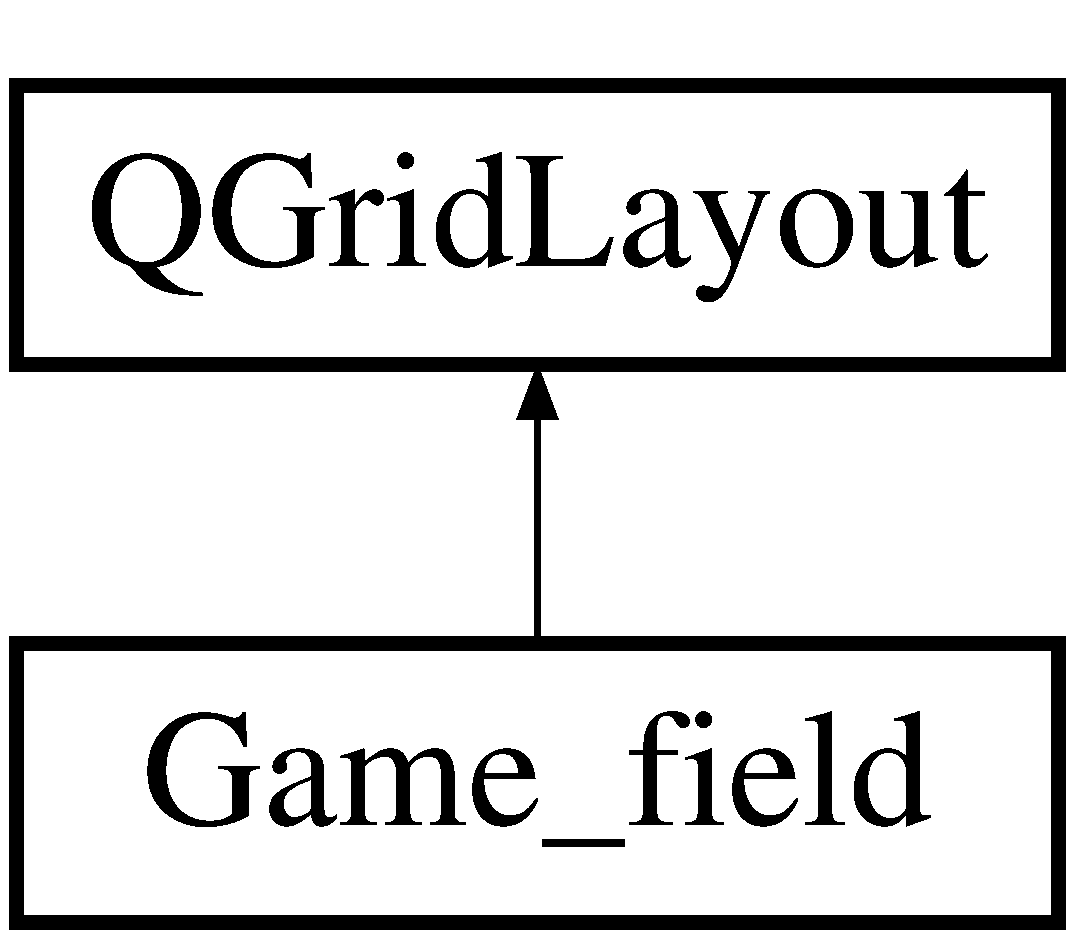
\includegraphics[height=2.000000cm]{classGame__field}
\end{center}
\end{figure}
\subsection*{Public Member Functions}
\begin{DoxyCompactItemize}
\item 
\hyperlink{classGame__field_ae0ab9fc16c3480706396bc866eacda71}{Game\-\_\-field} (int \hyperlink{classGame__field_a21f6f197950dc49b669faa6d90208912}{height}, int \hyperlink{classGame__field_aded6e31a0afaf905171e2a4b06a52e29}{width}, Q\-Widget $\ast$parent=0)
\item 
\hyperlink{classGame__field_a5372177f62cdd385680813be54d5e80f}{$\sim$\-Game\-\_\-field} ()
\item 
void \hyperlink{classGame__field_a9af443542dd34f1d13e08d9358a06a33}{set\-\_\-map} (char map\mbox{[}50\mbox{]}\mbox{[}50\mbox{]})
\end{DoxyCompactItemize}
\subsection*{Public Attributes}
\begin{DoxyCompactItemize}
\item 
Q\-Pixmap $\ast$ \hyperlink{classGame__field_ae9235aa8798fdb0db4385064b5c40b21}{empty}
\item 
Q\-Pixmap $\ast$ \hyperlink{classGame__field_aef92a0fbf4509d6b6bfa9f8833acdbb9}{monster\-\_\-up}
\item 
Q\-Pixmap $\ast$ \hyperlink{classGame__field_a7366baff6372c613d42616d7e0286fa0}{wall}
\item 
Q\-Pixmap $\ast$ \hyperlink{classGame__field_af81b72dc5a1da7aae4929bdd43c449bd}{white\-\_\-up}
\item 
Q\-Label $\ast$ \hyperlink{classGame__field_a144d007ae7c2224829dd34d67dd96e98}{field} \mbox{[}50\mbox{]}\mbox{[}50\mbox{]}
\item 
int \hyperlink{classGame__field_a21f6f197950dc49b669faa6d90208912}{height}
\item 
int \hyperlink{classGame__field_aded6e31a0afaf905171e2a4b06a52e29}{width}
\end{DoxyCompactItemize}


\subsection{Detailed Description}
Obsahuje všechny možné obrázky uložené v Q\-Pixmap, zobrazitelné na hrací ploše (hráče s natočením, hlídače s natočením, zeď, klíč, bránu). \par
 Obsahuje hrací plochu jako dvourozměrnou matici instancí třídy Q\-Label, na které se vykreslují příslušné obrázky uložené v instanci Q\-Pixmap. 

\subsection{Constructor \& Destructor Documentation}
\hypertarget{classGame__field_ae0ab9fc16c3480706396bc866eacda71}{\index{Game\-\_\-field@{Game\-\_\-field}!Game\-\_\-field@{Game\-\_\-field}}
\index{Game\-\_\-field@{Game\-\_\-field}!Game_field@{Game\-\_\-field}}
\subsubsection[{Game\-\_\-field}]{\setlength{\rightskip}{0pt plus 5cm}Game\-\_\-field\-::\-Game\-\_\-field (
\begin{DoxyParamCaption}
\item[{int}]{height, }
\item[{int}]{width, }
\item[{Q\-Widget $\ast$}]{parent = {\ttfamily 0}}
\end{DoxyParamCaption}
)}}\label{classGame__field_ae0ab9fc16c3480706396bc866eacda71}
\hypertarget{classGame__field_a5372177f62cdd385680813be54d5e80f}{\index{Game\-\_\-field@{Game\-\_\-field}!$\sim$\-Game\-\_\-field@{$\sim$\-Game\-\_\-field}}
\index{$\sim$\-Game\-\_\-field@{$\sim$\-Game\-\_\-field}!Game_field@{Game\-\_\-field}}
\subsubsection[{$\sim$\-Game\-\_\-field}]{\setlength{\rightskip}{0pt plus 5cm}Game\-\_\-field\-::$\sim$\-Game\-\_\-field (
\begin{DoxyParamCaption}
{}
\end{DoxyParamCaption}
)}}\label{classGame__field_a5372177f62cdd385680813be54d5e80f}


\subsection{Member Function Documentation}
\hypertarget{classGame__field_a9af443542dd34f1d13e08d9358a06a33}{\index{Game\-\_\-field@{Game\-\_\-field}!set\-\_\-map@{set\-\_\-map}}
\index{set\-\_\-map@{set\-\_\-map}!Game_field@{Game\-\_\-field}}
\subsubsection[{set\-\_\-map}]{\setlength{\rightskip}{0pt plus 5cm}void Game\-\_\-field\-::set\-\_\-map (
\begin{DoxyParamCaption}
\item[{char}]{map\mbox{[}50\mbox{]}\mbox{[}50\mbox{]}}
\end{DoxyParamCaption}
)}}\label{classGame__field_a9af443542dd34f1d13e08d9358a06a33}


\subsection{Member Data Documentation}
\hypertarget{classGame__field_ae9235aa8798fdb0db4385064b5c40b21}{\index{Game\-\_\-field@{Game\-\_\-field}!empty@{empty}}
\index{empty@{empty}!Game_field@{Game\-\_\-field}}
\subsubsection[{empty}]{\setlength{\rightskip}{0pt plus 5cm}Q\-Pixmap$\ast$ Game\-\_\-field\-::empty}}\label{classGame__field_ae9235aa8798fdb0db4385064b5c40b21}
\hypertarget{classGame__field_a144d007ae7c2224829dd34d67dd96e98}{\index{Game\-\_\-field@{Game\-\_\-field}!field@{field}}
\index{field@{field}!Game_field@{Game\-\_\-field}}
\subsubsection[{field}]{\setlength{\rightskip}{0pt plus 5cm}Q\-Label$\ast$ Game\-\_\-field\-::field\mbox{[}50\mbox{]}\mbox{[}50\mbox{]}}}\label{classGame__field_a144d007ae7c2224829dd34d67dd96e98}
\hypertarget{classGame__field_a21f6f197950dc49b669faa6d90208912}{\index{Game\-\_\-field@{Game\-\_\-field}!height@{height}}
\index{height@{height}!Game_field@{Game\-\_\-field}}
\subsubsection[{height}]{\setlength{\rightskip}{0pt plus 5cm}int Game\-\_\-field\-::height}}\label{classGame__field_a21f6f197950dc49b669faa6d90208912}
\hypertarget{classGame__field_aef92a0fbf4509d6b6bfa9f8833acdbb9}{\index{Game\-\_\-field@{Game\-\_\-field}!monster\-\_\-up@{monster\-\_\-up}}
\index{monster\-\_\-up@{monster\-\_\-up}!Game_field@{Game\-\_\-field}}
\subsubsection[{monster\-\_\-up}]{\setlength{\rightskip}{0pt plus 5cm}Q\-Pixmap$\ast$ Game\-\_\-field\-::monster\-\_\-up}}\label{classGame__field_aef92a0fbf4509d6b6bfa9f8833acdbb9}
\hypertarget{classGame__field_a7366baff6372c613d42616d7e0286fa0}{\index{Game\-\_\-field@{Game\-\_\-field}!wall@{wall}}
\index{wall@{wall}!Game_field@{Game\-\_\-field}}
\subsubsection[{wall}]{\setlength{\rightskip}{0pt plus 5cm}Q\-Pixmap$\ast$ Game\-\_\-field\-::wall}}\label{classGame__field_a7366baff6372c613d42616d7e0286fa0}
\hypertarget{classGame__field_af81b72dc5a1da7aae4929bdd43c449bd}{\index{Game\-\_\-field@{Game\-\_\-field}!white\-\_\-up@{white\-\_\-up}}
\index{white\-\_\-up@{white\-\_\-up}!Game_field@{Game\-\_\-field}}
\subsubsection[{white\-\_\-up}]{\setlength{\rightskip}{0pt plus 5cm}Q\-Pixmap$\ast$ Game\-\_\-field\-::white\-\_\-up}}\label{classGame__field_af81b72dc5a1da7aae4929bdd43c449bd}
\hypertarget{classGame__field_aded6e31a0afaf905171e2a4b06a52e29}{\index{Game\-\_\-field@{Game\-\_\-field}!width@{width}}
\index{width@{width}!Game_field@{Game\-\_\-field}}
\subsubsection[{width}]{\setlength{\rightskip}{0pt plus 5cm}int Game\-\_\-field\-::width}}\label{classGame__field_aded6e31a0afaf905171e2a4b06a52e29}


The documentation for this class was generated from the following files\-:\begin{DoxyCompactItemize}
\item 
gui/client\-\_\-bludiste/\hyperlink{game__field_8h}{game\-\_\-field.\-h}\item 
gui/client\-\_\-bludiste/\hyperlink{game__field_8cpp}{game\-\_\-field.\-cpp}\end{DoxyCompactItemize}

\hypertarget{classUi_1_1game__setup}{\section{Ui\-:\-:game\-\_\-setup Class Reference}
\label{classUi_1_1game__setup}\index{Ui\-::game\-\_\-setup@{Ui\-::game\-\_\-setup}}
}


{\ttfamily \#include $<$ui\-\_\-game\-\_\-setup.\-h$>$}

Inheritance diagram for Ui\-:\-:game\-\_\-setup\-:\begin{figure}[H]
\begin{center}
\leavevmode
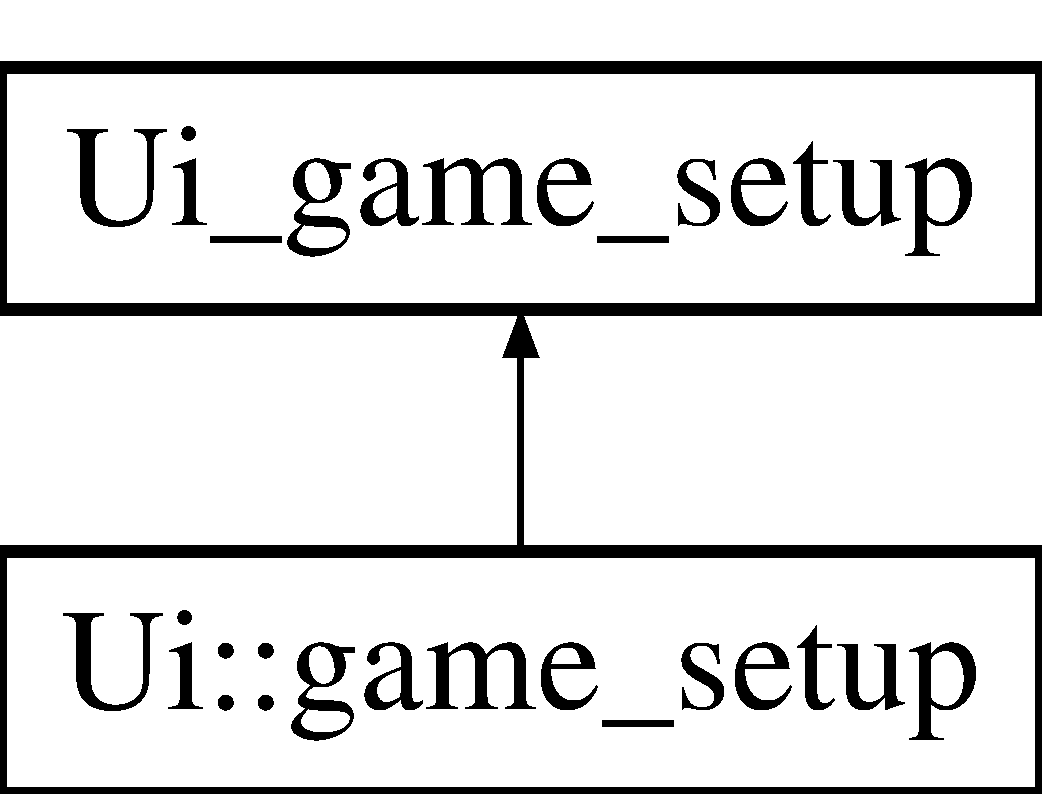
\includegraphics[height=2.000000cm]{classUi_1_1game__setup}
\end{center}
\end{figure}
\subsection*{Additional Inherited Members}


The documentation for this class was generated from the following file\-:\begin{DoxyCompactItemize}
\item 
gui/build-\/client\-\_\-bludiste-\/\-Desktop-\/\-Debug/\hyperlink{ui__game__setup_8h}{ui\-\_\-game\-\_\-setup.\-h}\end{DoxyCompactItemize}

\hypertarget{classgame__setup}{\section{game\-\_\-setup Class Reference}
\label{classgame__setup}\index{game\-\_\-setup@{game\-\_\-setup}}
}


{\ttfamily \#include $<$game\-\_\-setup.\-h$>$}

Inheritance diagram for game\-\_\-setup\-:\begin{figure}[H]
\begin{center}
\leavevmode
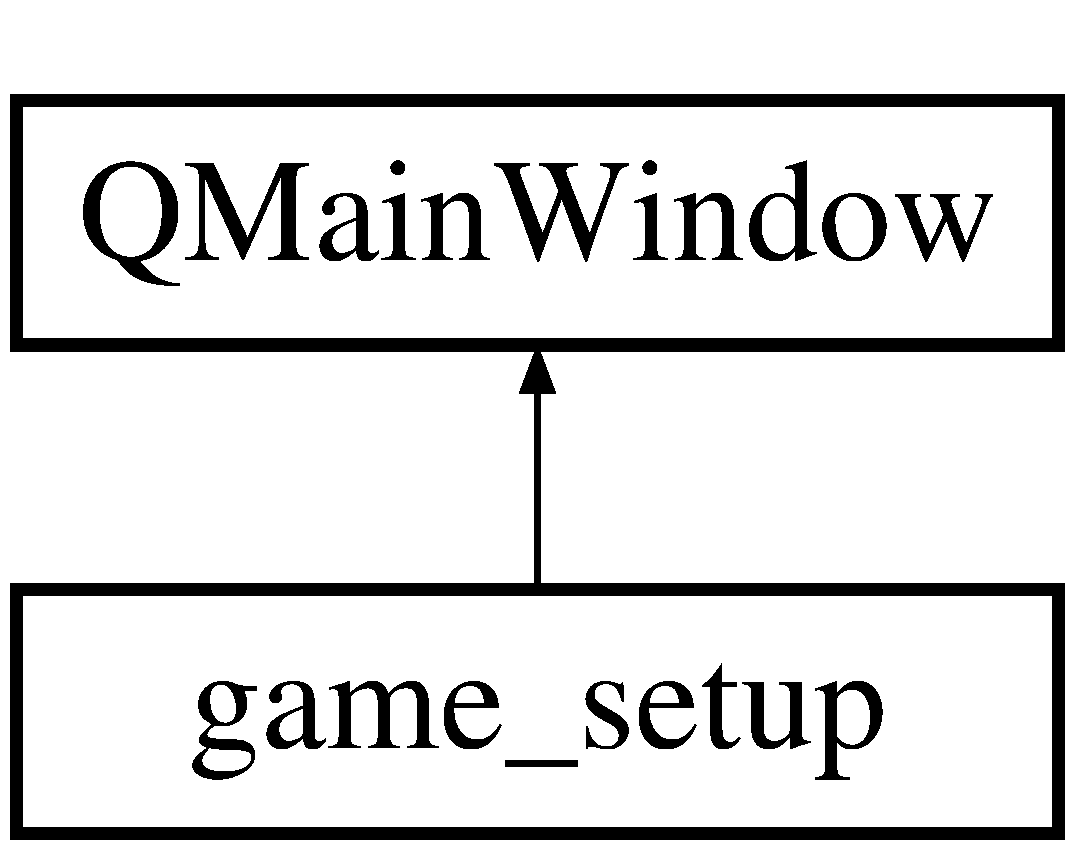
\includegraphics[height=2.000000cm]{classgame__setup}
\end{center}
\end{figure}
\subsection*{Public Member Functions}
\begin{DoxyCompactItemize}
\item 
\hyperlink{classgame__setup_a61492ef3b55322be81a48f6221f527fc}{game\-\_\-setup} (Q\-Widget $\ast$parent=0)
\item 
\hyperlink{classgame__setup_a56511d975fd81988a48b97474eb0b83d}{$\sim$game\-\_\-setup} ()
\item 
void \hyperlink{classgame__setup_ad64efad58a39368041cf58fe401f0e6e}{fullfill\-\_\-client\-\_\-reference} (\hyperlink{classClient}{Client} $\ast$\hyperlink{classgame__setup_adbd0161cc227afe2a8a11c018ee5f139}{client})
\item 
void \hyperlink{classgame__setup_a4bea8d768e958cbc35fa05511ddde8d2}{get\-\_\-maps} ()
\item 
void \hyperlink{classgame__setup_af46808237a6e3b32cef7416c1d210e75}{show\-\_\-available\-\_\-games} ()
\end{DoxyCompactItemize}
\subsection*{Private Slots}
\begin{DoxyCompactItemize}
\item 
void \hyperlink{classgame__setup_a8ff53bb08d7eb073a9cf8cd63f3901e1}{on\-\_\-refresh\-\_\-button\-\_\-clicked} ()
\item 
void \hyperlink{classgame__setup_a620ff00085288b53a1b7cb1a81946b41}{on\-\_\-connect\-\_\-game\-\_\-button\-\_\-clicked} ()
\item 
void \hyperlink{classgame__setup_a02df644221f3577c06cdf4179c99b361}{on\-\_\-create\-\_\-game\-\_\-button\-\_\-clicked} ()
\end{DoxyCompactItemize}
\subsection*{Private Member Functions}
\begin{DoxyCompactItemize}
\item 
void \hyperlink{classgame__setup_ab8e203a71abb83f72a58c44507fbaa35}{insert\-\_\-lines} (std\-::string str, Q\-List\-Widget $\ast$list)
\item 
void \hyperlink{classgame__setup_a3c451d7c5327b93bccd5f7bbc5d27176}{create\-\_\-game\-\_\-window} ()
\end{DoxyCompactItemize}
\subsection*{Private Attributes}
\begin{DoxyCompactItemize}
\item 
\hyperlink{classClient}{Client} $\ast$ \hyperlink{classgame__setup_adbd0161cc227afe2a8a11c018ee5f139}{client}
\item 
\hyperlink{classUi_1_1game__setup}{Ui\-::game\-\_\-setup} $\ast$ \hyperlink{classgame__setup_a025d51998d4c93dd935319c017d6dd00}{ui}
\end{DoxyCompactItemize}


\subsection{Detailed Description}
Třída okna pro připojení do existující hry a pro vytvoření nové hry. Vytváří instanci třídy \hyperlink{classgame__window}{game\-\_\-window} pro samotný běh hry. 

\subsection{Constructor \& Destructor Documentation}
\hypertarget{classgame__setup_a61492ef3b55322be81a48f6221f527fc}{\index{game\-\_\-setup@{game\-\_\-setup}!game\-\_\-setup@{game\-\_\-setup}}
\index{game\-\_\-setup@{game\-\_\-setup}!game_setup@{game\-\_\-setup}}
\subsubsection[{game\-\_\-setup}]{\setlength{\rightskip}{0pt plus 5cm}game\-\_\-setup\-::game\-\_\-setup (
\begin{DoxyParamCaption}
\item[{Q\-Widget $\ast$}]{parent = {\ttfamily 0}}
\end{DoxyParamCaption}
)\hspace{0.3cm}{\ttfamily [explicit]}}}\label{classgame__setup_a61492ef3b55322be81a48f6221f527fc}
\hypertarget{classgame__setup_a56511d975fd81988a48b97474eb0b83d}{\index{game\-\_\-setup@{game\-\_\-setup}!$\sim$game\-\_\-setup@{$\sim$game\-\_\-setup}}
\index{$\sim$game\-\_\-setup@{$\sim$game\-\_\-setup}!game_setup@{game\-\_\-setup}}
\subsubsection[{$\sim$game\-\_\-setup}]{\setlength{\rightskip}{0pt plus 5cm}game\-\_\-setup\-::$\sim$game\-\_\-setup (
\begin{DoxyParamCaption}
{}
\end{DoxyParamCaption}
)}}\label{classgame__setup_a56511d975fd81988a48b97474eb0b83d}


\subsection{Member Function Documentation}
\hypertarget{classgame__setup_a3c451d7c5327b93bccd5f7bbc5d27176}{\index{game\-\_\-setup@{game\-\_\-setup}!create\-\_\-game\-\_\-window@{create\-\_\-game\-\_\-window}}
\index{create\-\_\-game\-\_\-window@{create\-\_\-game\-\_\-window}!game_setup@{game\-\_\-setup}}
\subsubsection[{create\-\_\-game\-\_\-window}]{\setlength{\rightskip}{0pt plus 5cm}void game\-\_\-setup\-::create\-\_\-game\-\_\-window (
\begin{DoxyParamCaption}
{}
\end{DoxyParamCaption}
)\hspace{0.3cm}{\ttfamily [private]}}}\label{classgame__setup_a3c451d7c5327b93bccd5f7bbc5d27176}
Vyvolá vytvoření hracího okna a naplnění reference na třídu \hyperlink{classClient}{Client}. \hypertarget{classgame__setup_ad64efad58a39368041cf58fe401f0e6e}{\index{game\-\_\-setup@{game\-\_\-setup}!fullfill\-\_\-client\-\_\-reference@{fullfill\-\_\-client\-\_\-reference}}
\index{fullfill\-\_\-client\-\_\-reference@{fullfill\-\_\-client\-\_\-reference}!game_setup@{game\-\_\-setup}}
\subsubsection[{fullfill\-\_\-client\-\_\-reference}]{\setlength{\rightskip}{0pt plus 5cm}void game\-\_\-setup\-::fullfill\-\_\-client\-\_\-reference (
\begin{DoxyParamCaption}
\item[{{\bf Client} $\ast$}]{client}
\end{DoxyParamCaption}
)}}\label{classgame__setup_ad64efad58a39368041cf58fe401f0e6e}
Naplění reference na třídu \hyperlink{classClient}{Client}, obsahující informace o hráči a metody pro komunikaci se serverem. \hypertarget{classgame__setup_a4bea8d768e958cbc35fa05511ddde8d2}{\index{game\-\_\-setup@{game\-\_\-setup}!get\-\_\-maps@{get\-\_\-maps}}
\index{get\-\_\-maps@{get\-\_\-maps}!game_setup@{game\-\_\-setup}}
\subsubsection[{get\-\_\-maps}]{\setlength{\rightskip}{0pt plus 5cm}void game\-\_\-setup\-::get\-\_\-maps (
\begin{DoxyParamCaption}
{}
\end{DoxyParamCaption}
)}}\label{classgame__setup_a4bea8d768e958cbc35fa05511ddde8d2}
Volání metody show\-\_\-maps() třídy \hyperlink{classClient}{Client}, pro získání map k dispozici od serveru a jejich zobrazení do listu umístěném v okně metodou insert\-\_\-lines.\par
 V případě chyby je vyvolána výjimka a vypsána chyba (nedojde k ukončení programu). \hypertarget{classgame__setup_ab8e203a71abb83f72a58c44507fbaa35}{\index{game\-\_\-setup@{game\-\_\-setup}!insert\-\_\-lines@{insert\-\_\-lines}}
\index{insert\-\_\-lines@{insert\-\_\-lines}!game_setup@{game\-\_\-setup}}
\subsubsection[{insert\-\_\-lines}]{\setlength{\rightskip}{0pt plus 5cm}void game\-\_\-setup\-::insert\-\_\-lines (
\begin{DoxyParamCaption}
\item[{std\-::string}]{str, }
\item[{Q\-List\-Widget $\ast$}]{list}
\end{DoxyParamCaption}
)\hspace{0.3cm}{\ttfamily [private]}}}\label{classgame__setup_ab8e203a71abb83f72a58c44507fbaa35}
Naparsuje textový řetězec str a zobrazí jednotlivé položky do komponenty instance třídy Q\-List\-Widget. 
\begin{DoxyParams}{Parameters}
{\em str} & Textový řetězec obsahující informace oddělené novým řádkem. \\
\hline
{\em list} & Odkaz na instanci třídy Q\-List\-Widget jenž umožňuje výběr konkrétní položky. \\
\hline
\end{DoxyParams}
\hypertarget{classgame__setup_a620ff00085288b53a1b7cb1a81946b41}{\index{game\-\_\-setup@{game\-\_\-setup}!on\-\_\-connect\-\_\-game\-\_\-button\-\_\-clicked@{on\-\_\-connect\-\_\-game\-\_\-button\-\_\-clicked}}
\index{on\-\_\-connect\-\_\-game\-\_\-button\-\_\-clicked@{on\-\_\-connect\-\_\-game\-\_\-button\-\_\-clicked}!game_setup@{game\-\_\-setup}}
\subsubsection[{on\-\_\-connect\-\_\-game\-\_\-button\-\_\-clicked}]{\setlength{\rightskip}{0pt plus 5cm}void game\-\_\-setup\-::on\-\_\-connect\-\_\-game\-\_\-button\-\_\-clicked (
\begin{DoxyParamCaption}
{}
\end{DoxyParamCaption}
)\hspace{0.3cm}{\ttfamily [private]}, {\ttfamily [slot]}}}\label{classgame__setup_a620ff00085288b53a1b7cb1a81946b41}
Slot reagující na signál vyvolaný kliknutím na tlačítko pro připojení ke hře. \par
 Dojde k odeslání vybrané hry serveru s žádostí o připojení se ke hře. V případě neúspěchu je vypsáno chybové hlášení a dojde k vyvolání výjimky. (Běh programu se neukončí).\par
 V případě úspěchu se vytvoří hrací okno. \hypertarget{classgame__setup_a02df644221f3577c06cdf4179c99b361}{\index{game\-\_\-setup@{game\-\_\-setup}!on\-\_\-create\-\_\-game\-\_\-button\-\_\-clicked@{on\-\_\-create\-\_\-game\-\_\-button\-\_\-clicked}}
\index{on\-\_\-create\-\_\-game\-\_\-button\-\_\-clicked@{on\-\_\-create\-\_\-game\-\_\-button\-\_\-clicked}!game_setup@{game\-\_\-setup}}
\subsubsection[{on\-\_\-create\-\_\-game\-\_\-button\-\_\-clicked}]{\setlength{\rightskip}{0pt plus 5cm}void game\-\_\-setup\-::on\-\_\-create\-\_\-game\-\_\-button\-\_\-clicked (
\begin{DoxyParamCaption}
{}
\end{DoxyParamCaption}
)\hspace{0.3cm}{\ttfamily [private]}, {\ttfamily [slot]}}}\label{classgame__setup_a02df644221f3577c06cdf4179c99b361}
Slot reagující na signál vyvolaný kliknutím na tlačítko pro vytvoření hry. \par
 Dojde k odeslání vybrané mapy serveru s žádostí o vytvoření hry. V případě neúspěchu je vypsáno chybové hlášení a dojde k vyvolání výjimky. (Běh programu se neukončí). \par
 V případě úspěchu se vytvoří hrací okno. \hypertarget{classgame__setup_a8ff53bb08d7eb073a9cf8cd63f3901e1}{\index{game\-\_\-setup@{game\-\_\-setup}!on\-\_\-refresh\-\_\-button\-\_\-clicked@{on\-\_\-refresh\-\_\-button\-\_\-clicked}}
\index{on\-\_\-refresh\-\_\-button\-\_\-clicked@{on\-\_\-refresh\-\_\-button\-\_\-clicked}!game_setup@{game\-\_\-setup}}
\subsubsection[{on\-\_\-refresh\-\_\-button\-\_\-clicked}]{\setlength{\rightskip}{0pt plus 5cm}void game\-\_\-setup\-::on\-\_\-refresh\-\_\-button\-\_\-clicked (
\begin{DoxyParamCaption}
{}
\end{DoxyParamCaption}
)\hspace{0.3cm}{\ttfamily [private]}, {\ttfamily [slot]}}}\label{classgame__setup_a8ff53bb08d7eb073a9cf8cd63f3901e1}
Slot reagující na signál vyvolaný kliknutím na tlačítko aktualizovat. Vyvolá metodu get\-\_\-games a dojde k zobrazení aktuálně rozehraných her. \hypertarget{classgame__setup_af46808237a6e3b32cef7416c1d210e75}{\index{game\-\_\-setup@{game\-\_\-setup}!show\-\_\-available\-\_\-games@{show\-\_\-available\-\_\-games}}
\index{show\-\_\-available\-\_\-games@{show\-\_\-available\-\_\-games}!game_setup@{game\-\_\-setup}}
\subsubsection[{show\-\_\-available\-\_\-games}]{\setlength{\rightskip}{0pt plus 5cm}void game\-\_\-setup\-::show\-\_\-available\-\_\-games (
\begin{DoxyParamCaption}
{}
\end{DoxyParamCaption}
)}}\label{classgame__setup_af46808237a6e3b32cef7416c1d210e75}
Zavolá funkci get\-\_\-games() třídy \hyperlink{classClient}{Client} a zobrazí všechny rozehrané hry v okně. V případě chyby je vyvolána výjimka a vypsána chyba (nedojde k ukončení programu). 

\subsection{Member Data Documentation}
\hypertarget{classgame__setup_adbd0161cc227afe2a8a11c018ee5f139}{\index{game\-\_\-setup@{game\-\_\-setup}!client@{client}}
\index{client@{client}!game_setup@{game\-\_\-setup}}
\subsubsection[{client}]{\setlength{\rightskip}{0pt plus 5cm}{\bf Client}$\ast$ game\-\_\-setup\-::client\hspace{0.3cm}{\ttfamily [private]}}}\label{classgame__setup_adbd0161cc227afe2a8a11c018ee5f139}
\hypertarget{classgame__setup_a025d51998d4c93dd935319c017d6dd00}{\index{game\-\_\-setup@{game\-\_\-setup}!ui@{ui}}
\index{ui@{ui}!game_setup@{game\-\_\-setup}}
\subsubsection[{ui}]{\setlength{\rightskip}{0pt plus 5cm}{\bf Ui\-::game\-\_\-setup}$\ast$ game\-\_\-setup\-::ui\hspace{0.3cm}{\ttfamily [private]}}}\label{classgame__setup_a025d51998d4c93dd935319c017d6dd00}


The documentation for this class was generated from the following files\-:\begin{DoxyCompactItemize}
\item 
gui/client\-\_\-bludiste/\hyperlink{game__setup_8h}{game\-\_\-setup.\-h}\item 
gui/client\-\_\-bludiste/\hyperlink{game__setup_8cpp}{game\-\_\-setup.\-cpp}\end{DoxyCompactItemize}

\hypertarget{classUi_1_1game__window}{\section{Ui\-:\-:game\-\_\-window Class Reference}
\label{classUi_1_1game__window}\index{Ui\-::game\-\_\-window@{Ui\-::game\-\_\-window}}
}


{\ttfamily \#include $<$ui\-\_\-game\-\_\-window.\-h$>$}

Inheritance diagram for Ui\-:\-:game\-\_\-window\-:\begin{figure}[H]
\begin{center}
\leavevmode
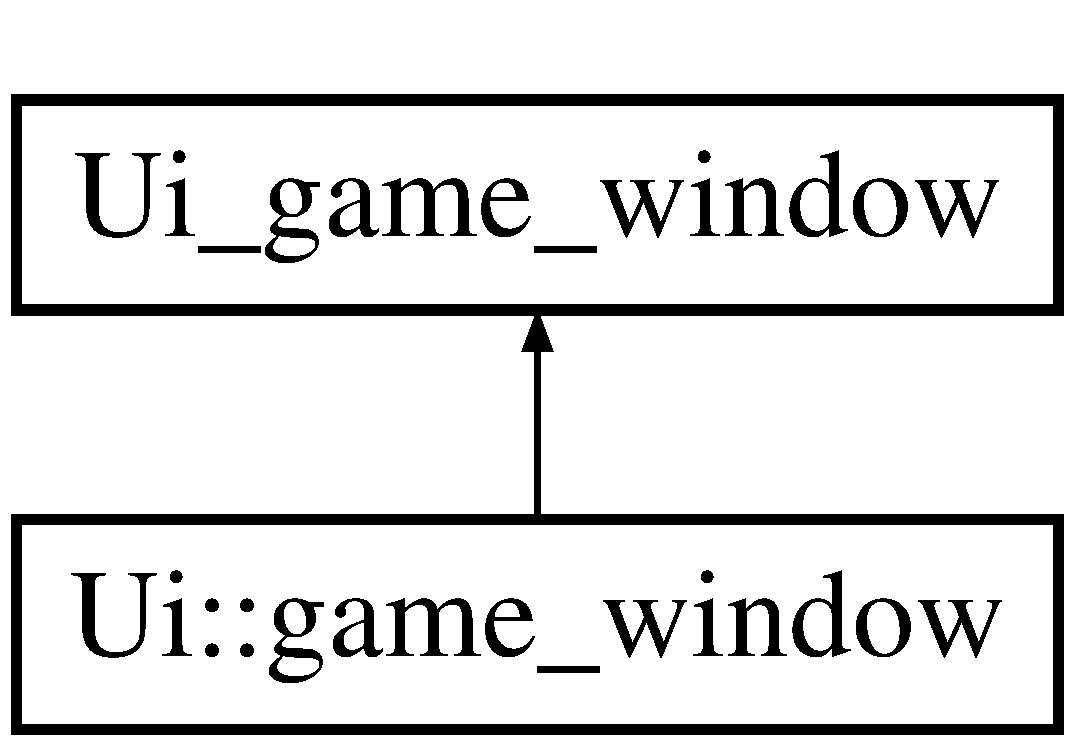
\includegraphics[height=2.000000cm]{classUi_1_1game__window}
\end{center}
\end{figure}
\subsection*{Additional Inherited Members}


The documentation for this class was generated from the following file\-:\begin{DoxyCompactItemize}
\item 
gui/build-\/client\-\_\-bludiste-\/\-Desktop-\/\-Debug/\hyperlink{ui__game__window_8h}{ui\-\_\-game\-\_\-window.\-h}\end{DoxyCompactItemize}

\hypertarget{classgame__window}{\section{game\-\_\-window Class Reference}
\label{classgame__window}\index{game\-\_\-window@{game\-\_\-window}}
}


{\ttfamily \#include $<$game\-\_\-window.\-h$>$}

Inheritance diagram for game\-\_\-window\-:\begin{figure}[H]
\begin{center}
\leavevmode
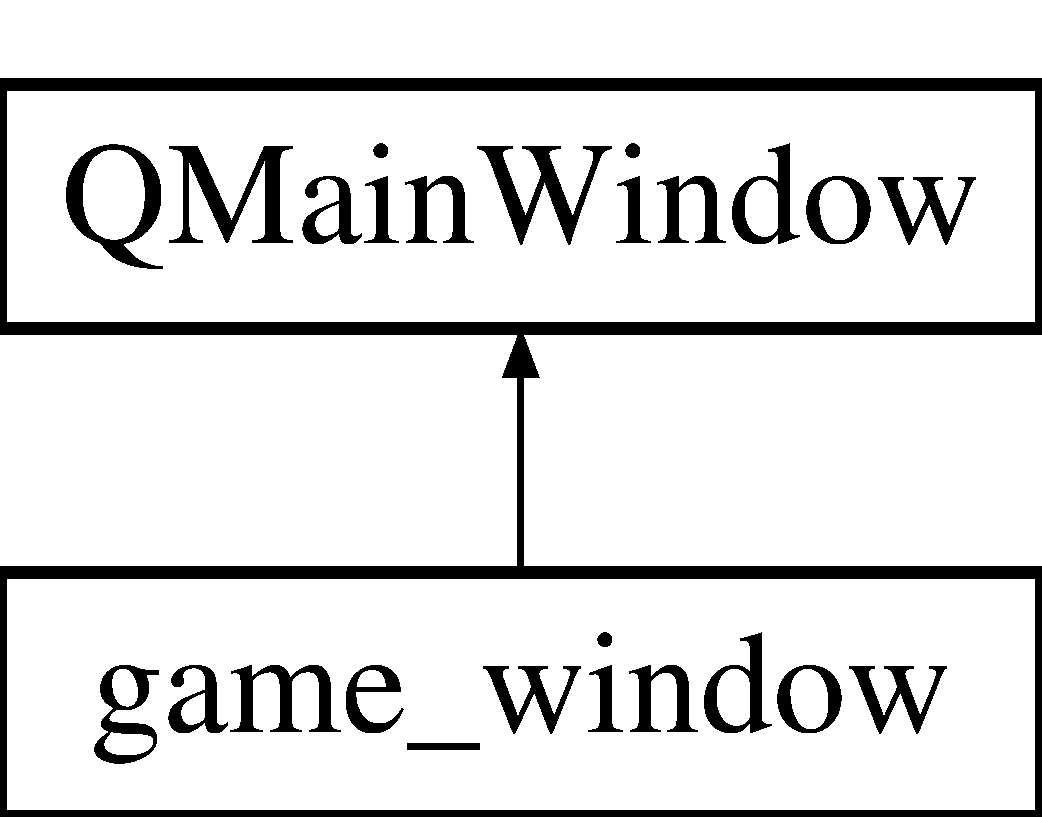
\includegraphics[height=2.000000cm]{classgame__window}
\end{center}
\end{figure}
\subsection*{Public Member Functions}
\begin{DoxyCompactItemize}
\item 
\hyperlink{classgame__window_ab5c211ed2b0c1f224bab4a38bd1b6949}{game\-\_\-window} (Q\-Widget $\ast$parent=0)
\item 
\hyperlink{classgame__window_a9766be5a2cd86e94a14618f5a2817aad}{$\sim$game\-\_\-window} ()
\item 
void \hyperlink{classgame__window_a5f515ec0cce41575760ed2e11dd43192}{fullfill\-\_\-client\-\_\-reference} (\hyperlink{classClient}{Client} $\ast$\hyperlink{classgame__window_a5d8487b5833826ceb57f78dd4df08a36}{client})
\item 
void \hyperlink{classgame__window_a2b6b63f1366a2ae287097ba571230752}{create\-\_\-game\-\_\-field} ()
\item 
void \hyperlink{classgame__window_a9ac4ef3fad106217a101ed1b0324636f}{print\-\_\-map} ()
\end{DoxyCompactItemize}
\subsection*{Private Slots}
\begin{DoxyCompactItemize}
\item 
void \hyperlink{classgame__window_a81dcbe35cf90a64db2728139a800a782}{on\-\_\-send\-\_\-command\-\_\-button\-\_\-clicked} ()
\end{DoxyCompactItemize}
\subsection*{Private Attributes}
\begin{DoxyCompactItemize}
\item 
\hyperlink{classClient}{Client} $\ast$ \hyperlink{classgame__window_a5d8487b5833826ceb57f78dd4df08a36}{client}
\item 
\hyperlink{classUi_1_1game__window}{Ui\-::game\-\_\-window} $\ast$ \hyperlink{classgame__window_ae3ab3ecb88eadc7f9929c774a9c338bb}{ui}
\end{DoxyCompactItemize}


\subsection{Detailed Description}
Třída dědící od třídy Q\-Main\-Window. Obsahuje odkaz na třídu \hyperlink{classClient}{Client}, obsahující informace o hráři a implementaci metod pro komunikaci se serverem. 

\subsection{Constructor \& Destructor Documentation}
\hypertarget{classgame__window_ab5c211ed2b0c1f224bab4a38bd1b6949}{\index{game\-\_\-window@{game\-\_\-window}!game\-\_\-window@{game\-\_\-window}}
\index{game\-\_\-window@{game\-\_\-window}!game_window@{game\-\_\-window}}
\subsubsection[{game\-\_\-window}]{\setlength{\rightskip}{0pt plus 5cm}game\-\_\-window\-::game\-\_\-window (
\begin{DoxyParamCaption}
\item[{Q\-Widget $\ast$}]{parent = {\ttfamily 0}}
\end{DoxyParamCaption}
)\hspace{0.3cm}{\ttfamily [explicit]}}}\label{classgame__window_ab5c211ed2b0c1f224bab4a38bd1b6949}
\hypertarget{classgame__window_a9766be5a2cd86e94a14618f5a2817aad}{\index{game\-\_\-window@{game\-\_\-window}!$\sim$game\-\_\-window@{$\sim$game\-\_\-window}}
\index{$\sim$game\-\_\-window@{$\sim$game\-\_\-window}!game_window@{game\-\_\-window}}
\subsubsection[{$\sim$game\-\_\-window}]{\setlength{\rightskip}{0pt plus 5cm}game\-\_\-window\-::$\sim$game\-\_\-window (
\begin{DoxyParamCaption}
{}
\end{DoxyParamCaption}
)}}\label{classgame__window_a9766be5a2cd86e94a14618f5a2817aad}


\subsection{Member Function Documentation}
\hypertarget{classgame__window_a2b6b63f1366a2ae287097ba571230752}{\index{game\-\_\-window@{game\-\_\-window}!create\-\_\-game\-\_\-field@{create\-\_\-game\-\_\-field}}
\index{create\-\_\-game\-\_\-field@{create\-\_\-game\-\_\-field}!game_window@{game\-\_\-window}}
\subsubsection[{create\-\_\-game\-\_\-field}]{\setlength{\rightskip}{0pt plus 5cm}void game\-\_\-window\-::create\-\_\-game\-\_\-field (
\begin{DoxyParamCaption}
{}
\end{DoxyParamCaption}
)}}\label{classgame__window_a2b6b63f1366a2ae287097ba571230752}
Funkce pro vytvoření hracího okna. Dynamicky nastavuje velikost okna podle rozměrů hrací plochy. Dynamicky umisťuje jednotlivé komponenty podle rozměrů okna. alokuje hrací plochu a propojuje ji s mřížkou umístěnou v grafickém rozhraní. \hypertarget{classgame__window_a5f515ec0cce41575760ed2e11dd43192}{\index{game\-\_\-window@{game\-\_\-window}!fullfill\-\_\-client\-\_\-reference@{fullfill\-\_\-client\-\_\-reference}}
\index{fullfill\-\_\-client\-\_\-reference@{fullfill\-\_\-client\-\_\-reference}!game_window@{game\-\_\-window}}
\subsubsection[{fullfill\-\_\-client\-\_\-reference}]{\setlength{\rightskip}{0pt plus 5cm}void game\-\_\-window\-::fullfill\-\_\-client\-\_\-reference (
\begin{DoxyParamCaption}
\item[{{\bf Client} $\ast$}]{client}
\end{DoxyParamCaption}
)}}\label{classgame__window_a5f515ec0cce41575760ed2e11dd43192}
Naplní odkaz na třídu \hyperlink{classClient}{Client} obsahující funkce pro komunikaci se serverem a informace o hráči. \hypertarget{classgame__window_a81dcbe35cf90a64db2728139a800a782}{\index{game\-\_\-window@{game\-\_\-window}!on\-\_\-send\-\_\-command\-\_\-button\-\_\-clicked@{on\-\_\-send\-\_\-command\-\_\-button\-\_\-clicked}}
\index{on\-\_\-send\-\_\-command\-\_\-button\-\_\-clicked@{on\-\_\-send\-\_\-command\-\_\-button\-\_\-clicked}!game_window@{game\-\_\-window}}
\subsubsection[{on\-\_\-send\-\_\-command\-\_\-button\-\_\-clicked}]{\setlength{\rightskip}{0pt plus 5cm}void game\-\_\-window\-::on\-\_\-send\-\_\-command\-\_\-button\-\_\-clicked (
\begin{DoxyParamCaption}
{}
\end{DoxyParamCaption}
)\hspace{0.3cm}{\ttfamily [private]}, {\ttfamily [slot]}}}\label{classgame__window_a81dcbe35cf90a64db2728139a800a782}
Slot reagující na signál vyvolaný stisknutím tlačítka potvrzení příkazu. V případě chyby (neexistujícího příkazu) dojde k vyvolání výjimky a vypsání chybové hlášky (bez ukončení programu). \hypertarget{classgame__window_a9ac4ef3fad106217a101ed1b0324636f}{\index{game\-\_\-window@{game\-\_\-window}!print\-\_\-map@{print\-\_\-map}}
\index{print\-\_\-map@{print\-\_\-map}!game_window@{game\-\_\-window}}
\subsubsection[{print\-\_\-map}]{\setlength{\rightskip}{0pt plus 5cm}void game\-\_\-window\-::print\-\_\-map (
\begin{DoxyParamCaption}
{}
\end{DoxyParamCaption}
)}}\label{classgame__window_a9ac4ef3fad106217a101ed1b0324636f}


\subsection{Member Data Documentation}
\hypertarget{classgame__window_a5d8487b5833826ceb57f78dd4df08a36}{\index{game\-\_\-window@{game\-\_\-window}!client@{client}}
\index{client@{client}!game_window@{game\-\_\-window}}
\subsubsection[{client}]{\setlength{\rightskip}{0pt plus 5cm}{\bf Client}$\ast$ game\-\_\-window\-::client\hspace{0.3cm}{\ttfamily [private]}}}\label{classgame__window_a5d8487b5833826ceb57f78dd4df08a36}
\hypertarget{classgame__window_ae3ab3ecb88eadc7f9929c774a9c338bb}{\index{game\-\_\-window@{game\-\_\-window}!ui@{ui}}
\index{ui@{ui}!game_window@{game\-\_\-window}}
\subsubsection[{ui}]{\setlength{\rightskip}{0pt plus 5cm}{\bf Ui\-::game\-\_\-window}$\ast$ game\-\_\-window\-::ui\hspace{0.3cm}{\ttfamily [private]}}}\label{classgame__window_ae3ab3ecb88eadc7f9929c774a9c338bb}


The documentation for this class was generated from the following files\-:\begin{DoxyCompactItemize}
\item 
gui/client\-\_\-bludiste/\hyperlink{game__window_8h}{game\-\_\-window.\-h}\item 
gui/client\-\_\-bludiste/\hyperlink{game__window_8cpp}{game\-\_\-window.\-cpp}\end{DoxyCompactItemize}

\input{structqt__meta__stringdata__game__setup__t}
\input{structqt__meta__stringdata__game__window__t}
\input{structqt__meta__stringdata__server__connection__window__t}
\hypertarget{classserver__connection__window}{\section{server\-\_\-connection\-\_\-window Class Reference}
\label{classserver__connection__window}\index{server\-\_\-connection\-\_\-window@{server\-\_\-connection\-\_\-window}}
}


{\ttfamily \#include $<$server\-\_\-connection\-\_\-window.\-h$>$}

Inheritance diagram for server\-\_\-connection\-\_\-window\-:\begin{figure}[H]
\begin{center}
\leavevmode
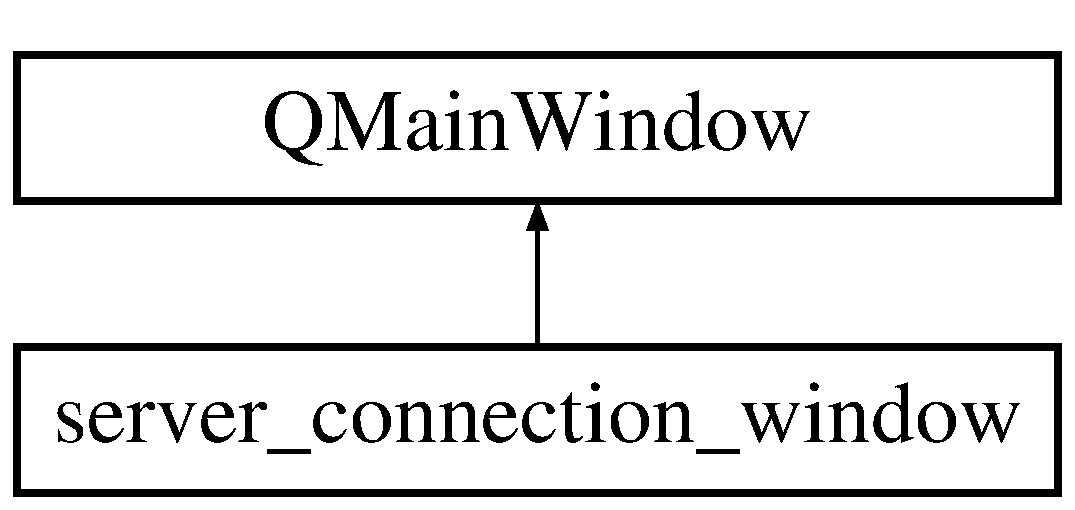
\includegraphics[height=2.000000cm]{classserver__connection__window}
\end{center}
\end{figure}
\subsection*{Public Member Functions}
\begin{DoxyCompactItemize}
\item 
\hyperlink{classserver__connection__window_a5c4228ae40722c21d5aaf33044d65e8c}{server\-\_\-connection\-\_\-window} (Q\-Widget $\ast$parent=0)
\item 
\hyperlink{classserver__connection__window_a4cb59e06328d101c22a5a0d1a0285faf}{$\sim$server\-\_\-connection\-\_\-window} ()
\item 
void \hyperlink{classserver__connection__window_a0e494399c11e10e00688bcbca8dc7053}{fullfill\-\_\-client\-\_\-reference} (\hyperlink{classClient}{Client} $\ast$\hyperlink{classserver__connection__window_aedf2c1c7bec9b66101617dfd75cc61cc}{client})
\end{DoxyCompactItemize}
\subsection*{Private Slots}
\begin{DoxyCompactItemize}
\item 
void \hyperlink{classserver__connection__window_afed61024df5469b7a947f53b1fa1c1da}{on\-\_\-server\-\_\-connect\-\_\-button\-\_\-clicked} ()
\end{DoxyCompactItemize}
\subsection*{Private Attributes}
\begin{DoxyCompactItemize}
\item 
\hyperlink{classClient}{Client} $\ast$ \hyperlink{classserver__connection__window_aedf2c1c7bec9b66101617dfd75cc61cc}{client}
\item 
\hyperlink{classUi_1_1server__connection__window}{Ui\-::server\-\_\-connection\-\_\-window} $\ast$ \hyperlink{classserver__connection__window_aafa54aec3e044c301c95915b68aae75f}{ui}
\end{DoxyCompactItemize}


\subsection{Detailed Description}
Obsahuje zobrazitelné okno, ve kterém je vyžadována adresa serveru. Dochází ke kontrole zda server existuje (pomocí funkcí třídy \hyperlink{classClient}{Client}) a v pozitivním případě dojde k připojení k serveru. V případě že server neexistuje dojde k vyvolání vyjímky, okno vypíše chybové hlášení , a hráč má možnost pokusit se připojit znovu (vyvoláním výjimky nedojde k vypnutí programu). \par
\par
 Grafické rozhraní okna pro připojení bylo vytvořeno pomocí Q\-T Creatoru a je uloženo v \hyperlink{classserver__connection__window_aafa54aec3e044c301c95915b68aae75f}{server\-\_\-connection\-\_\-window.\-ui}. 

\subsection{Constructor \& Destructor Documentation}
\hypertarget{classserver__connection__window_a5c4228ae40722c21d5aaf33044d65e8c}{\index{server\-\_\-connection\-\_\-window@{server\-\_\-connection\-\_\-window}!server\-\_\-connection\-\_\-window@{server\-\_\-connection\-\_\-window}}
\index{server\-\_\-connection\-\_\-window@{server\-\_\-connection\-\_\-window}!server_connection_window@{server\-\_\-connection\-\_\-window}}
\subsubsection[{server\-\_\-connection\-\_\-window}]{\setlength{\rightskip}{0pt plus 5cm}server\-\_\-connection\-\_\-window\-::server\-\_\-connection\-\_\-window (
\begin{DoxyParamCaption}
\item[{Q\-Widget $\ast$}]{parent = {\ttfamily 0}}
\end{DoxyParamCaption}
)\hspace{0.3cm}{\ttfamily [explicit]}}}\label{classserver__connection__window_a5c4228ae40722c21d5aaf33044d65e8c}
\hypertarget{classserver__connection__window_a4cb59e06328d101c22a5a0d1a0285faf}{\index{server\-\_\-connection\-\_\-window@{server\-\_\-connection\-\_\-window}!$\sim$server\-\_\-connection\-\_\-window@{$\sim$server\-\_\-connection\-\_\-window}}
\index{$\sim$server\-\_\-connection\-\_\-window@{$\sim$server\-\_\-connection\-\_\-window}!server_connection_window@{server\-\_\-connection\-\_\-window}}
\subsubsection[{$\sim$server\-\_\-connection\-\_\-window}]{\setlength{\rightskip}{0pt plus 5cm}server\-\_\-connection\-\_\-window\-::$\sim$server\-\_\-connection\-\_\-window (
\begin{DoxyParamCaption}
{}
\end{DoxyParamCaption}
)}}\label{classserver__connection__window_a4cb59e06328d101c22a5a0d1a0285faf}


\subsection{Member Function Documentation}
\hypertarget{classserver__connection__window_a0e494399c11e10e00688bcbca8dc7053}{\index{server\-\_\-connection\-\_\-window@{server\-\_\-connection\-\_\-window}!fullfill\-\_\-client\-\_\-reference@{fullfill\-\_\-client\-\_\-reference}}
\index{fullfill\-\_\-client\-\_\-reference@{fullfill\-\_\-client\-\_\-reference}!server_connection_window@{server\-\_\-connection\-\_\-window}}
\subsubsection[{fullfill\-\_\-client\-\_\-reference}]{\setlength{\rightskip}{0pt plus 5cm}void server\-\_\-connection\-\_\-window\-::fullfill\-\_\-client\-\_\-reference (
\begin{DoxyParamCaption}
\item[{{\bf Client} $\ast$}]{client}
\end{DoxyParamCaption}
)}}\label{classserver__connection__window_a0e494399c11e10e00688bcbca8dc7053}
Provádí navázání reference na třídu \hyperlink{classClient}{Client}, která obsahuje veškeré informace o hráči a funkce pro práci s komunikací se serverem. \hypertarget{classserver__connection__window_afed61024df5469b7a947f53b1fa1c1da}{\index{server\-\_\-connection\-\_\-window@{server\-\_\-connection\-\_\-window}!on\-\_\-server\-\_\-connect\-\_\-button\-\_\-clicked@{on\-\_\-server\-\_\-connect\-\_\-button\-\_\-clicked}}
\index{on\-\_\-server\-\_\-connect\-\_\-button\-\_\-clicked@{on\-\_\-server\-\_\-connect\-\_\-button\-\_\-clicked}!server_connection_window@{server\-\_\-connection\-\_\-window}}
\subsubsection[{on\-\_\-server\-\_\-connect\-\_\-button\-\_\-clicked}]{\setlength{\rightskip}{0pt plus 5cm}void server\-\_\-connection\-\_\-window\-::on\-\_\-server\-\_\-connect\-\_\-button\-\_\-clicked (
\begin{DoxyParamCaption}
{}
\end{DoxyParamCaption}
)\hspace{0.3cm}{\ttfamily [private]}, {\ttfamily [slot]}}}\label{classserver__connection__window_afed61024df5469b7a947f53b1fa1c1da}
Funkce reagující na signál vyvolaný kliknutím na tlačítko připojit. \par
 Dojde k pokusu o připojení k serveru v okně pro zadání adresy serveru. Pokud se k serveru nepodaří připojit, vygeneruje se výjimka která se projeví vypsáním chybové hlášky. Program umožňuje nové zadání adresy serveru (vyvoláním výjimky nedojde k ukončení programu). 

\subsection{Member Data Documentation}
\hypertarget{classserver__connection__window_aedf2c1c7bec9b66101617dfd75cc61cc}{\index{server\-\_\-connection\-\_\-window@{server\-\_\-connection\-\_\-window}!client@{client}}
\index{client@{client}!server_connection_window@{server\-\_\-connection\-\_\-window}}
\subsubsection[{client}]{\setlength{\rightskip}{0pt plus 5cm}{\bf Client}$\ast$ server\-\_\-connection\-\_\-window\-::client\hspace{0.3cm}{\ttfamily [private]}}}\label{classserver__connection__window_aedf2c1c7bec9b66101617dfd75cc61cc}
\hypertarget{classserver__connection__window_aafa54aec3e044c301c95915b68aae75f}{\index{server\-\_\-connection\-\_\-window@{server\-\_\-connection\-\_\-window}!ui@{ui}}
\index{ui@{ui}!server_connection_window@{server\-\_\-connection\-\_\-window}}
\subsubsection[{ui}]{\setlength{\rightskip}{0pt plus 5cm}{\bf Ui\-::server\-\_\-connection\-\_\-window}$\ast$ server\-\_\-connection\-\_\-window\-::ui\hspace{0.3cm}{\ttfamily [private]}}}\label{classserver__connection__window_aafa54aec3e044c301c95915b68aae75f}


The documentation for this class was generated from the following files\-:\begin{DoxyCompactItemize}
\item 
gui/client\-\_\-bludiste/\hyperlink{server__connection__window_8h}{server\-\_\-connection\-\_\-window.\-h}\item 
gui/client\-\_\-bludiste/\hyperlink{server__connection__window_8cpp}{server\-\_\-connection\-\_\-window.\-cpp}\end{DoxyCompactItemize}

\hypertarget{classUi_1_1server__connection__window}{\section{Ui\-:\-:server\-\_\-connection\-\_\-window Class Reference}
\label{classUi_1_1server__connection__window}\index{Ui\-::server\-\_\-connection\-\_\-window@{Ui\-::server\-\_\-connection\-\_\-window}}
}


{\ttfamily \#include $<$ui\-\_\-server\-\_\-connection\-\_\-window.\-h$>$}

Inheritance diagram for Ui\-:\-:server\-\_\-connection\-\_\-window\-:\begin{figure}[H]
\begin{center}
\leavevmode
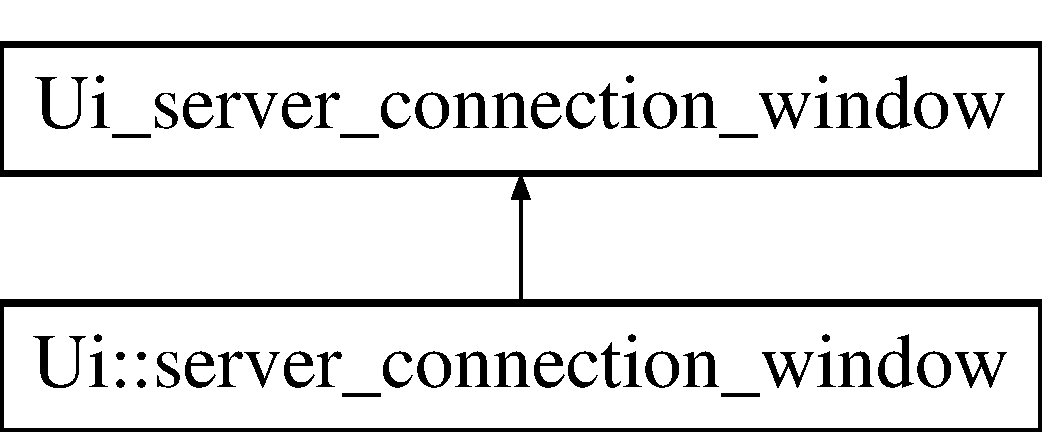
\includegraphics[height=2.000000cm]{classUi_1_1server__connection__window}
\end{center}
\end{figure}
\subsection*{Additional Inherited Members}


The documentation for this class was generated from the following file\-:\begin{DoxyCompactItemize}
\item 
gui/build-\/client\-\_\-bludiste-\/\-Desktop-\/\-Debug/\hyperlink{ui__server__connection__window_8h}{ui\-\_\-server\-\_\-connection\-\_\-window.\-h}\end{DoxyCompactItemize}

\hypertarget{classUi_1_1Setup__menu}{\section{Ui\-:\-:Setup\-\_\-menu Class Reference}
\label{classUi_1_1Setup__menu}\index{Ui\-::\-Setup\-\_\-menu@{Ui\-::\-Setup\-\_\-menu}}
}


{\ttfamily \#include $<$ui\-\_\-setup\-\_\-menu.\-h$>$}

Inheritance diagram for Ui\-:\-:Setup\-\_\-menu\-:\begin{figure}[H]
\begin{center}
\leavevmode
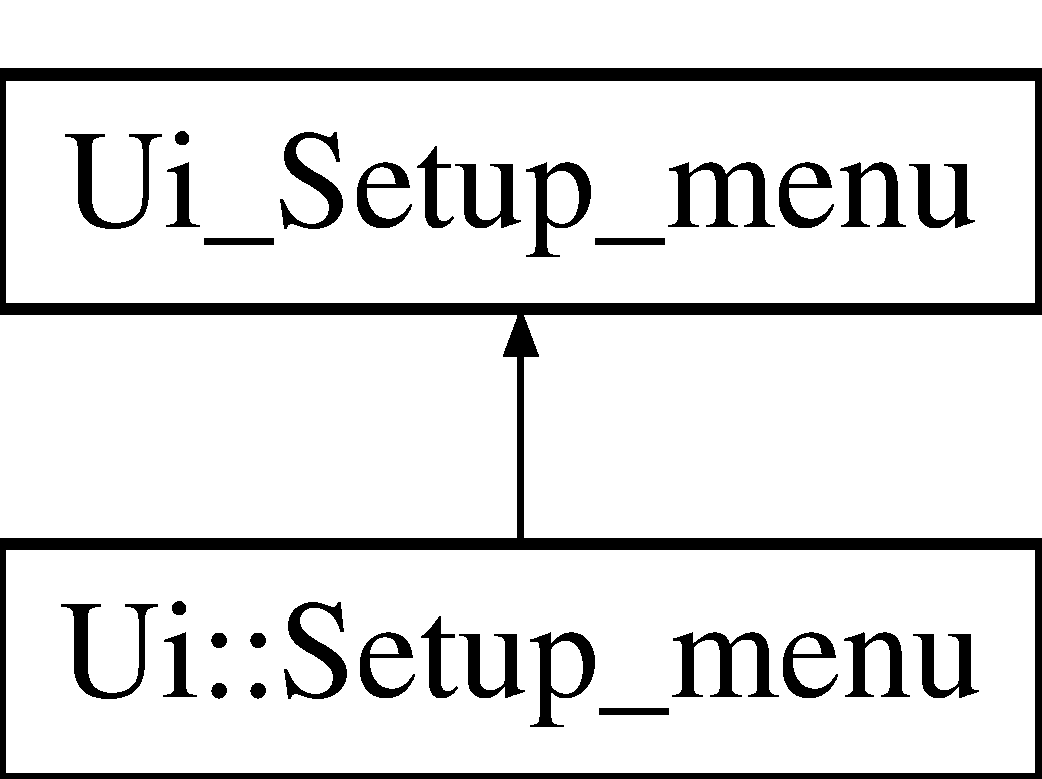
\includegraphics[height=2.000000cm]{classUi_1_1Setup__menu}
\end{center}
\end{figure}
\subsection*{Additional Inherited Members}


The documentation for this class was generated from the following file\-:\begin{DoxyCompactItemize}
\item 
\hyperlink{ui__setup__menu_8h}{ui\-\_\-setup\-\_\-menu.\-h}\end{DoxyCompactItemize}

\hypertarget{classUi__game__setup}{\section{Ui\-\_\-game\-\_\-setup Class Reference}
\label{classUi__game__setup}\index{Ui\-\_\-game\-\_\-setup@{Ui\-\_\-game\-\_\-setup}}
}


{\ttfamily \#include $<$ui\-\_\-game\-\_\-setup.\-h$>$}

Inheritance diagram for Ui\-\_\-game\-\_\-setup\-:\begin{figure}[H]
\begin{center}
\leavevmode
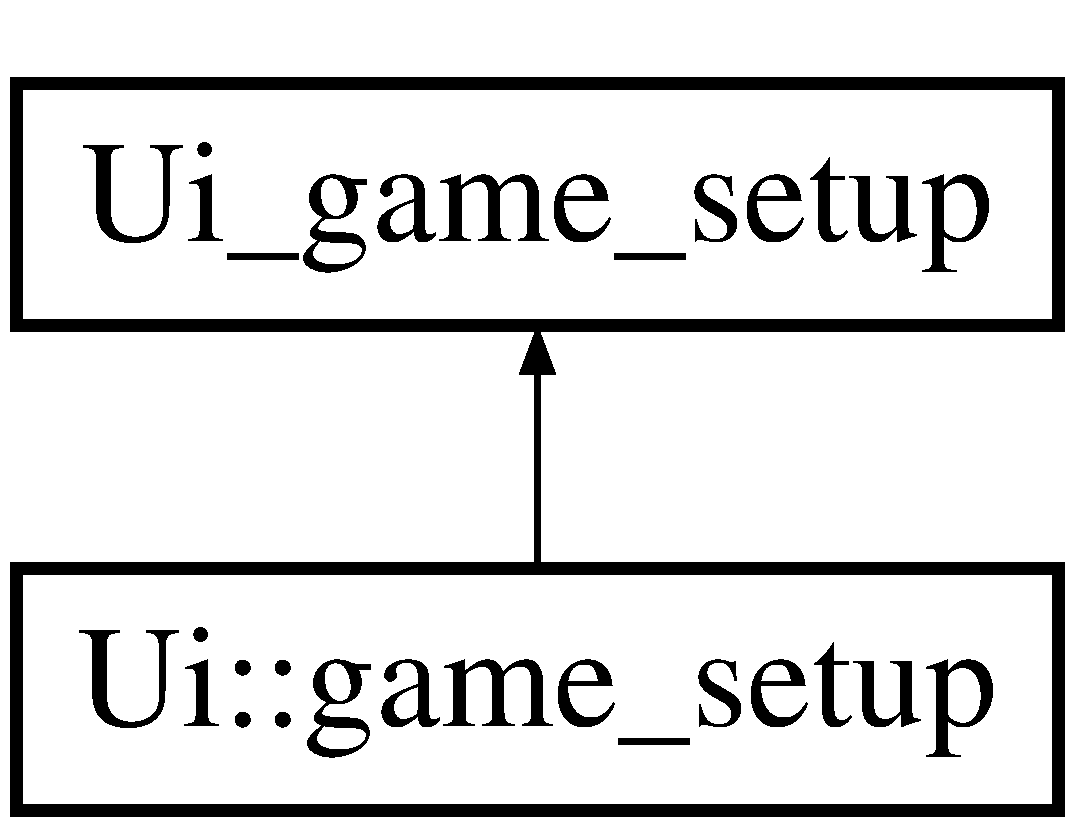
\includegraphics[height=2.000000cm]{classUi__game__setup}
\end{center}
\end{figure}
\subsection*{Public Member Functions}
\begin{DoxyCompactItemize}
\item 
void \hyperlink{classUi__game__setup_a106d59c06db7a08cb512d2491e65f587}{setup\-Ui} (Q\-Main\-Window $\ast$\hyperlink{classgame__setup}{game\-\_\-setup})
\item 
void \hyperlink{classUi__game__setup_a8f65fdf39c952a235cd75ff04d3a0167}{retranslate\-Ui} (Q\-Main\-Window $\ast$\hyperlink{classgame__setup}{game\-\_\-setup})
\end{DoxyCompactItemize}
\subsection*{Public Attributes}
\begin{DoxyCompactItemize}
\item 
Q\-Widget $\ast$ \hyperlink{classUi__game__setup_a4dfcb4d3bf0a2f29f9bc8354c9687dfd}{central\-Widget}
\item 
Q\-Label $\ast$ \hyperlink{classUi__game__setup_af247cb7103f2893112b515a475f88ae1}{label}
\item 
Q\-Push\-Button $\ast$ \hyperlink{classUi__game__setup_a91b386cf441741790b6e05490fda2559}{connect\-\_\-game\-\_\-button}
\item 
Q\-Label $\ast$ \hyperlink{classUi__game__setup_abb56f61c24a4993abeef283af64ab411}{label\-\_\-2}
\item 
Q\-Push\-Button $\ast$ \hyperlink{classUi__game__setup_a272a6d3379864cedacdcb5f39cce438b}{create\-\_\-game\-\_\-button}
\item 
Q\-Push\-Button $\ast$ \hyperlink{classUi__game__setup_a1982cdaf064bb3a8f784254050159973}{refresh\-\_\-button}
\item 
Q\-List\-Widget $\ast$ \hyperlink{classUi__game__setup_a5f16472eaa18f7bd1aa1ce30d5362a1c}{games\-\_\-viewer}
\item 
Q\-List\-Widget $\ast$ \hyperlink{classUi__game__setup_a5a0c74d0c52179ccaa7703770cece094}{maps\-\_\-list}
\item 
Q\-Label $\ast$ \hyperlink{classUi__game__setup_af02f3182e60b85fbd75f65937fe46c91}{when\-\_\-error\-\_\-label}
\item 
Q\-Label $\ast$ \hyperlink{classUi__game__setup_a0d0d4dce33543ffae0b76c7d7e1b9b51}{label\-\_\-3}
\item 
Q\-Double\-Spin\-Box $\ast$ \hyperlink{classUi__game__setup_a40da11a9746d8882462ed1f493c193b2}{timeout\-\_\-edit}
\item 
Q\-Menu\-Bar $\ast$ \hyperlink{classUi__game__setup_a9a7e53627ea76bb9080ec7b26c160a12}{menu\-Bar}
\end{DoxyCompactItemize}


\subsection{Member Function Documentation}
\hypertarget{classUi__game__setup_a8f65fdf39c952a235cd75ff04d3a0167}{\index{Ui\-\_\-game\-\_\-setup@{Ui\-\_\-game\-\_\-setup}!retranslate\-Ui@{retranslate\-Ui}}
\index{retranslate\-Ui@{retranslate\-Ui}!Ui_game_setup@{Ui\-\_\-game\-\_\-setup}}
\subsubsection[{retranslate\-Ui}]{\setlength{\rightskip}{0pt plus 5cm}void Ui\-\_\-game\-\_\-setup\-::retranslate\-Ui (
\begin{DoxyParamCaption}
\item[{Q\-Main\-Window $\ast$}]{game\-\_\-setup}
\end{DoxyParamCaption}
)\hspace{0.3cm}{\ttfamily [inline]}}}\label{classUi__game__setup_a8f65fdf39c952a235cd75ff04d3a0167}
\hypertarget{classUi__game__setup_a106d59c06db7a08cb512d2491e65f587}{\index{Ui\-\_\-game\-\_\-setup@{Ui\-\_\-game\-\_\-setup}!setup\-Ui@{setup\-Ui}}
\index{setup\-Ui@{setup\-Ui}!Ui_game_setup@{Ui\-\_\-game\-\_\-setup}}
\subsubsection[{setup\-Ui}]{\setlength{\rightskip}{0pt plus 5cm}void Ui\-\_\-game\-\_\-setup\-::setup\-Ui (
\begin{DoxyParamCaption}
\item[{Q\-Main\-Window $\ast$}]{game\-\_\-setup}
\end{DoxyParamCaption}
)\hspace{0.3cm}{\ttfamily [inline]}}}\label{classUi__game__setup_a106d59c06db7a08cb512d2491e65f587}


\subsection{Member Data Documentation}
\hypertarget{classUi__game__setup_a4dfcb4d3bf0a2f29f9bc8354c9687dfd}{\index{Ui\-\_\-game\-\_\-setup@{Ui\-\_\-game\-\_\-setup}!central\-Widget@{central\-Widget}}
\index{central\-Widget@{central\-Widget}!Ui_game_setup@{Ui\-\_\-game\-\_\-setup}}
\subsubsection[{central\-Widget}]{\setlength{\rightskip}{0pt plus 5cm}Q\-Widget$\ast$ Ui\-\_\-game\-\_\-setup\-::central\-Widget}}\label{classUi__game__setup_a4dfcb4d3bf0a2f29f9bc8354c9687dfd}
\hypertarget{classUi__game__setup_a91b386cf441741790b6e05490fda2559}{\index{Ui\-\_\-game\-\_\-setup@{Ui\-\_\-game\-\_\-setup}!connect\-\_\-game\-\_\-button@{connect\-\_\-game\-\_\-button}}
\index{connect\-\_\-game\-\_\-button@{connect\-\_\-game\-\_\-button}!Ui_game_setup@{Ui\-\_\-game\-\_\-setup}}
\subsubsection[{connect\-\_\-game\-\_\-button}]{\setlength{\rightskip}{0pt plus 5cm}Q\-Push\-Button$\ast$ Ui\-\_\-game\-\_\-setup\-::connect\-\_\-game\-\_\-button}}\label{classUi__game__setup_a91b386cf441741790b6e05490fda2559}
\hypertarget{classUi__game__setup_a272a6d3379864cedacdcb5f39cce438b}{\index{Ui\-\_\-game\-\_\-setup@{Ui\-\_\-game\-\_\-setup}!create\-\_\-game\-\_\-button@{create\-\_\-game\-\_\-button}}
\index{create\-\_\-game\-\_\-button@{create\-\_\-game\-\_\-button}!Ui_game_setup@{Ui\-\_\-game\-\_\-setup}}
\subsubsection[{create\-\_\-game\-\_\-button}]{\setlength{\rightskip}{0pt plus 5cm}Q\-Push\-Button$\ast$ Ui\-\_\-game\-\_\-setup\-::create\-\_\-game\-\_\-button}}\label{classUi__game__setup_a272a6d3379864cedacdcb5f39cce438b}
\hypertarget{classUi__game__setup_a5f16472eaa18f7bd1aa1ce30d5362a1c}{\index{Ui\-\_\-game\-\_\-setup@{Ui\-\_\-game\-\_\-setup}!games\-\_\-viewer@{games\-\_\-viewer}}
\index{games\-\_\-viewer@{games\-\_\-viewer}!Ui_game_setup@{Ui\-\_\-game\-\_\-setup}}
\subsubsection[{games\-\_\-viewer}]{\setlength{\rightskip}{0pt plus 5cm}Q\-List\-Widget$\ast$ Ui\-\_\-game\-\_\-setup\-::games\-\_\-viewer}}\label{classUi__game__setup_a5f16472eaa18f7bd1aa1ce30d5362a1c}
\hypertarget{classUi__game__setup_af247cb7103f2893112b515a475f88ae1}{\index{Ui\-\_\-game\-\_\-setup@{Ui\-\_\-game\-\_\-setup}!label@{label}}
\index{label@{label}!Ui_game_setup@{Ui\-\_\-game\-\_\-setup}}
\subsubsection[{label}]{\setlength{\rightskip}{0pt plus 5cm}Q\-Label$\ast$ Ui\-\_\-game\-\_\-setup\-::label}}\label{classUi__game__setup_af247cb7103f2893112b515a475f88ae1}
\hypertarget{classUi__game__setup_abb56f61c24a4993abeef283af64ab411}{\index{Ui\-\_\-game\-\_\-setup@{Ui\-\_\-game\-\_\-setup}!label\-\_\-2@{label\-\_\-2}}
\index{label\-\_\-2@{label\-\_\-2}!Ui_game_setup@{Ui\-\_\-game\-\_\-setup}}
\subsubsection[{label\-\_\-2}]{\setlength{\rightskip}{0pt plus 5cm}Q\-Label$\ast$ Ui\-\_\-game\-\_\-setup\-::label\-\_\-2}}\label{classUi__game__setup_abb56f61c24a4993abeef283af64ab411}
\hypertarget{classUi__game__setup_a0d0d4dce33543ffae0b76c7d7e1b9b51}{\index{Ui\-\_\-game\-\_\-setup@{Ui\-\_\-game\-\_\-setup}!label\-\_\-3@{label\-\_\-3}}
\index{label\-\_\-3@{label\-\_\-3}!Ui_game_setup@{Ui\-\_\-game\-\_\-setup}}
\subsubsection[{label\-\_\-3}]{\setlength{\rightskip}{0pt plus 5cm}Q\-Label$\ast$ Ui\-\_\-game\-\_\-setup\-::label\-\_\-3}}\label{classUi__game__setup_a0d0d4dce33543ffae0b76c7d7e1b9b51}
\hypertarget{classUi__game__setup_a5a0c74d0c52179ccaa7703770cece094}{\index{Ui\-\_\-game\-\_\-setup@{Ui\-\_\-game\-\_\-setup}!maps\-\_\-list@{maps\-\_\-list}}
\index{maps\-\_\-list@{maps\-\_\-list}!Ui_game_setup@{Ui\-\_\-game\-\_\-setup}}
\subsubsection[{maps\-\_\-list}]{\setlength{\rightskip}{0pt plus 5cm}Q\-List\-Widget$\ast$ Ui\-\_\-game\-\_\-setup\-::maps\-\_\-list}}\label{classUi__game__setup_a5a0c74d0c52179ccaa7703770cece094}
\hypertarget{classUi__game__setup_a9a7e53627ea76bb9080ec7b26c160a12}{\index{Ui\-\_\-game\-\_\-setup@{Ui\-\_\-game\-\_\-setup}!menu\-Bar@{menu\-Bar}}
\index{menu\-Bar@{menu\-Bar}!Ui_game_setup@{Ui\-\_\-game\-\_\-setup}}
\subsubsection[{menu\-Bar}]{\setlength{\rightskip}{0pt plus 5cm}Q\-Menu\-Bar$\ast$ Ui\-\_\-game\-\_\-setup\-::menu\-Bar}}\label{classUi__game__setup_a9a7e53627ea76bb9080ec7b26c160a12}
\hypertarget{classUi__game__setup_a1982cdaf064bb3a8f784254050159973}{\index{Ui\-\_\-game\-\_\-setup@{Ui\-\_\-game\-\_\-setup}!refresh\-\_\-button@{refresh\-\_\-button}}
\index{refresh\-\_\-button@{refresh\-\_\-button}!Ui_game_setup@{Ui\-\_\-game\-\_\-setup}}
\subsubsection[{refresh\-\_\-button}]{\setlength{\rightskip}{0pt plus 5cm}Q\-Push\-Button$\ast$ Ui\-\_\-game\-\_\-setup\-::refresh\-\_\-button}}\label{classUi__game__setup_a1982cdaf064bb3a8f784254050159973}
\hypertarget{classUi__game__setup_a40da11a9746d8882462ed1f493c193b2}{\index{Ui\-\_\-game\-\_\-setup@{Ui\-\_\-game\-\_\-setup}!timeout\-\_\-edit@{timeout\-\_\-edit}}
\index{timeout\-\_\-edit@{timeout\-\_\-edit}!Ui_game_setup@{Ui\-\_\-game\-\_\-setup}}
\subsubsection[{timeout\-\_\-edit}]{\setlength{\rightskip}{0pt plus 5cm}Q\-Double\-Spin\-Box$\ast$ Ui\-\_\-game\-\_\-setup\-::timeout\-\_\-edit}}\label{classUi__game__setup_a40da11a9746d8882462ed1f493c193b2}
\hypertarget{classUi__game__setup_af02f3182e60b85fbd75f65937fe46c91}{\index{Ui\-\_\-game\-\_\-setup@{Ui\-\_\-game\-\_\-setup}!when\-\_\-error\-\_\-label@{when\-\_\-error\-\_\-label}}
\index{when\-\_\-error\-\_\-label@{when\-\_\-error\-\_\-label}!Ui_game_setup@{Ui\-\_\-game\-\_\-setup}}
\subsubsection[{when\-\_\-error\-\_\-label}]{\setlength{\rightskip}{0pt plus 5cm}Q\-Label$\ast$ Ui\-\_\-game\-\_\-setup\-::when\-\_\-error\-\_\-label}}\label{classUi__game__setup_af02f3182e60b85fbd75f65937fe46c91}


The documentation for this class was generated from the following file\-:\begin{DoxyCompactItemize}
\item 
gui/build-\/client\-\_\-bludiste-\/\-Desktop-\/\-Debug/\hyperlink{ui__game__setup_8h}{ui\-\_\-game\-\_\-setup.\-h}\end{DoxyCompactItemize}

\hypertarget{classUi__game__window}{\section{Ui\-\_\-game\-\_\-window Class Reference}
\label{classUi__game__window}\index{Ui\-\_\-game\-\_\-window@{Ui\-\_\-game\-\_\-window}}
}


{\ttfamily \#include $<$ui\-\_\-game\-\_\-window.\-h$>$}

Inheritance diagram for Ui\-\_\-game\-\_\-window\-:\begin{figure}[H]
\begin{center}
\leavevmode
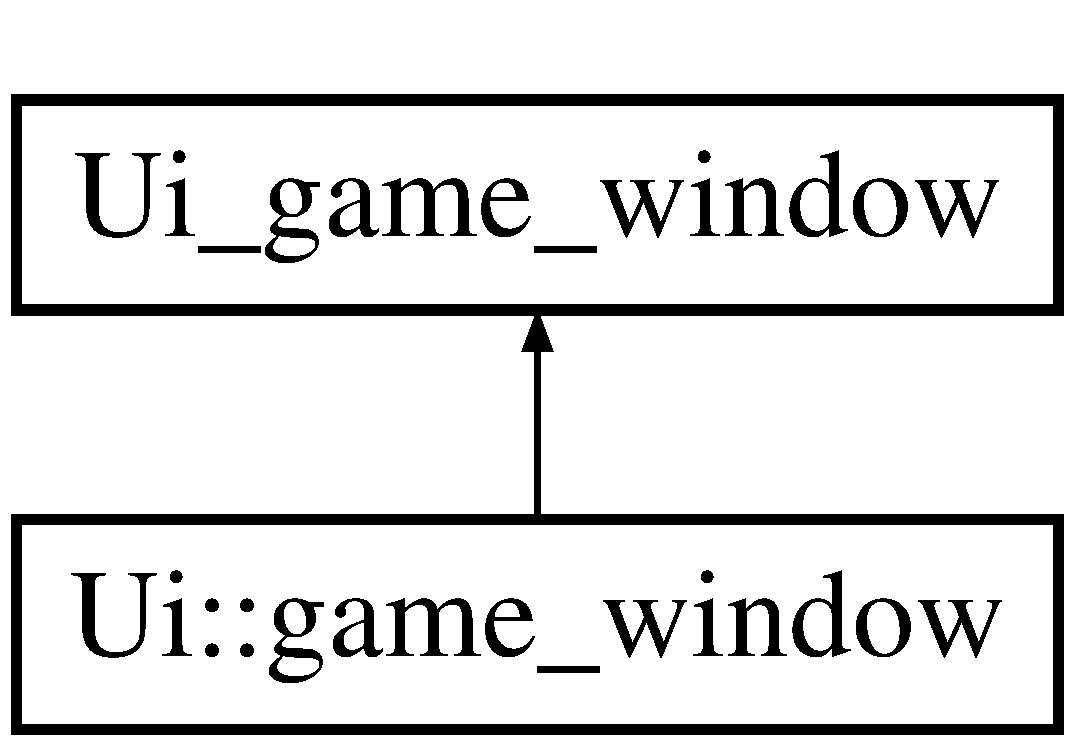
\includegraphics[height=2.000000cm]{classUi__game__window}
\end{center}
\end{figure}
\subsection*{Public Member Functions}
\begin{DoxyCompactItemize}
\item 
void \hyperlink{classUi__game__window_a3a7824fa0cac2ee95145c841c6615143}{setup\-Ui} (Q\-Main\-Window $\ast$\hyperlink{classgame__window}{game\-\_\-window})
\item 
void \hyperlink{classUi__game__window_af8b0343e4a4202b03c2a2038455c508a}{retranslate\-Ui} (Q\-Main\-Window $\ast$\hyperlink{classgame__window}{game\-\_\-window})
\end{DoxyCompactItemize}
\subsection*{Public Attributes}
\begin{DoxyCompactItemize}
\item 
Q\-Widget $\ast$ \hyperlink{classUi__game__window_aa46a61bfcdb8c9d7706974913e944cbe}{centralwidget}
\item 
Q\-Line\-Edit $\ast$ \hyperlink{classUi__game__window_a0881fadd6d3e567683404dd2aea66dd8}{command\-\_\-edit}
\item 
Q\-Label $\ast$ \hyperlink{classUi__game__window_a309b06ba0af4527d2e78f91d03bc08d4}{zadej\-\_\-prikaz\-\_\-label}
\item 
Q\-Label $\ast$ \hyperlink{classUi__game__window_a8b1b310fc381161f44c720fa8ea3c4d6}{when\-\_\-error\-\_\-label}
\item 
Q\-Push\-Button $\ast$ \hyperlink{classUi__game__window_aef389fef0c6667e488d979c2ba461237}{send\-\_\-command\-\_\-button}
\item 
Q\-Widget $\ast$ \hyperlink{classUi__game__window_a8447a074aadb12177aba7e7e1ba8cb61}{grid\-Layout\-Widget}
\item 
Q\-Grid\-Layout $\ast$ \hyperlink{classUi__game__window_af41420b2a865afe1600e82c56b788b86}{grid}
\item 
Q\-Menu\-Bar $\ast$ \hyperlink{classUi__game__window_a264dfe7db0e67d4a69d2d21ede691982}{menubar}
\end{DoxyCompactItemize}


\subsection{Member Function Documentation}
\hypertarget{classUi__game__window_af8b0343e4a4202b03c2a2038455c508a}{\index{Ui\-\_\-game\-\_\-window@{Ui\-\_\-game\-\_\-window}!retranslate\-Ui@{retranslate\-Ui}}
\index{retranslate\-Ui@{retranslate\-Ui}!Ui_game_window@{Ui\-\_\-game\-\_\-window}}
\subsubsection[{retranslate\-Ui}]{\setlength{\rightskip}{0pt plus 5cm}void Ui\-\_\-game\-\_\-window\-::retranslate\-Ui (
\begin{DoxyParamCaption}
\item[{Q\-Main\-Window $\ast$}]{game\-\_\-window}
\end{DoxyParamCaption}
)\hspace{0.3cm}{\ttfamily [inline]}}}\label{classUi__game__window_af8b0343e4a4202b03c2a2038455c508a}
\hypertarget{classUi__game__window_a3a7824fa0cac2ee95145c841c6615143}{\index{Ui\-\_\-game\-\_\-window@{Ui\-\_\-game\-\_\-window}!setup\-Ui@{setup\-Ui}}
\index{setup\-Ui@{setup\-Ui}!Ui_game_window@{Ui\-\_\-game\-\_\-window}}
\subsubsection[{setup\-Ui}]{\setlength{\rightskip}{0pt plus 5cm}void Ui\-\_\-game\-\_\-window\-::setup\-Ui (
\begin{DoxyParamCaption}
\item[{Q\-Main\-Window $\ast$}]{game\-\_\-window}
\end{DoxyParamCaption}
)\hspace{0.3cm}{\ttfamily [inline]}}}\label{classUi__game__window_a3a7824fa0cac2ee95145c841c6615143}


\subsection{Member Data Documentation}
\hypertarget{classUi__game__window_aa46a61bfcdb8c9d7706974913e944cbe}{\index{Ui\-\_\-game\-\_\-window@{Ui\-\_\-game\-\_\-window}!centralwidget@{centralwidget}}
\index{centralwidget@{centralwidget}!Ui_game_window@{Ui\-\_\-game\-\_\-window}}
\subsubsection[{centralwidget}]{\setlength{\rightskip}{0pt plus 5cm}Q\-Widget$\ast$ Ui\-\_\-game\-\_\-window\-::centralwidget}}\label{classUi__game__window_aa46a61bfcdb8c9d7706974913e944cbe}
\hypertarget{classUi__game__window_a0881fadd6d3e567683404dd2aea66dd8}{\index{Ui\-\_\-game\-\_\-window@{Ui\-\_\-game\-\_\-window}!command\-\_\-edit@{command\-\_\-edit}}
\index{command\-\_\-edit@{command\-\_\-edit}!Ui_game_window@{Ui\-\_\-game\-\_\-window}}
\subsubsection[{command\-\_\-edit}]{\setlength{\rightskip}{0pt plus 5cm}Q\-Line\-Edit$\ast$ Ui\-\_\-game\-\_\-window\-::command\-\_\-edit}}\label{classUi__game__window_a0881fadd6d3e567683404dd2aea66dd8}
\hypertarget{classUi__game__window_af41420b2a865afe1600e82c56b788b86}{\index{Ui\-\_\-game\-\_\-window@{Ui\-\_\-game\-\_\-window}!grid@{grid}}
\index{grid@{grid}!Ui_game_window@{Ui\-\_\-game\-\_\-window}}
\subsubsection[{grid}]{\setlength{\rightskip}{0pt plus 5cm}Q\-Grid\-Layout$\ast$ Ui\-\_\-game\-\_\-window\-::grid}}\label{classUi__game__window_af41420b2a865afe1600e82c56b788b86}
\hypertarget{classUi__game__window_a8447a074aadb12177aba7e7e1ba8cb61}{\index{Ui\-\_\-game\-\_\-window@{Ui\-\_\-game\-\_\-window}!grid\-Layout\-Widget@{grid\-Layout\-Widget}}
\index{grid\-Layout\-Widget@{grid\-Layout\-Widget}!Ui_game_window@{Ui\-\_\-game\-\_\-window}}
\subsubsection[{grid\-Layout\-Widget}]{\setlength{\rightskip}{0pt plus 5cm}Q\-Widget$\ast$ Ui\-\_\-game\-\_\-window\-::grid\-Layout\-Widget}}\label{classUi__game__window_a8447a074aadb12177aba7e7e1ba8cb61}
\hypertarget{classUi__game__window_a264dfe7db0e67d4a69d2d21ede691982}{\index{Ui\-\_\-game\-\_\-window@{Ui\-\_\-game\-\_\-window}!menubar@{menubar}}
\index{menubar@{menubar}!Ui_game_window@{Ui\-\_\-game\-\_\-window}}
\subsubsection[{menubar}]{\setlength{\rightskip}{0pt plus 5cm}Q\-Menu\-Bar$\ast$ Ui\-\_\-game\-\_\-window\-::menubar}}\label{classUi__game__window_a264dfe7db0e67d4a69d2d21ede691982}
\hypertarget{classUi__game__window_aef389fef0c6667e488d979c2ba461237}{\index{Ui\-\_\-game\-\_\-window@{Ui\-\_\-game\-\_\-window}!send\-\_\-command\-\_\-button@{send\-\_\-command\-\_\-button}}
\index{send\-\_\-command\-\_\-button@{send\-\_\-command\-\_\-button}!Ui_game_window@{Ui\-\_\-game\-\_\-window}}
\subsubsection[{send\-\_\-command\-\_\-button}]{\setlength{\rightskip}{0pt plus 5cm}Q\-Push\-Button$\ast$ Ui\-\_\-game\-\_\-window\-::send\-\_\-command\-\_\-button}}\label{classUi__game__window_aef389fef0c6667e488d979c2ba461237}
\hypertarget{classUi__game__window_a8b1b310fc381161f44c720fa8ea3c4d6}{\index{Ui\-\_\-game\-\_\-window@{Ui\-\_\-game\-\_\-window}!when\-\_\-error\-\_\-label@{when\-\_\-error\-\_\-label}}
\index{when\-\_\-error\-\_\-label@{when\-\_\-error\-\_\-label}!Ui_game_window@{Ui\-\_\-game\-\_\-window}}
\subsubsection[{when\-\_\-error\-\_\-label}]{\setlength{\rightskip}{0pt plus 5cm}Q\-Label$\ast$ Ui\-\_\-game\-\_\-window\-::when\-\_\-error\-\_\-label}}\label{classUi__game__window_a8b1b310fc381161f44c720fa8ea3c4d6}
\hypertarget{classUi__game__window_a309b06ba0af4527d2e78f91d03bc08d4}{\index{Ui\-\_\-game\-\_\-window@{Ui\-\_\-game\-\_\-window}!zadej\-\_\-prikaz\-\_\-label@{zadej\-\_\-prikaz\-\_\-label}}
\index{zadej\-\_\-prikaz\-\_\-label@{zadej\-\_\-prikaz\-\_\-label}!Ui_game_window@{Ui\-\_\-game\-\_\-window}}
\subsubsection[{zadej\-\_\-prikaz\-\_\-label}]{\setlength{\rightskip}{0pt plus 5cm}Q\-Label$\ast$ Ui\-\_\-game\-\_\-window\-::zadej\-\_\-prikaz\-\_\-label}}\label{classUi__game__window_a309b06ba0af4527d2e78f91d03bc08d4}


The documentation for this class was generated from the following file\-:\begin{DoxyCompactItemize}
\item 
gui/build-\/client\-\_\-bludiste-\/\-Desktop-\/\-Debug/\hyperlink{ui__game__window_8h}{ui\-\_\-game\-\_\-window.\-h}\end{DoxyCompactItemize}

\hypertarget{classUi__server__connection__window}{\section{Ui\-\_\-server\-\_\-connection\-\_\-window Class Reference}
\label{classUi__server__connection__window}\index{Ui\-\_\-server\-\_\-connection\-\_\-window@{Ui\-\_\-server\-\_\-connection\-\_\-window}}
}


{\ttfamily \#include $<$ui\-\_\-server\-\_\-connection\-\_\-window.\-h$>$}

Inheritance diagram for Ui\-\_\-server\-\_\-connection\-\_\-window\-:\begin{figure}[H]
\begin{center}
\leavevmode
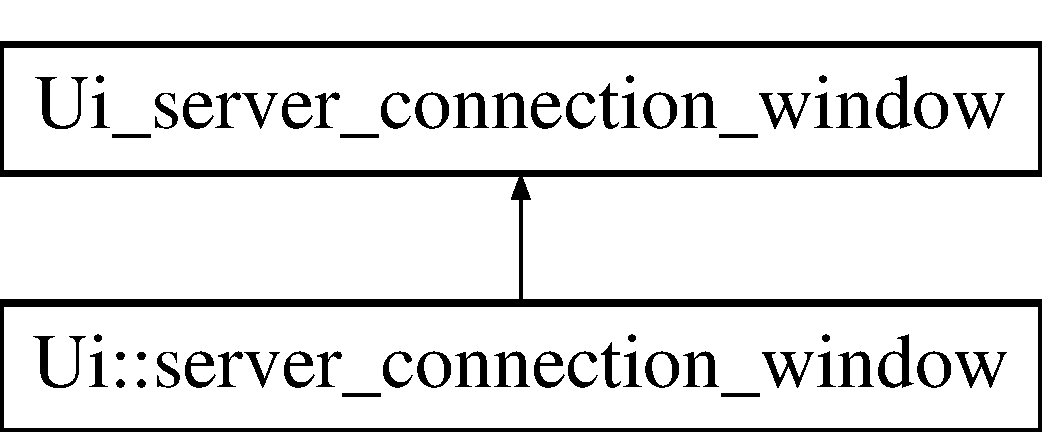
\includegraphics[height=2.000000cm]{classUi__server__connection__window}
\end{center}
\end{figure}
\subsection*{Public Member Functions}
\begin{DoxyCompactItemize}
\item 
void \hyperlink{classUi__server__connection__window_acbdbebbb76dc1504d0b63bdc3b7ad75a}{setup\-Ui} (Q\-Main\-Window $\ast$\hyperlink{classserver__connection__window}{server\-\_\-connection\-\_\-window})
\item 
void \hyperlink{classUi__server__connection__window_ab315b21ffbaaf416bbe1bc639798e666}{retranslate\-Ui} (Q\-Main\-Window $\ast$\hyperlink{classserver__connection__window}{server\-\_\-connection\-\_\-window})
\end{DoxyCompactItemize}
\subsection*{Public Attributes}
\begin{DoxyCompactItemize}
\item 
Q\-Widget $\ast$ \hyperlink{classUi__server__connection__window_a9b76c80b2439ac5363c319758e13fdba}{centralwidget}
\item 
Q\-Label $\ast$ \hyperlink{classUi__server__connection__window_a96edc08348d65093b103b9d0b1eaa024}{label}
\item 
Q\-Line\-Edit $\ast$ \hyperlink{classUi__server__connection__window_a2d2674c180c60ce36dc7b01988779448}{server\-\_\-name\-\_\-edit}
\item 
Q\-Push\-Button $\ast$ \hyperlink{classUi__server__connection__window_a42b1801ba78d2d54b731f74a566d112b}{server\-\_\-connect\-\_\-button}
\item 
Q\-Label $\ast$ \hyperlink{classUi__server__connection__window_aaa93b479324f97d626b83f2286c298a8}{when\-\_\-error\-\_\-label}
\item 
Q\-Menu\-Bar $\ast$ \hyperlink{classUi__server__connection__window_abe650faec1c385db9a7ec4efa7f0bd88}{menubar}
\end{DoxyCompactItemize}


\subsection{Member Function Documentation}
\hypertarget{classUi__server__connection__window_ab315b21ffbaaf416bbe1bc639798e666}{\index{Ui\-\_\-server\-\_\-connection\-\_\-window@{Ui\-\_\-server\-\_\-connection\-\_\-window}!retranslate\-Ui@{retranslate\-Ui}}
\index{retranslate\-Ui@{retranslate\-Ui}!Ui_server_connection_window@{Ui\-\_\-server\-\_\-connection\-\_\-window}}
\subsubsection[{retranslate\-Ui}]{\setlength{\rightskip}{0pt plus 5cm}void Ui\-\_\-server\-\_\-connection\-\_\-window\-::retranslate\-Ui (
\begin{DoxyParamCaption}
\item[{Q\-Main\-Window $\ast$}]{server\-\_\-connection\-\_\-window}
\end{DoxyParamCaption}
)\hspace{0.3cm}{\ttfamily [inline]}}}\label{classUi__server__connection__window_ab315b21ffbaaf416bbe1bc639798e666}
\hypertarget{classUi__server__connection__window_acbdbebbb76dc1504d0b63bdc3b7ad75a}{\index{Ui\-\_\-server\-\_\-connection\-\_\-window@{Ui\-\_\-server\-\_\-connection\-\_\-window}!setup\-Ui@{setup\-Ui}}
\index{setup\-Ui@{setup\-Ui}!Ui_server_connection_window@{Ui\-\_\-server\-\_\-connection\-\_\-window}}
\subsubsection[{setup\-Ui}]{\setlength{\rightskip}{0pt plus 5cm}void Ui\-\_\-server\-\_\-connection\-\_\-window\-::setup\-Ui (
\begin{DoxyParamCaption}
\item[{Q\-Main\-Window $\ast$}]{server\-\_\-connection\-\_\-window}
\end{DoxyParamCaption}
)\hspace{0.3cm}{\ttfamily [inline]}}}\label{classUi__server__connection__window_acbdbebbb76dc1504d0b63bdc3b7ad75a}


\subsection{Member Data Documentation}
\hypertarget{classUi__server__connection__window_a9b76c80b2439ac5363c319758e13fdba}{\index{Ui\-\_\-server\-\_\-connection\-\_\-window@{Ui\-\_\-server\-\_\-connection\-\_\-window}!centralwidget@{centralwidget}}
\index{centralwidget@{centralwidget}!Ui_server_connection_window@{Ui\-\_\-server\-\_\-connection\-\_\-window}}
\subsubsection[{centralwidget}]{\setlength{\rightskip}{0pt plus 5cm}Q\-Widget$\ast$ Ui\-\_\-server\-\_\-connection\-\_\-window\-::centralwidget}}\label{classUi__server__connection__window_a9b76c80b2439ac5363c319758e13fdba}
\hypertarget{classUi__server__connection__window_a96edc08348d65093b103b9d0b1eaa024}{\index{Ui\-\_\-server\-\_\-connection\-\_\-window@{Ui\-\_\-server\-\_\-connection\-\_\-window}!label@{label}}
\index{label@{label}!Ui_server_connection_window@{Ui\-\_\-server\-\_\-connection\-\_\-window}}
\subsubsection[{label}]{\setlength{\rightskip}{0pt plus 5cm}Q\-Label$\ast$ Ui\-\_\-server\-\_\-connection\-\_\-window\-::label}}\label{classUi__server__connection__window_a96edc08348d65093b103b9d0b1eaa024}
\hypertarget{classUi__server__connection__window_abe650faec1c385db9a7ec4efa7f0bd88}{\index{Ui\-\_\-server\-\_\-connection\-\_\-window@{Ui\-\_\-server\-\_\-connection\-\_\-window}!menubar@{menubar}}
\index{menubar@{menubar}!Ui_server_connection_window@{Ui\-\_\-server\-\_\-connection\-\_\-window}}
\subsubsection[{menubar}]{\setlength{\rightskip}{0pt plus 5cm}Q\-Menu\-Bar$\ast$ Ui\-\_\-server\-\_\-connection\-\_\-window\-::menubar}}\label{classUi__server__connection__window_abe650faec1c385db9a7ec4efa7f0bd88}
\hypertarget{classUi__server__connection__window_a42b1801ba78d2d54b731f74a566d112b}{\index{Ui\-\_\-server\-\_\-connection\-\_\-window@{Ui\-\_\-server\-\_\-connection\-\_\-window}!server\-\_\-connect\-\_\-button@{server\-\_\-connect\-\_\-button}}
\index{server\-\_\-connect\-\_\-button@{server\-\_\-connect\-\_\-button}!Ui_server_connection_window@{Ui\-\_\-server\-\_\-connection\-\_\-window}}
\subsubsection[{server\-\_\-connect\-\_\-button}]{\setlength{\rightskip}{0pt plus 5cm}Q\-Push\-Button$\ast$ Ui\-\_\-server\-\_\-connection\-\_\-window\-::server\-\_\-connect\-\_\-button}}\label{classUi__server__connection__window_a42b1801ba78d2d54b731f74a566d112b}
\hypertarget{classUi__server__connection__window_a2d2674c180c60ce36dc7b01988779448}{\index{Ui\-\_\-server\-\_\-connection\-\_\-window@{Ui\-\_\-server\-\_\-connection\-\_\-window}!server\-\_\-name\-\_\-edit@{server\-\_\-name\-\_\-edit}}
\index{server\-\_\-name\-\_\-edit@{server\-\_\-name\-\_\-edit}!Ui_server_connection_window@{Ui\-\_\-server\-\_\-connection\-\_\-window}}
\subsubsection[{server\-\_\-name\-\_\-edit}]{\setlength{\rightskip}{0pt plus 5cm}Q\-Line\-Edit$\ast$ Ui\-\_\-server\-\_\-connection\-\_\-window\-::server\-\_\-name\-\_\-edit}}\label{classUi__server__connection__window_a2d2674c180c60ce36dc7b01988779448}
\hypertarget{classUi__server__connection__window_aaa93b479324f97d626b83f2286c298a8}{\index{Ui\-\_\-server\-\_\-connection\-\_\-window@{Ui\-\_\-server\-\_\-connection\-\_\-window}!when\-\_\-error\-\_\-label@{when\-\_\-error\-\_\-label}}
\index{when\-\_\-error\-\_\-label@{when\-\_\-error\-\_\-label}!Ui_server_connection_window@{Ui\-\_\-server\-\_\-connection\-\_\-window}}
\subsubsection[{when\-\_\-error\-\_\-label}]{\setlength{\rightskip}{0pt plus 5cm}Q\-Label$\ast$ Ui\-\_\-server\-\_\-connection\-\_\-window\-::when\-\_\-error\-\_\-label}}\label{classUi__server__connection__window_aaa93b479324f97d626b83f2286c298a8}


The documentation for this class was generated from the following file\-:\begin{DoxyCompactItemize}
\item 
gui/build-\/client\-\_\-bludiste-\/\-Desktop-\/\-Debug/\hyperlink{ui__server__connection__window_8h}{ui\-\_\-server\-\_\-connection\-\_\-window.\-h}\end{DoxyCompactItemize}

\hypertarget{classUi__Setup__menu}{\section{Ui\-\_\-\-Setup\-\_\-menu Class Reference}
\label{classUi__Setup__menu}\index{Ui\-\_\-\-Setup\-\_\-menu@{Ui\-\_\-\-Setup\-\_\-menu}}
}


{\ttfamily \#include $<$ui\-\_\-setup\-\_\-menu.\-h$>$}

Inheritance diagram for Ui\-\_\-\-Setup\-\_\-menu\-:\begin{figure}[H]
\begin{center}
\leavevmode
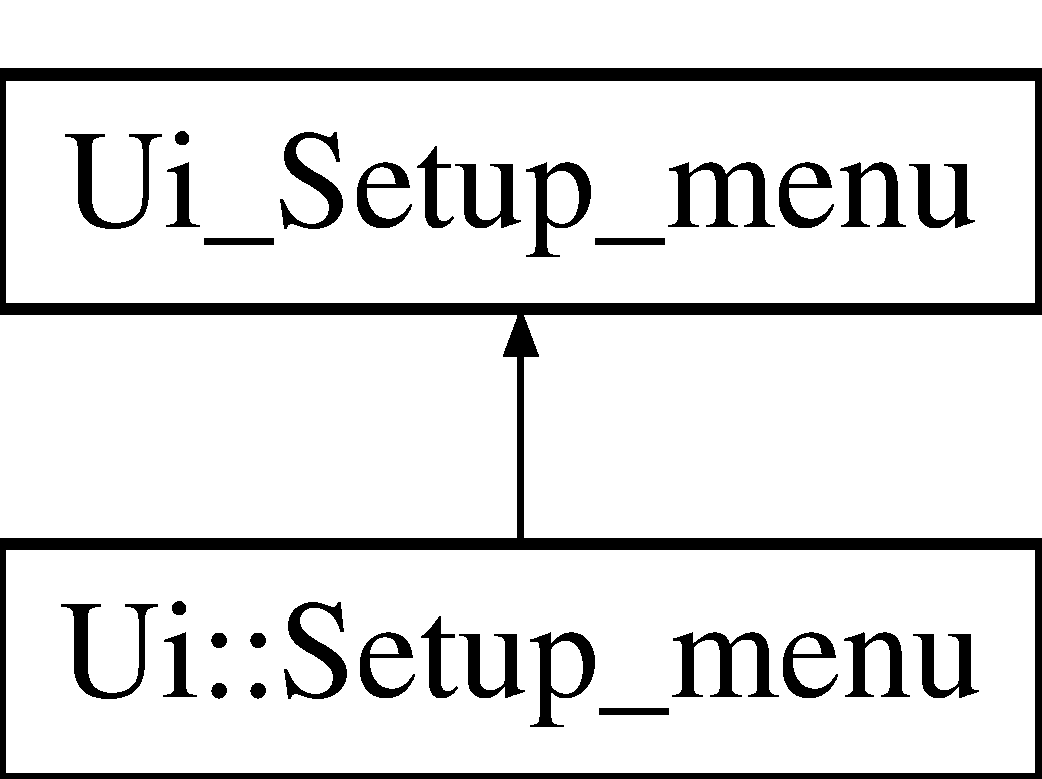
\includegraphics[height=2.000000cm]{classUi__Setup__menu}
\end{center}
\end{figure}
\subsection*{Public Member Functions}
\begin{DoxyCompactItemize}
\item 
void \hyperlink{classUi__Setup__menu_a955ec09b4541d88263c2a8be30a0d713}{setup\-Ui} (Q\-Main\-Window $\ast$Setup\-\_\-menu)
\item 
void \hyperlink{classUi__Setup__menu_a751af76f1c0f346abae17d3655bdde2b}{retranslate\-Ui} (Q\-Main\-Window $\ast$Setup\-\_\-menu)
\end{DoxyCompactItemize}
\subsection*{Public Attributes}
\begin{DoxyCompactItemize}
\item 
Q\-Widget $\ast$ \hyperlink{classUi__Setup__menu_a8ad7b9373da2ac90d9d7a70bacccb140}{central\-Widget}
\item 
Q\-Menu\-Bar $\ast$ \hyperlink{classUi__Setup__menu_a172549e1b5b0799af6b39eae5a58c6f7}{menu\-Bar}
\item 
Q\-Tool\-Bar $\ast$ \hyperlink{classUi__Setup__menu_a1b4525597f5e83a2eb1afd93ba044a06}{main\-Tool\-Bar}
\item 
Q\-Status\-Bar $\ast$ \hyperlink{classUi__Setup__menu_a4f657b28ad5893177d7f88f0675a0a4e}{status\-Bar}
\end{DoxyCompactItemize}


\subsection{Member Function Documentation}
\hypertarget{classUi__Setup__menu_a751af76f1c0f346abae17d3655bdde2b}{\index{Ui\-\_\-\-Setup\-\_\-menu@{Ui\-\_\-\-Setup\-\_\-menu}!retranslate\-Ui@{retranslate\-Ui}}
\index{retranslate\-Ui@{retranslate\-Ui}!Ui_Setup_menu@{Ui\-\_\-\-Setup\-\_\-menu}}
\subsubsection[{retranslate\-Ui}]{\setlength{\rightskip}{0pt plus 5cm}void Ui\-\_\-\-Setup\-\_\-menu\-::retranslate\-Ui (
\begin{DoxyParamCaption}
\item[{Q\-Main\-Window $\ast$}]{Setup\-\_\-menu}
\end{DoxyParamCaption}
)\hspace{0.3cm}{\ttfamily [inline]}}}\label{classUi__Setup__menu_a751af76f1c0f346abae17d3655bdde2b}
\hypertarget{classUi__Setup__menu_a955ec09b4541d88263c2a8be30a0d713}{\index{Ui\-\_\-\-Setup\-\_\-menu@{Ui\-\_\-\-Setup\-\_\-menu}!setup\-Ui@{setup\-Ui}}
\index{setup\-Ui@{setup\-Ui}!Ui_Setup_menu@{Ui\-\_\-\-Setup\-\_\-menu}}
\subsubsection[{setup\-Ui}]{\setlength{\rightskip}{0pt plus 5cm}void Ui\-\_\-\-Setup\-\_\-menu\-::setup\-Ui (
\begin{DoxyParamCaption}
\item[{Q\-Main\-Window $\ast$}]{Setup\-\_\-menu}
\end{DoxyParamCaption}
)\hspace{0.3cm}{\ttfamily [inline]}}}\label{classUi__Setup__menu_a955ec09b4541d88263c2a8be30a0d713}


\subsection{Member Data Documentation}
\hypertarget{classUi__Setup__menu_a8ad7b9373da2ac90d9d7a70bacccb140}{\index{Ui\-\_\-\-Setup\-\_\-menu@{Ui\-\_\-\-Setup\-\_\-menu}!central\-Widget@{central\-Widget}}
\index{central\-Widget@{central\-Widget}!Ui_Setup_menu@{Ui\-\_\-\-Setup\-\_\-menu}}
\subsubsection[{central\-Widget}]{\setlength{\rightskip}{0pt plus 5cm}Q\-Widget$\ast$ Ui\-\_\-\-Setup\-\_\-menu\-::central\-Widget}}\label{classUi__Setup__menu_a8ad7b9373da2ac90d9d7a70bacccb140}
\hypertarget{classUi__Setup__menu_a1b4525597f5e83a2eb1afd93ba044a06}{\index{Ui\-\_\-\-Setup\-\_\-menu@{Ui\-\_\-\-Setup\-\_\-menu}!main\-Tool\-Bar@{main\-Tool\-Bar}}
\index{main\-Tool\-Bar@{main\-Tool\-Bar}!Ui_Setup_menu@{Ui\-\_\-\-Setup\-\_\-menu}}
\subsubsection[{main\-Tool\-Bar}]{\setlength{\rightskip}{0pt plus 5cm}Q\-Tool\-Bar$\ast$ Ui\-\_\-\-Setup\-\_\-menu\-::main\-Tool\-Bar}}\label{classUi__Setup__menu_a1b4525597f5e83a2eb1afd93ba044a06}
\hypertarget{classUi__Setup__menu_a172549e1b5b0799af6b39eae5a58c6f7}{\index{Ui\-\_\-\-Setup\-\_\-menu@{Ui\-\_\-\-Setup\-\_\-menu}!menu\-Bar@{menu\-Bar}}
\index{menu\-Bar@{menu\-Bar}!Ui_Setup_menu@{Ui\-\_\-\-Setup\-\_\-menu}}
\subsubsection[{menu\-Bar}]{\setlength{\rightskip}{0pt plus 5cm}Q\-Menu\-Bar$\ast$ Ui\-\_\-\-Setup\-\_\-menu\-::menu\-Bar}}\label{classUi__Setup__menu_a172549e1b5b0799af6b39eae5a58c6f7}
\hypertarget{classUi__Setup__menu_a4f657b28ad5893177d7f88f0675a0a4e}{\index{Ui\-\_\-\-Setup\-\_\-menu@{Ui\-\_\-\-Setup\-\_\-menu}!status\-Bar@{status\-Bar}}
\index{status\-Bar@{status\-Bar}!Ui_Setup_menu@{Ui\-\_\-\-Setup\-\_\-menu}}
\subsubsection[{status\-Bar}]{\setlength{\rightskip}{0pt plus 5cm}Q\-Status\-Bar$\ast$ Ui\-\_\-\-Setup\-\_\-menu\-::status\-Bar}}\label{classUi__Setup__menu_a4f657b28ad5893177d7f88f0675a0a4e}


The documentation for this class was generated from the following file\-:\begin{DoxyCompactItemize}
\item 
\hyperlink{ui__setup__menu_8h}{ui\-\_\-setup\-\_\-menu.\-h}\end{DoxyCompactItemize}

\chapter{File Documentation}
\hypertarget{bludiste2014-cli_8cpp}{\section{bludiste2014-\/cli.cpp File Reference}
\label{bludiste2014-cli_8cpp}\index{bludiste2014-\/cli.\-cpp@{bludiste2014-\/cli.\-cpp}}
}
{\ttfamily \#include \char`\"{}client\-\_\-cli.\-h\char`\"{}}\\*
{\ttfamily \#include $<$Q\-Core\-Application$>$}\\*
{\ttfamily \#include $<$iostream$>$}\\*
{\ttfamily \#include \char`\"{}errors.\-h\char`\"{}}\\*
{\ttfamily \#include $<$stdio.\-h$>$}\\*
{\ttfamily \#include $<$locale.\-h$>$}\\*
\subsection*{Functions}
\begin{DoxyCompactItemize}
\item 
int \hyperlink{bludiste2014-cli_8cpp_a0ddf1224851353fc92bfbff6f499fa97}{main} (int argc, char $\ast$argv\mbox{[}$\,$\mbox{]})
\end{DoxyCompactItemize}


\subsection{Function Documentation}
\hypertarget{bludiste2014-cli_8cpp_a0ddf1224851353fc92bfbff6f499fa97}{\index{bludiste2014-\/cli.\-cpp@{bludiste2014-\/cli.\-cpp}!main@{main}}
\index{main@{main}!bludiste2014-cli.cpp@{bludiste2014-\/cli.\-cpp}}
\subsubsection[{main}]{\setlength{\rightskip}{0pt plus 5cm}int main (
\begin{DoxyParamCaption}
\item[{int}]{argc, }
\item[{char $\ast$}]{argv\mbox{[}$\,$\mbox{]}}
\end{DoxyParamCaption}
)}}\label{bludiste2014-cli_8cpp_a0ddf1224851353fc92bfbff6f499fa97}

\hypertarget{client_8cpp}{\section{client.\-cpp File Reference}
\label{client_8cpp}\index{client.\-cpp@{client.\-cpp}}
}
{\ttfamily \#include \char`\"{}client.\-h\char`\"{}}\\*
{\ttfamily \#include $<$iostream$>$}\\*
{\ttfamily \#include $<$Q\-Host\-Address$>$}\\*
{\ttfamily \#include \char`\"{}errors.\-h\char`\"{}}\\*
{\ttfamily \#include $<$string$>$}\\*
\subsection*{Functions}
\begin{DoxyCompactItemize}
\item 
void \hyperlink{client_8cpp_a4747cef8cf7e5a888ebd435ea07a6779}{read\-\_\-from\-\_\-socket} (Q\-Tcp\-Socket $\ast$client\-\_\-socket, std\-::string \&msg)
\end{DoxyCompactItemize}


\subsection{Detailed Description}
Soubor obsahující implementaci metod třídy \hyperlink{classClient}{Client} \begin{DoxyAuthor}{Author}
Michal Veselý (xvesel63) 
\end{DoxyAuthor}


\subsection{Function Documentation}
\hypertarget{client_8cpp_a4747cef8cf7e5a888ebd435ea07a6779}{\index{client.\-cpp@{client.\-cpp}!read\-\_\-from\-\_\-socket@{read\-\_\-from\-\_\-socket}}
\index{read\-\_\-from\-\_\-socket@{read\-\_\-from\-\_\-socket}!client.cpp@{client.\-cpp}}
\subsubsection[{read\-\_\-from\-\_\-socket}]{\setlength{\rightskip}{0pt plus 5cm}void read\-\_\-from\-\_\-socket (
\begin{DoxyParamCaption}
\item[{Q\-Tcp\-Socket $\ast$}]{client\-\_\-socket, }
\item[{std\-::string \&}]{msg}
\end{DoxyParamCaption}
)}}\label{client_8cpp_a4747cef8cf7e5a888ebd435ea07a6779}

\hypertarget{client_8h}{\section{client.\-h File Reference}
\label{client_8h}\index{client.\-h@{client.\-h}}
}
{\ttfamily \#include $<$iostream$>$}\\*
{\ttfamily \#include $<$Qt\-Core$>$}\\*
{\ttfamily \#include $<$Qt\-Network$>$}\\*
{\ttfamily \#include $<$string$>$}\\*
{\ttfamily \#include $<$Q\-Object$>$}\\*
{\ttfamily \#include $<$Q\-Tcp\-Socket$>$}\\*
\subsection*{Classes}
\begin{DoxyCompactItemize}
\item 
class \hyperlink{classClient}{Client}
\end{DoxyCompactItemize}


\subsection{Detailed Description}
Hlavičkový soubor pro třídu \hyperlink{classClient}{Client} \par
 Obsahuje aktualni stav hry\par
 Šířku a výšku hracího pole\par
 Barvu daného klienta\par
 Časovou prodlevu mezi tahy\par
 Pozici hráče ve hře \par
 počet navštívených polí a počet kroků\par
 čas strávený ve hře \par
 \begin{DoxyAuthor}{Author}
Michal Veselý (xvesel63) 
\end{DoxyAuthor}

\hypertarget{client__cli_8cpp}{\section{client\-\_\-cli.\-cpp File Reference}
\label{client__cli_8cpp}\index{client\-\_\-cli.\-cpp@{client\-\_\-cli.\-cpp}}
}
{\ttfamily \#include \char`\"{}client\-\_\-cli.\-h\char`\"{}}\\*


\subsection{Detailed Description}
Soubor obsahující implementaci metod třídy \hyperlink{classClient__cli}{Client\-\_\-cli}\par
 Rozšiřuje metody třídy Klient pouze o některé funkce výpisu, původní funkcionalita je jinak zachována a neměněna \begin{DoxyAuthor}{Author}
Michal Veselý (xvesel63) 
\end{DoxyAuthor}

\hypertarget{client__cli_8h}{\section{client\-\_\-cli.\-h File Reference}
\label{client__cli_8h}\index{client\-\_\-cli.\-h@{client\-\_\-cli.\-h}}
}
{\ttfamily \#include \char`\"{}client.\-h\char`\"{}}\\*
\subsection*{Classes}
\begin{DoxyCompactItemize}
\item 
class \hyperlink{classClient__cli}{Client\-\_\-cli}
\end{DoxyCompactItemize}


\subsection{Detailed Description}
Soubor obsahující implementaci hlavičky třídy \hyperlink{classClient__cli}{Client\-\_\-cli}\par
 Potomek Třídy \hyperlink{classClient}{Client}, jenž reimplementuje některé funkce tak, aby pracovali pouze s konzolí \begin{DoxyAuthor}{Author}
Michal Veselý (xvesel63) 
\end{DoxyAuthor}

\hypertarget{errors_8cpp}{\section{errors.\-cpp File Reference}
\label{errors_8cpp}\index{errors.\-cpp@{errors.\-cpp}}
}
{\ttfamily \#include \char`\"{}errors.\-h\char`\"{}}\\*


\subsection{Detailed Description}
Soubor obsahující implementaci metod třídy \hyperlink{classErrors}{Errors} \begin{DoxyAuthor}{Author}
Michal Veselý (xvesel63) 
\end{DoxyAuthor}

\hypertarget{errors_8h}{\section{errors.\-h File Reference}
\label{errors_8h}\index{errors.\-h@{errors.\-h}}
}
{\ttfamily \#include $<$iostream$>$}\\*
{\ttfamily \#include $<$string$>$}\\*
\subsection*{Classes}
\begin{DoxyCompactItemize}
\item 
class \hyperlink{classErrors}{Errors}
\end{DoxyCompactItemize}


\subsection{Detailed Description}
Obsahuje implementaci hlavičky třídy \hyperlink{classErrors}{Errors} \begin{DoxyAuthor}{Author}
Michal Veselý (xvesel63) 
\end{DoxyAuthor}

\hypertarget{moc__game__setup_8cpp}{\section{gui/build-\/client\-\_\-bludiste-\/\-Desktop-\/\-Debug/moc\-\_\-game\-\_\-setup.cpp File Reference}
\label{moc__game__setup_8cpp}\index{gui/build-\/client\-\_\-bludiste-\/\-Desktop-\/\-Debug/moc\-\_\-game\-\_\-setup.\-cpp@{gui/build-\/client\-\_\-bludiste-\/\-Desktop-\/\-Debug/moc\-\_\-game\-\_\-setup.\-cpp}}
}
{\ttfamily \#include \char`\"{}../client\-\_\-bludiste/game\-\_\-setup.\-h\char`\"{}}\\*
{\ttfamily \#include $<$Qt\-Core/qbytearray.\-h$>$}\\*
{\ttfamily \#include $<$Qt\-Core/qmetatype.\-h$>$}\\*
\subsection*{Classes}
\begin{DoxyCompactItemize}
\item 
struct \hyperlink{structqt__meta__stringdata__game__setup__t}{qt\-\_\-meta\-\_\-stringdata\-\_\-game\-\_\-setup\-\_\-t}
\end{DoxyCompactItemize}
\subsection*{Macros}
\begin{DoxyCompactItemize}
\item 
\#define \hyperlink{moc__game__setup_8cpp_a75bb9482d242cde0a06c9dbdc6b83abe}{Q\-T\-\_\-\-M\-O\-C\-\_\-\-L\-I\-T\-E\-R\-A\-L}(idx, ofs, len)
\end{DoxyCompactItemize}


\subsection{Macro Definition Documentation}
\hypertarget{moc__game__setup_8cpp_a75bb9482d242cde0a06c9dbdc6b83abe}{\index{moc\-\_\-game\-\_\-setup.\-cpp@{moc\-\_\-game\-\_\-setup.\-cpp}!Q\-T\-\_\-\-M\-O\-C\-\_\-\-L\-I\-T\-E\-R\-A\-L@{Q\-T\-\_\-\-M\-O\-C\-\_\-\-L\-I\-T\-E\-R\-A\-L}}
\index{Q\-T\-\_\-\-M\-O\-C\-\_\-\-L\-I\-T\-E\-R\-A\-L@{Q\-T\-\_\-\-M\-O\-C\-\_\-\-L\-I\-T\-E\-R\-A\-L}!moc_game_setup.cpp@{moc\-\_\-game\-\_\-setup.\-cpp}}
\subsubsection[{Q\-T\-\_\-\-M\-O\-C\-\_\-\-L\-I\-T\-E\-R\-A\-L}]{\setlength{\rightskip}{0pt plus 5cm}\#define Q\-T\-\_\-\-M\-O\-C\-\_\-\-L\-I\-T\-E\-R\-A\-L(
\begin{DoxyParamCaption}
\item[{}]{idx, }
\item[{}]{ofs, }
\item[{}]{len}
\end{DoxyParamCaption}
)}}\label{moc__game__setup_8cpp_a75bb9482d242cde0a06c9dbdc6b83abe}
{\bfseries Value\-:}
\begin{DoxyCode}
Q\_STATIC\_BYTE\_ARRAY\_DATA\_HEADER\_INITIALIZER\_WITH\_OFFSET(len, \(\backslash\)
    offsetof(\hyperlink{structqt__meta__stringdata__game__setup__t}{qt\_meta\_stringdata\_game\_setup\_t}, stringdata) + ofs \(\backslash\)
        - idx * \textcolor{keyword}{sizeof}(QByteArrayData) \(\backslash\)
    )
\end{DoxyCode}

\hypertarget{moc__game__window_8cpp}{\section{gui/build-\/client\-\_\-bludiste-\/\-Desktop-\/\-Debug/moc\-\_\-game\-\_\-window.cpp File Reference}
\label{moc__game__window_8cpp}\index{gui/build-\/client\-\_\-bludiste-\/\-Desktop-\/\-Debug/moc\-\_\-game\-\_\-window.\-cpp@{gui/build-\/client\-\_\-bludiste-\/\-Desktop-\/\-Debug/moc\-\_\-game\-\_\-window.\-cpp}}
}
{\ttfamily \#include \char`\"{}../client\-\_\-bludiste/game\-\_\-window.\-h\char`\"{}}\\*
{\ttfamily \#include $<$Qt\-Core/qbytearray.\-h$>$}\\*
{\ttfamily \#include $<$Qt\-Core/qmetatype.\-h$>$}\\*
\subsection*{Classes}
\begin{DoxyCompactItemize}
\item 
struct \hyperlink{structqt__meta__stringdata__game__window__t}{qt\-\_\-meta\-\_\-stringdata\-\_\-game\-\_\-window\-\_\-t}
\end{DoxyCompactItemize}
\subsection*{Macros}
\begin{DoxyCompactItemize}
\item 
\#define \hyperlink{moc__game__window_8cpp_a75bb9482d242cde0a06c9dbdc6b83abe}{Q\-T\-\_\-\-M\-O\-C\-\_\-\-L\-I\-T\-E\-R\-A\-L}(idx, ofs, len)
\end{DoxyCompactItemize}


\subsection{Macro Definition Documentation}
\hypertarget{moc__game__window_8cpp_a75bb9482d242cde0a06c9dbdc6b83abe}{\index{moc\-\_\-game\-\_\-window.\-cpp@{moc\-\_\-game\-\_\-window.\-cpp}!Q\-T\-\_\-\-M\-O\-C\-\_\-\-L\-I\-T\-E\-R\-A\-L@{Q\-T\-\_\-\-M\-O\-C\-\_\-\-L\-I\-T\-E\-R\-A\-L}}
\index{Q\-T\-\_\-\-M\-O\-C\-\_\-\-L\-I\-T\-E\-R\-A\-L@{Q\-T\-\_\-\-M\-O\-C\-\_\-\-L\-I\-T\-E\-R\-A\-L}!moc_game_window.cpp@{moc\-\_\-game\-\_\-window.\-cpp}}
\subsubsection[{Q\-T\-\_\-\-M\-O\-C\-\_\-\-L\-I\-T\-E\-R\-A\-L}]{\setlength{\rightskip}{0pt plus 5cm}\#define Q\-T\-\_\-\-M\-O\-C\-\_\-\-L\-I\-T\-E\-R\-A\-L(
\begin{DoxyParamCaption}
\item[{}]{idx, }
\item[{}]{ofs, }
\item[{}]{len}
\end{DoxyParamCaption}
)}}\label{moc__game__window_8cpp_a75bb9482d242cde0a06c9dbdc6b83abe}
{\bfseries Value\-:}
\begin{DoxyCode}
Q\_STATIC\_BYTE\_ARRAY\_DATA\_HEADER\_INITIALIZER\_WITH\_OFFSET(len, \(\backslash\)
    offsetof(\hyperlink{structqt__meta__stringdata__game__window__t}{qt\_meta\_stringdata\_game\_window\_t}, stringdata) + ofs \(\backslash\)
        - idx * \textcolor{keyword}{sizeof}(QByteArrayData) \(\backslash\)
    )
\end{DoxyCode}

\input{moc__server__connection__window_8cpp}
\input{ui__game__setup_8h}
\input{ui__game__window_8h}
\input{ui__server__connection__window_8h}
\hypertarget{bludiste2014_8cpp}{\section{gui/client\-\_\-bludiste/bludiste2014.cpp File Reference}
\label{bludiste2014_8cpp}\index{gui/client\-\_\-bludiste/bludiste2014.\-cpp@{gui/client\-\_\-bludiste/bludiste2014.\-cpp}}
}
{\ttfamily \#include \char`\"{}game\-\_\-setup.\-h\char`\"{}}\\*
{\ttfamily \#include \char`\"{}server\-\_\-connection\-\_\-window.\-h\char`\"{}}\\*
{\ttfamily \#include \char`\"{}game\-\_\-window.\-h\char`\"{}}\\*
{\ttfamily \#include $<$Q\-Application$>$}\\*
\subsection*{Functions}
\begin{DoxyCompactItemize}
\item 
int \hyperlink{bludiste2014_8cpp_a0ddf1224851353fc92bfbff6f499fa97}{main} (int argc, char $\ast$argv\mbox{[}$\,$\mbox{]})
\end{DoxyCompactItemize}


\subsection{Function Documentation}
\hypertarget{bludiste2014_8cpp_a0ddf1224851353fc92bfbff6f499fa97}{\index{bludiste2014.\-cpp@{bludiste2014.\-cpp}!main@{main}}
\index{main@{main}!bludiste2014.cpp@{bludiste2014.\-cpp}}
\subsubsection[{main}]{\setlength{\rightskip}{0pt plus 5cm}int main (
\begin{DoxyParamCaption}
\item[{int}]{argc, }
\item[{char $\ast$}]{argv\mbox{[}$\,$\mbox{]}}
\end{DoxyParamCaption}
)}}\label{bludiste2014_8cpp_a0ddf1224851353fc92bfbff6f499fa97}

\hypertarget{game__field_8cpp}{\section{gui/client\-\_\-bludiste/game\-\_\-field.cpp File Reference}
\label{game__field_8cpp}\index{gui/client\-\_\-bludiste/game\-\_\-field.\-cpp@{gui/client\-\_\-bludiste/game\-\_\-field.\-cpp}}
}
{\ttfamily \#include \char`\"{}game\-\_\-field.\-h\char`\"{}}\\*

\hypertarget{game__field_8h}{\section{gui/client\-\_\-bludiste/game\-\_\-field.h File Reference}
\label{game__field_8h}\index{gui/client\-\_\-bludiste/game\-\_\-field.\-h@{gui/client\-\_\-bludiste/game\-\_\-field.\-h}}
}
{\ttfamily \#include $<$Q\-Grid\-Layout$>$}\\*
{\ttfamily \#include $<$Q\-Label$>$}\\*
\subsection*{Classes}
\begin{DoxyCompactItemize}
\item 
class \hyperlink{classGame__field}{Game\-\_\-field}
\end{DoxyCompactItemize}


\subsection{Detailed Description}
Třída dědící od Q\-Grid\-Layout.\par
 Obsahuje všechny herní komponenty v podobě Q\-Pixmap a pole Q\-Labelů do kterých se tyto obrázky komponent zobrazují \begin{DoxyAuthor}{Author}
Michal Veselý (xvesel63) 
\end{DoxyAuthor}

\hypertarget{game__setup_8cpp}{\section{gui/client\-\_\-bludiste/game\-\_\-setup.cpp File Reference}
\label{game__setup_8cpp}\index{gui/client\-\_\-bludiste/game\-\_\-setup.\-cpp@{gui/client\-\_\-bludiste/game\-\_\-setup.\-cpp}}
}
{\ttfamily \#include \char`\"{}game\-\_\-setup.\-h\char`\"{}}\\*
{\ttfamily \#include \char`\"{}ui\-\_\-game\-\_\-setup.\-h\char`\"{}}\\*


\subsection{Detailed Description}
Implementuje metody třídy \hyperlink{classgame__setup}{game\-\_\-setup}. Vygenerované pomocí Q\-T Creator a přidáním implementace metod. \par
 Umožňuje připojení se do existující hry a vytvoření nové hry. Po vytvoření či připojení vytváří instanci třídy \hyperlink{classgame__window}{game\-\_\-window} pro samotné hraní hry. \begin{DoxyAuthor}{Author}
Michal Veselý (xvesel63) 
\end{DoxyAuthor}

\hypertarget{game__setup_8h}{\section{gui/client\-\_\-bludiste/game\-\_\-setup.h File Reference}
\label{game__setup_8h}\index{gui/client\-\_\-bludiste/game\-\_\-setup.\-h@{gui/client\-\_\-bludiste/game\-\_\-setup.\-h}}
}
{\ttfamily \#include $<$Q\-Main\-Window$>$}\\*
{\ttfamily \#include \char`\"{}./../../client.\-h\char`\"{}}\\*
{\ttfamily \#include $<$deque$>$}\\*
{\ttfamily \#include $<$Q\-List\-Widget$>$}\\*
{\ttfamily \#include \char`\"{}./../../errors.\-h\char`\"{}}\\*
{\ttfamily \#include \char`\"{}game\-\_\-window.\-h\char`\"{}}\\*
\subsection*{Classes}
\begin{DoxyCompactItemize}
\item 
class \hyperlink{classgame__setup}{game\-\_\-setup}
\end{DoxyCompactItemize}
\subsection*{Namespaces}
\begin{DoxyCompactItemize}
\item 
\hyperlink{namespaceUi}{Ui}
\end{DoxyCompactItemize}
\subsection*{Constant Groups}
\begin{DoxyCompactItemize}
\item 
\hyperlink{namespaceUi}{Ui}
\end{DoxyCompactItemize}


\subsection{Detailed Description}
Hlavičkový soubor pro definici třídy \hyperlink{classgame__setup}{game\-\_\-setup}. Vygenerován pomocí Q\-T Creator a přidáním některých atributů a metod. \par
 Vytváří se okno pro možnost připojení se k již existující hře nebo vytvoření nové hry. \begin{DoxyAuthor}{Author}
Michal Veselý (xvesel63) 
\end{DoxyAuthor}

\hypertarget{game__window_8cpp}{\section{gui/client\-\_\-bludiste/game\-\_\-window.cpp File Reference}
\label{game__window_8cpp}\index{gui/client\-\_\-bludiste/game\-\_\-window.\-cpp@{gui/client\-\_\-bludiste/game\-\_\-window.\-cpp}}
}
{\ttfamily \#include \char`\"{}game\-\_\-window.\-h\char`\"{}}\\*
{\ttfamily \#include \char`\"{}ui\-\_\-game\-\_\-window.\-h\char`\"{}}\\*
{\ttfamily \#include \char`\"{}./../../errors.\-h\char`\"{}}\\*


\subsection{Detailed Description}
Soubor implementující třídu \hyperlink{classgame__window}{game\-\_\-window}. Vygenerováno pomocí Q\-T Creator s rozšířením o některé atributy a metody.\par
 Implementuje hrací okno hry. Používá třídu \hyperlink{classGame__field}{Game\-\_\-field} pro zobrazení hrací plochy. \begin{DoxyAuthor}{Author}
Michal Veselý (xvesel63) 
\end{DoxyAuthor}

\hypertarget{game__window_8h}{\section{gui/client\-\_\-bludiste/game\-\_\-window.h File Reference}
\label{game__window_8h}\index{gui/client\-\_\-bludiste/game\-\_\-window.\-h@{gui/client\-\_\-bludiste/game\-\_\-window.\-h}}
}
{\ttfamily \#include $<$Q\-Main\-Window$>$}\\*
{\ttfamily \#include \char`\"{}./../../client.\-h\char`\"{}}\\*
{\ttfamily \#include \char`\"{}game\-\_\-window.\-h\char`\"{}}\\*
{\ttfamily \#include \char`\"{}game\-\_\-field.\-h\char`\"{}}\\*
\subsection*{Classes}
\begin{DoxyCompactItemize}
\item 
class \hyperlink{classgame__window}{game\-\_\-window}
\end{DoxyCompactItemize}
\subsection*{Namespaces}
\begin{DoxyCompactItemize}
\item 
\hyperlink{namespaceUi}{Ui}
\end{DoxyCompactItemize}
\subsection*{Constant Groups}
\begin{DoxyCompactItemize}
\item 
\hyperlink{namespaceUi}{Ui}
\end{DoxyCompactItemize}


\subsection{Detailed Description}
Hlavičkový soubor definující třídu \hyperlink{classgame__window}{game\-\_\-window}. Vygenerováno pomocí Q\-T Creator s rozšířením o některé atributy a metody.\par
 Je implementací okna ve kterém dochází k hraní hry. Importuje si třídu \hyperlink{classGame__field}{Game\-\_\-field}, která obsahuje matici hracího pole. \begin{DoxyAuthor}{Author}
Michal Veselý (xvesel63) 
\end{DoxyAuthor}

\input{server__connection__window_8cpp}
\input{server__connection__window_8h}
\input{ui__setup__menu_8h}
%--- End generated contents ---

% Index
\newpage
\phantomsection
\addcontentsline{toc}{part}{Index}
\printindex

\end{document}
